\documentclass{report}
\usepackage[utf8]{inputenc}
\usepackage{hyperref}
\usepackage{datetime}
\usepackage{graphicx}
\usepackage{subcaption}
\usepackage{float}
\usepackage{enumerate}

\graphicspath{./}

\title{Aquarium Care Guide}
\author{Gaultier Delbarre}
\date{\today}

\begin{document}

\maketitle

\tableofcontents

\newpage
\chapter{Introduction}
Howdy! Thank you for taking care of my aquariums! I have written this here guide to help you in taking care of the aquariums 
while I am away. Please read the entire guide before beginning maintenance on either of the aquariums, as there are some 
specific things to do for each one. This guide additionally contains information on how to set-up the RO/DI filter and 
produce RO/DI water. 

If you have any questions, or notice any errors on this guide, please tell me so that I may update it and send you the newest 
copy. The date at the top of the document indicates the last day I reviewed this guide. 

Especially for the saltwater aquarium, please follow all instructions in this guide carefully. Now, without further ado, 
here's the fun part!

\begin{figure}[h]
    \centering
    \begin{subfigure}{0.5\textwidth}
        \centering
        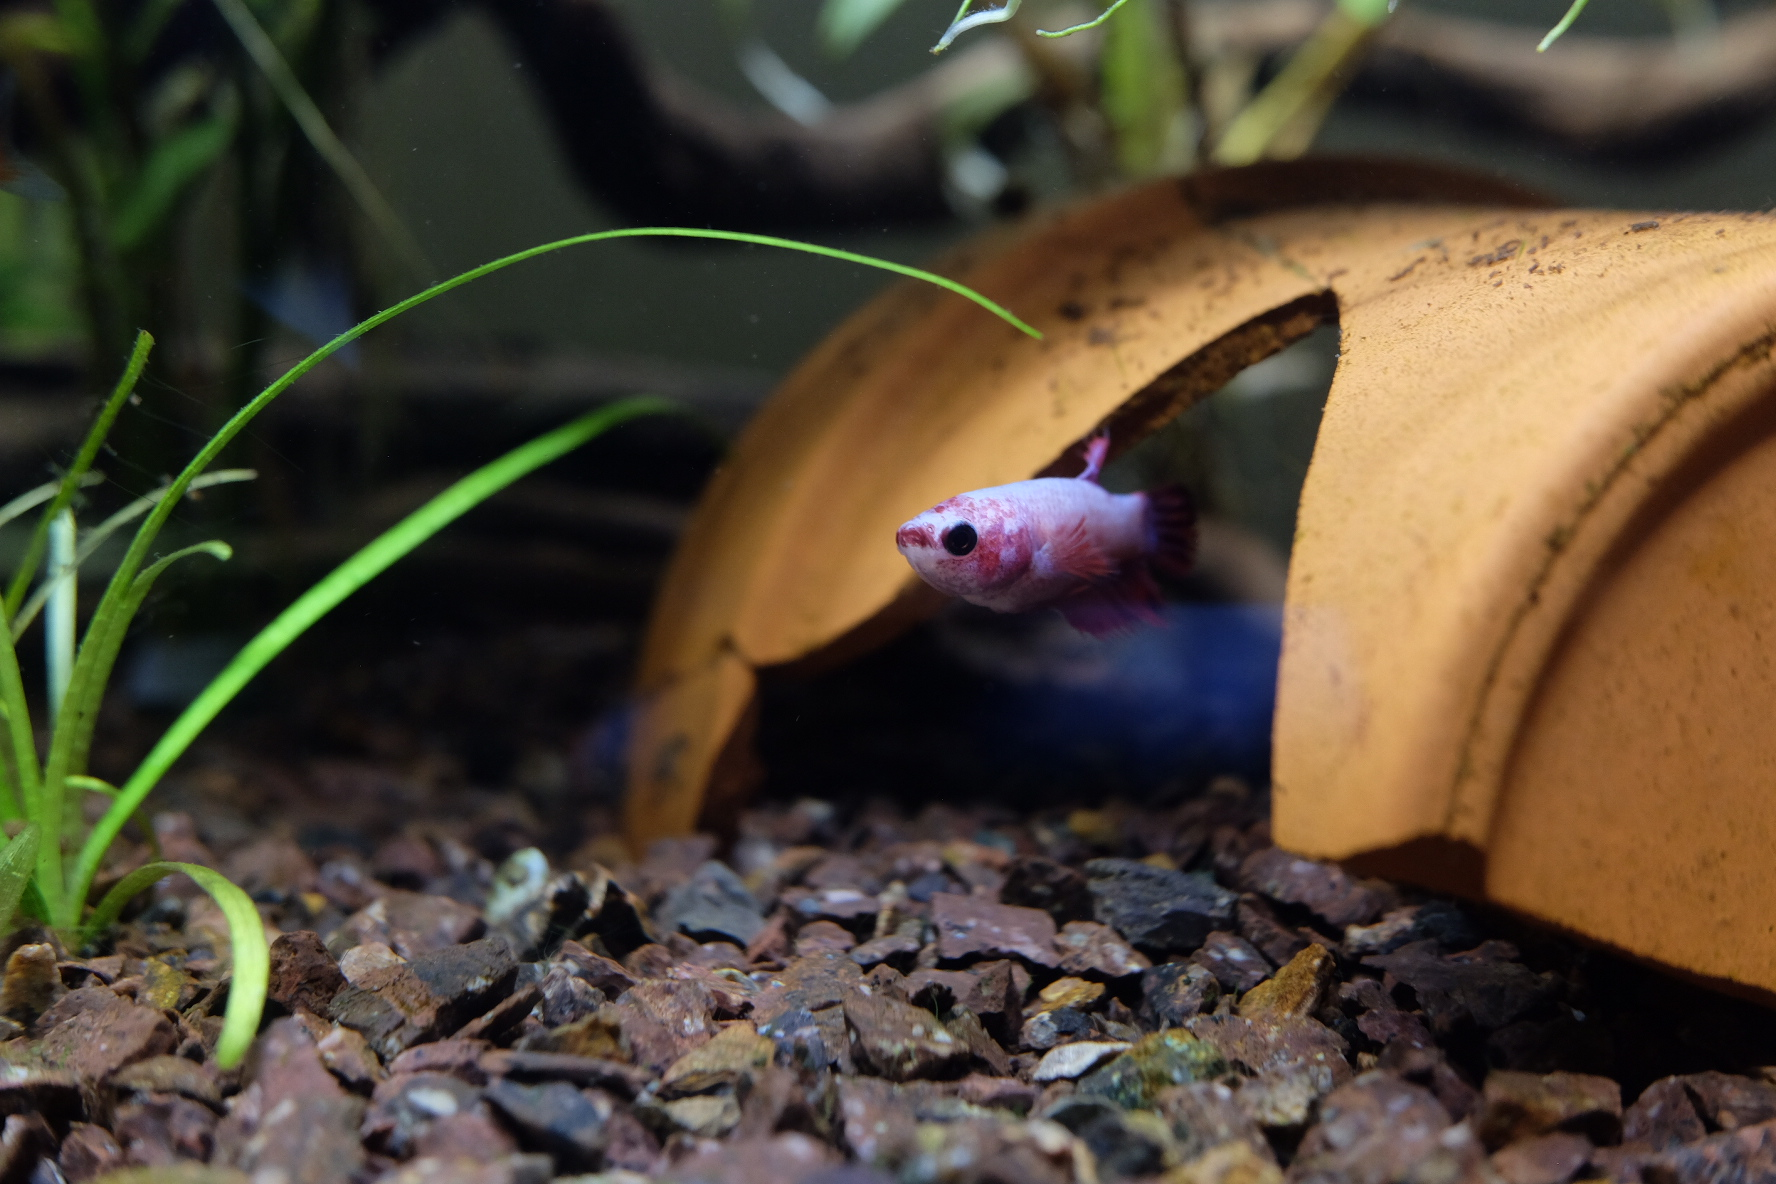
\includegraphics[width=0.9\textwidth]{betta1.jpg}
        \caption{Gertie}
    \end{subfigure}%
    \begin{subfigure}{0.5\textwidth}
        \centering
        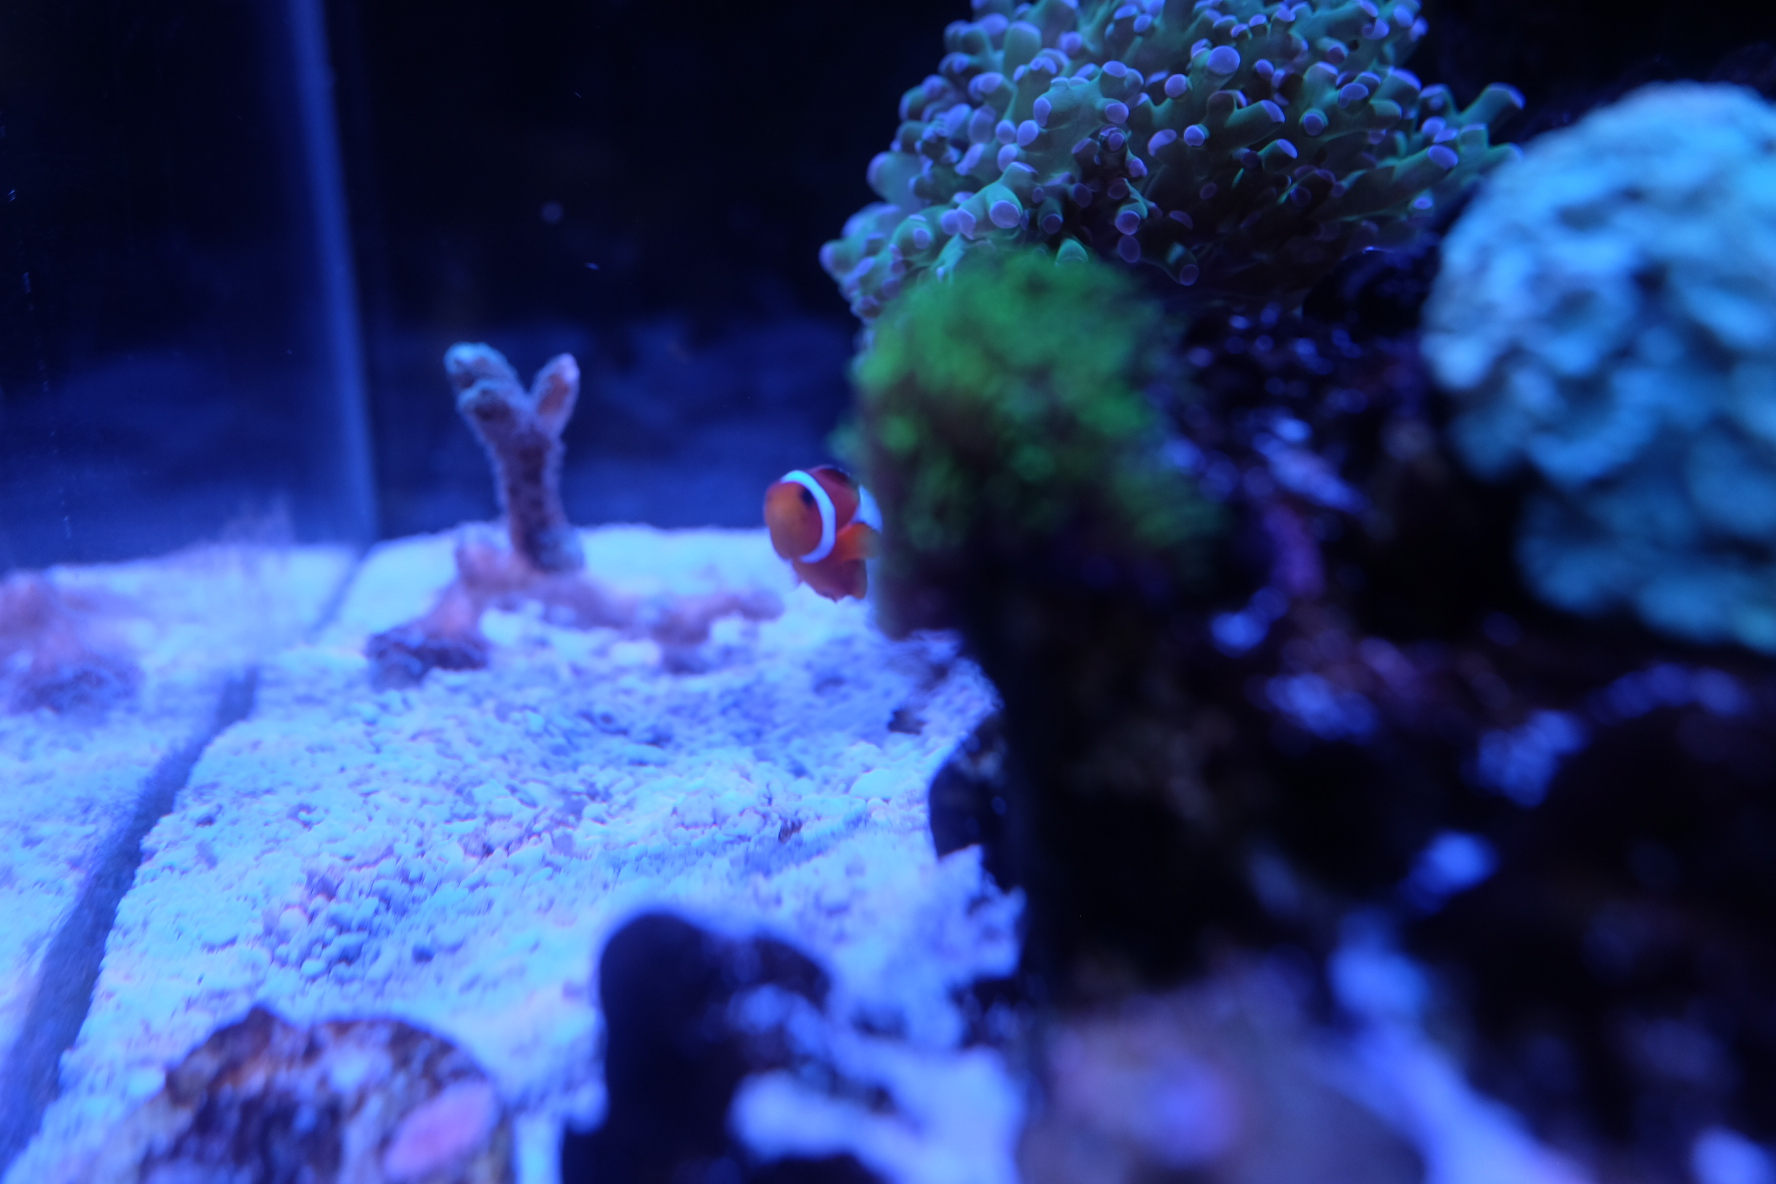
\includegraphics[width=0.9\textwidth]{cheddarpeek1.jpg}
        \caption{Cheddar}
    \end{subfigure}
    \caption{The Two Divas}
\end{figure}

\newpage
\chapter{RO/DI Water}
\label{sec:rodi}
\section{Introduction}
Both tanks exclusively use reverse osmosis deionized (RODI) water for their water changes and their top-up water. 

To make RO/DI water, you'll need to bring the RODI filter outside to the front porch of our house. The RODI filter is in an
Athleta bag near the aquariums and has a mess of tubes sticking out of it. Additionally, bring the 5-gallon jug labelled
"RODI ONLY" to fill it up. Please never put anything but RODI water in the "RODI ONLY" jug. 


\begin{figure}[H]
    \centering
    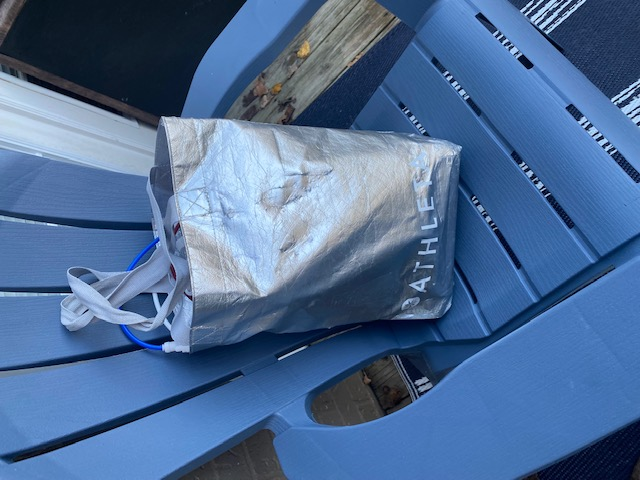
\includegraphics[width=0.65\textwidth, angle=-90]{RodiBag.jpg}
    \caption{The Athleta Bag}
\end{figure}

Remove the filter from the bag, being careful to only lift it by the hard white plastic portions, and not the tubes. 
Set the RODI filter on the cat house (the brown wooden box near the entrance to the porch). There are 3 different tubes that
go into or come out of the RODI filter. They are distinguishable by their color. The white tube has an adapter for a garden
water spout and is the input to the RODI filter. The red tube is the wastewater tube. RODI filters produce a lot of
wastewater, so you'll want to wedge the red tube between the slats in the porch floor to prevent the tube from spraying you 
with the water. Notice that there is a valve on the red tube. This valve helps increase the pressure across the RO membranes.
Lastly, the blue tube is the clean RODI water. You'll want to drop this into whatever container you're filling up.

\begin{figure}[H]
    \centering
    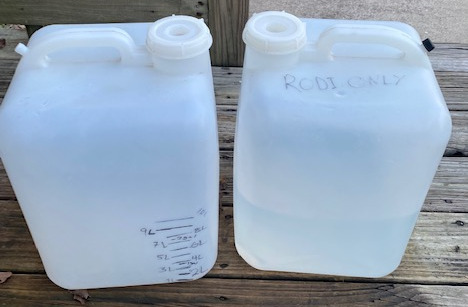
\includegraphics[width=0.8\textwidth]{Jugs.jpg}
    \caption{The two 5-gallon jugs. One has liter markings, and the other is exclusively for RODI water}
\end{figure}

Lastly, RODI filter get slightly faster at producing water after running them for a little while. If you're making RODI water 
for a water change, try to have the "RODI ONLY" jug filled to the brim after the end of the water change to save yourself some
time down the road. 

\subsection{Warning}
RODI water is not potable. It's not toxic to drink the RODI water, but because it is lacking the electrolytes and minerals that are
naturally found in drinking water, it does not hydrate you, but actually dilutes your blood electrolytes. 

\newpage
\section{Making the RODI Water}
\begin{enumerate}
    \item If you have not yet, read the introduction. 
    \item Lay the RODI filter on the cat house. It helps if the side with the white tube is closest to the faucet.
    \begin{figure}[H]
        \centering
        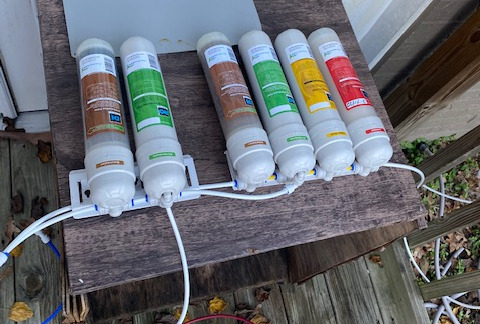
\includegraphics[width=0.8\textwidth]{RodiSetup.jpg}
        \caption{The RO/DI filter on the cat house}
    \end{figure}
    
    \item Open the valve on the red tube by pushing the handle until it is inline with the tubing. 
    \begin{figure}[H]
        \centering
        \begin{subfigure}{0.5\textwidth}
            \centering
            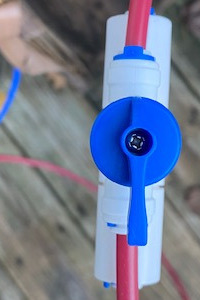
\includegraphics[width=0.9\textwidth]{ValveOpen.jpg}
            \caption{Open Valve}
        \end{subfigure}%
        \begin{subfigure}{0.5\textwidth}
            \centering
            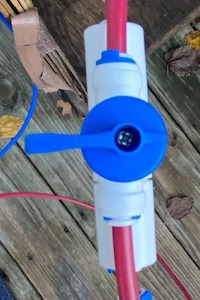
\includegraphics[width=0.9\textwidth]{ValveClosed.jpg}
            \caption{Closed Valve}
        \end{subfigure}
        \caption{The Red Line's Valve}
    \end{figure}
    
    \item Wedge the red tube's end between the slats in the porch. 
    \begin{figure}[H]
        \centering
        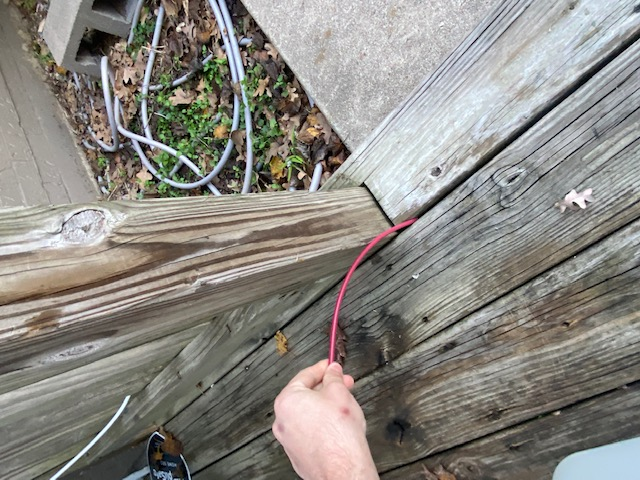
\includegraphics[width=0.5\textwidth, angle=-90]{RedLineDrain.jpg}
        \caption{The drain line wedged into the porch slats}
    \end{figure}

    
    \item \textbf{Do not place the blue tube in the water container yet}

    \item Connect the white tube to the faucet. The tube has a normal garden hose adapter, but is a little difficult to screw
    in.
    \begin{figure}[H]
        \centering
        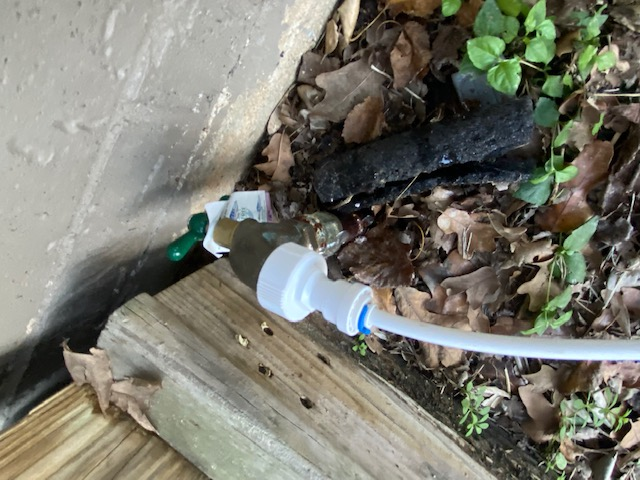
\includegraphics[width=0.4\textwidth, angle=-90]{WhiteLine.jpg}
        \caption{The white tube connected to the faucet}
    \end{figure}
    
    \item Turn the faucet on as high as it will go.
    \item You should hear a crackling sound as the RODI filter is filled and all the air bubbles are pushed out.
    \item Once all the crackling has stopped, close the valve on the red tube by turning the handle until it is perpendicular
    to the tubing.
    \item Watch the blue tube's output. It will start off as an intermittent dribble, but the flow should stabilize. 
    \item Once the output has stabilized, put the blue tube into the water container of your choice.
    \begin{figure}[H]
        \centering
        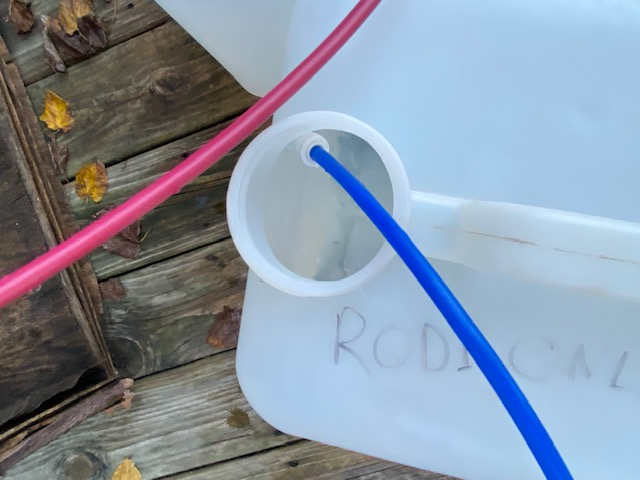
\includegraphics[width=0.4\textwidth, angle=-90]{BlueLine.jpg}
        \caption{The blue tube in the RODI container}
    \end{figure}
    
    \item Let the system run. It'll take a little while -- around an hour.
\end{enumerate}

\section{Putting up the RODI Filter}
\begin{enumerate}
    \item Turn off the faucet and unscrew the white tube
    \item Remove the blue tube from water container, if not already done (remember to close the container!)
    \item Open the valve on the red tube
    \item You should either wait for the red tube to completely drain (this'll take a while), or helicopter the end of the 
    red tube like a madman. As stupid as this makes you look, it literally pumps all the remaining water out of the tube. 
    Do this until the helicoptering stops producing water. Remember to stand clear of the tube's arc, or you'll get wet. 
    \item Fold up the two halves of the filter into each other so that the two wall mounting plates are facing each other. 
    \item Place the folded up filter back into the Athleta bag. 
    \item Roll up the tubes and wedge them into the bag. Doesn't have to look good.
\end{enumerate}

\newpage
\chapter{Freshwater 10 Gallon Tank}
\section{Aquatic Life}
\begin{figure}[H]
    \centering
    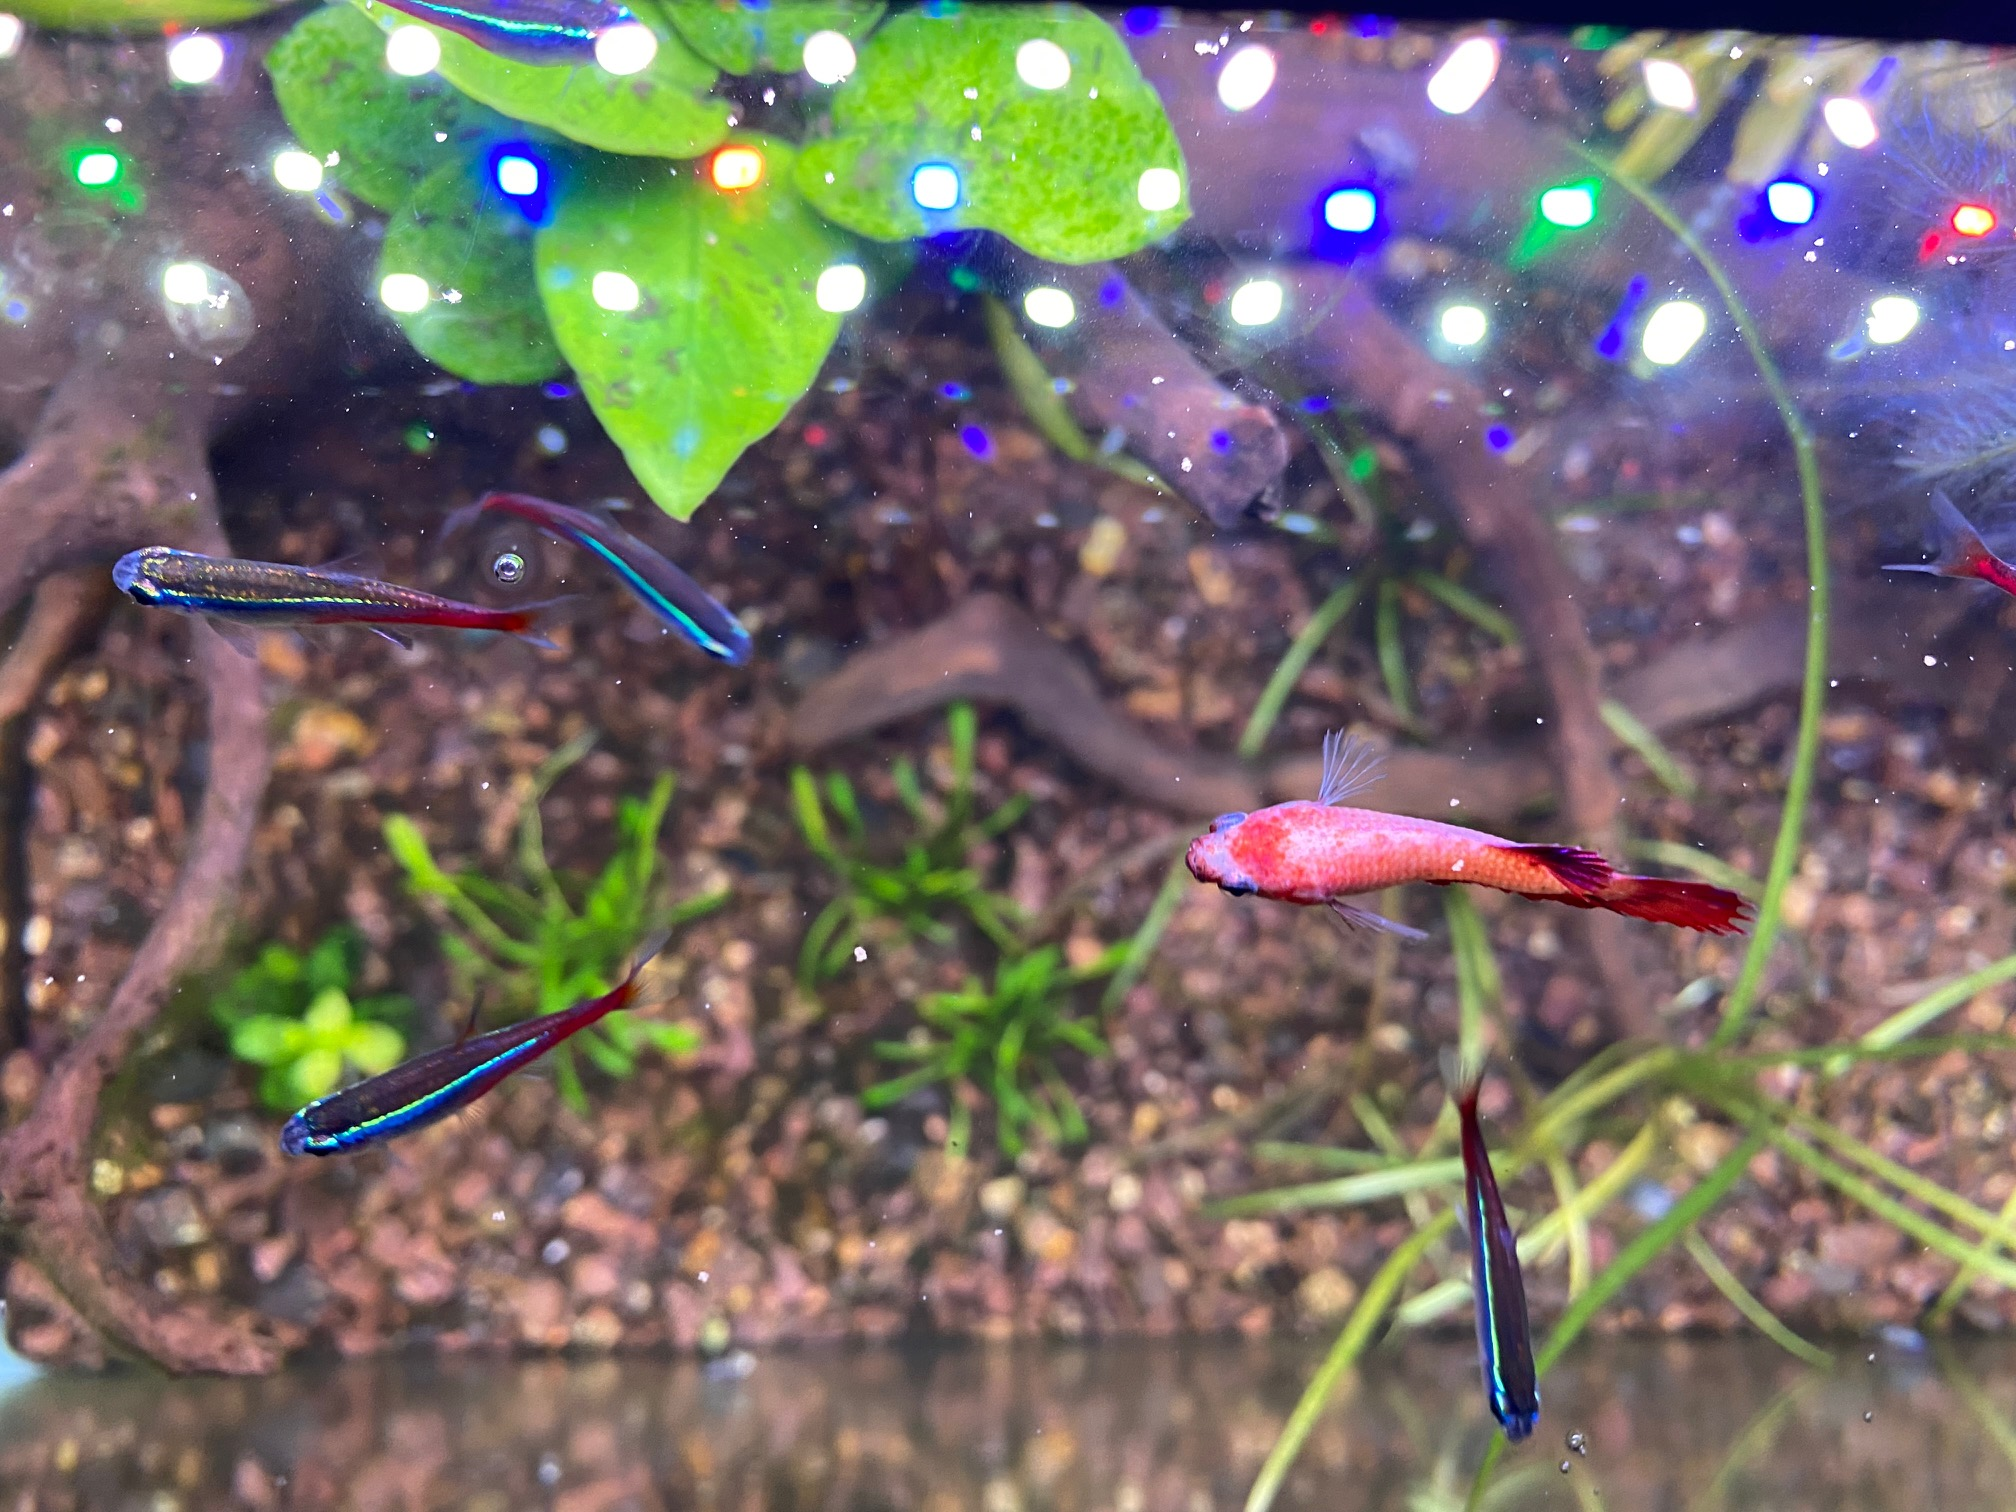
\includegraphics[width=0.8\textwidth]{GertieFocused.jpg}
    \caption{The Squad}
\end{figure}
In this aquarium we have a variety of plants and animals. Here is a list of what I know about:
\subsection{Fish Life}
\begin{itemize}
    \item \textbf{Clown Pleco}: We have 1 clown pleco. His name is Jethro and he's usually hiding under some driftwood. You 
    don't have to worry about feeding him. He eats snail eggs and driftwood and leftover fish food. 
    \item \textbf{\textit{Betta Splendens}}: We have 1 female betta. Her name is Gertie (short for Go-Gurt). She's a veritable 
    diva and loves attention. And food. Unfortunately, Gertie isn't very fast, so she needs some care and attention when 
    feeding her. 
    \item \textbf{Neon Tetras}: We have 10 neon tetras. They don't have a name because I can't for the life of me tell them apart. They are
    schooling fish and tend to be a little skittish. The are voracious eaters, so make sure the betta gets fed too.
\end{itemize}
\subsection{Plant Life}
\begin{itemize}
    \item \textbf{Amazon Sword}: front right corner of the tank.
    \item \textbf{\textit{Ludwigia Repens}}: Back right corner of the tank. Has bright magenta underleaves. If you grab a stem and 
    flip it over under the light, you'll be amazed.    
    \item \textbf{Narrowleaf \textit{Sagittaria Subulata}}: front middle of the tank. The long narrow leaves tend to catch 
    floating detritus and algae. Try to vacuum these off during water changes.
    \item \textbf{\textit{Cryptocoryne Parva}}: front left corner of the tank, next to a single stem of the Ludwigia. This is a newer plant in the aquarium. It should end up carpetting nicely. 
    \item \textbf{\textit{Anubias Barteri}}: middle left of the tank, on a a large piece of wood. 
    \item \textbf{\textit{Vallisneria Americana}}: back left corner of the tank. It grows long, helically wound leaves.
    \item \textbf{Amazon Frogbit}: Floating plant. Grows in small lilypad-like clusters.
    \item \textbf{Duckweed}: Floating Plant. There are small amoounts on the surface.
\end{itemize}

\section{Feeding}
The fish need to be fed every day, ideally. That being said, they can easily go 2-3 or more days between meals. The fish are
fed the fancy guppy pellets under the tank. Feed as much as the fish will eat in about 2 minutes. Make sure to give some
pellets to Gertie specifically, as she isn't as fast as the tetras. The pleco is nocturnal and will not eat the pellets. if the tetras a 
big and fat and are constantly floating upwards after the feeding, you've fed too much. 

\begin{figure}[H]
    \centering
    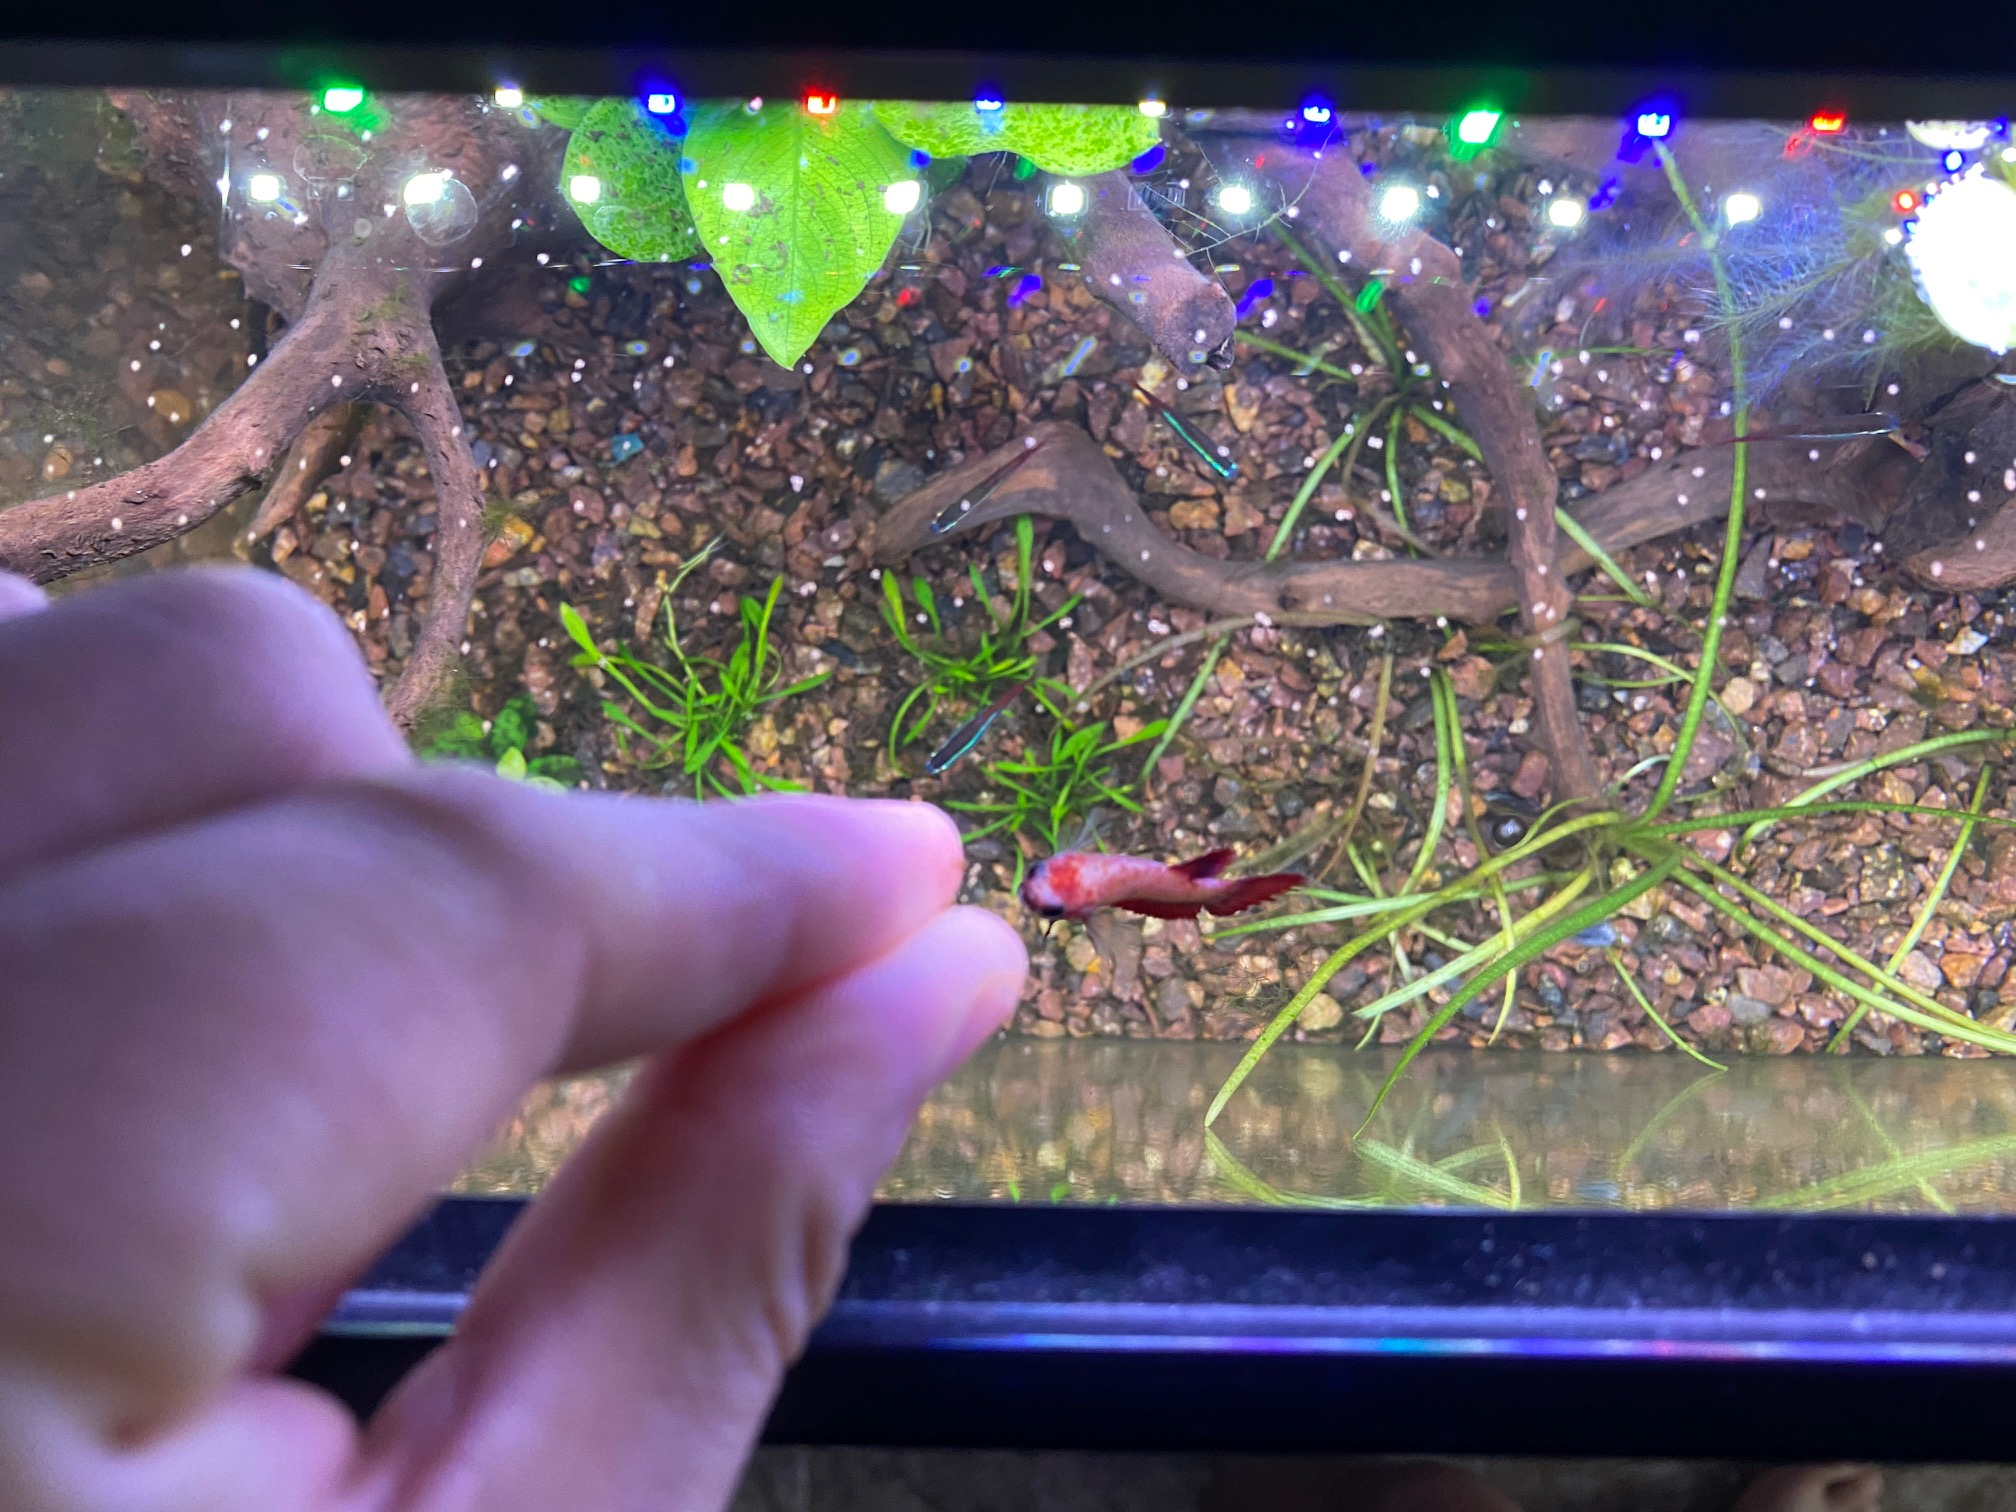
\includegraphics[width=0.8\textwidth]{FeedGertie.jpg}
    \caption{Make sure that Gertie gets her fill amidst the carnage}
\end{figure}

Once a week, you can give them enriched brine shrimp. To feed enriched brine shrimp, take the pack of shrimp out of the door
of the freezer, take a cube, and cut it into quarters with a knife. 

Get a shot glass and a pipette or syringe. Both the syringe and the pipette (which is in the refractometer box) can be found under the reef tank. Take the top-off bottle from off the reef tank and use it to fill the shot glass
about a half of the way up. Replace the top off bottle onto the tank. Melt the quarter cube in the RODI water. 

Using the pipette or syringe, slowly drop shrimp into the aquarium. Make sure to spot feed some to Gertie. You won't have to 
feed the fish the day after this (they'll be plenty fat).

After using the pipette, rinse thoroughly with RODI water. You can take a small amount of RODI water from the reef tank's \hyperref[sec:ato]{auto top-off bottle}. The syringe can simply be rinsed by repeatedly filling it and emptying it with tank water.

\section{Fertilizing}
Sure you've fed the fish, but the plants are hungry too! After every water change, and every three days, you need to give the
plants some liquid fertilizer. Grab the box that says \textbf{Seachem Plant Pack Fundamentals}. In it is a syringe to use for
dosing the fertilizers. 

You'll notice that one bottle in the box is missing. Coincidentally, that is the bottle you need. The bottle is in the door 
of the fridge. Unscrew the cap and use the syringe to draw up 0.75 mL of the fertilizer. Place the bottle back in fridge after
use or it will go bad! Squirt the fertilizer into the output of the tanks filter to mix it well.

\begin{figure}[H]
    \centering
    \begin{subfigure}{0.8\textwidth}
        \centering
        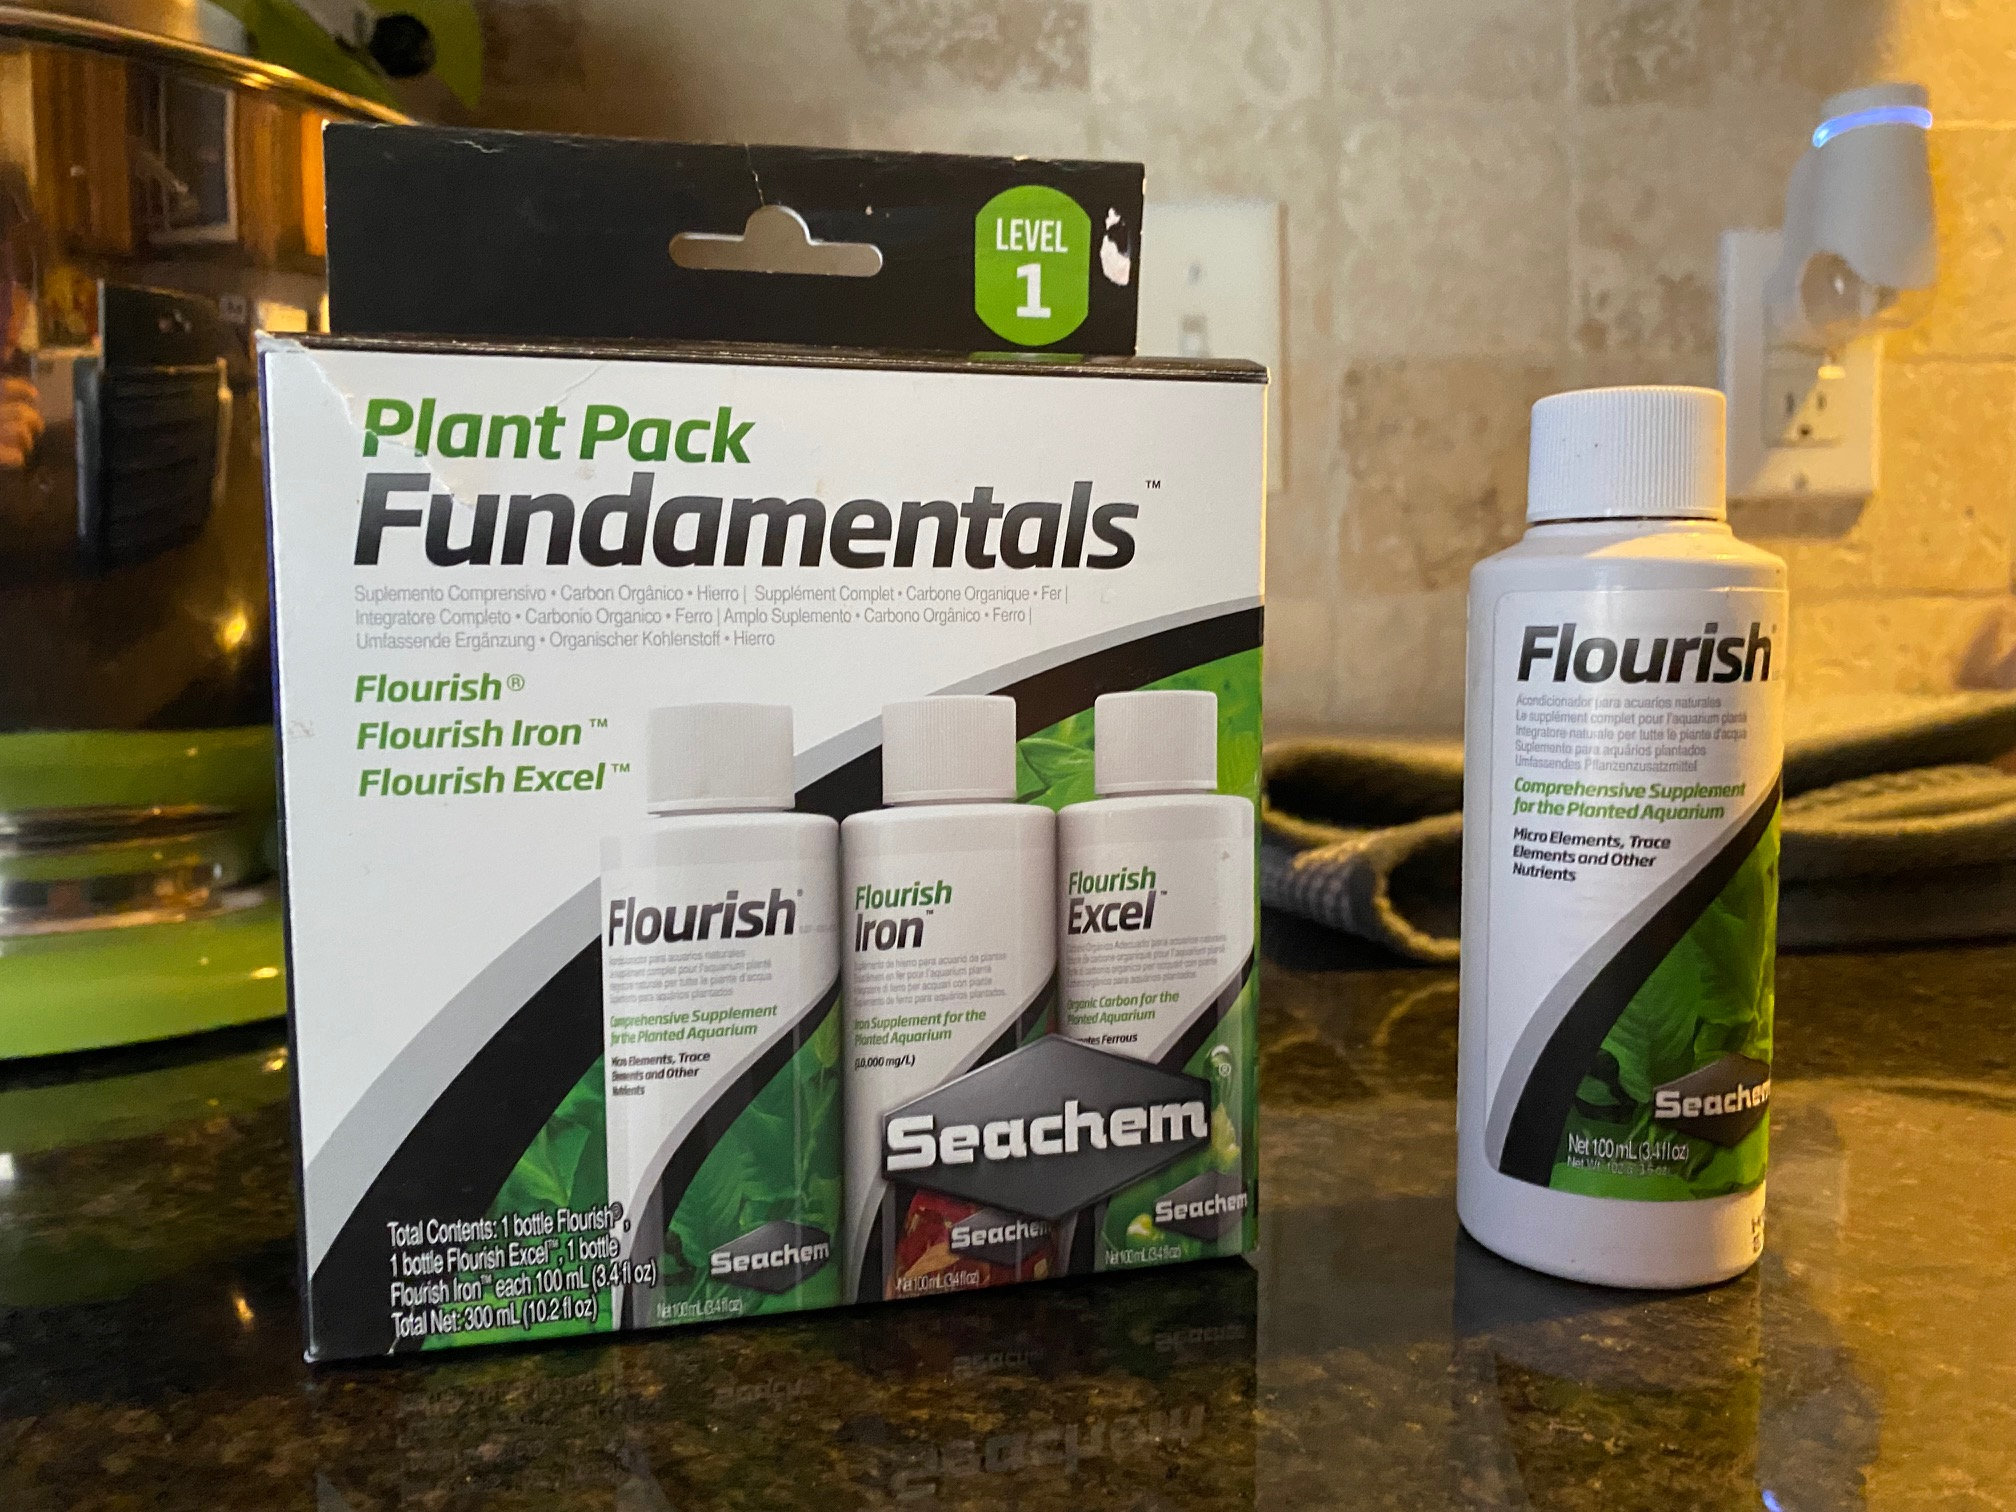
\includegraphics[width=\textwidth]{FundamentalsNFlourish.jpg}
        \caption{The Fertilizer Box and Bottle}
    \end{subfigure}
    \vfill
    \begin{subfigure}{0.5\textwidth}
        \centering
        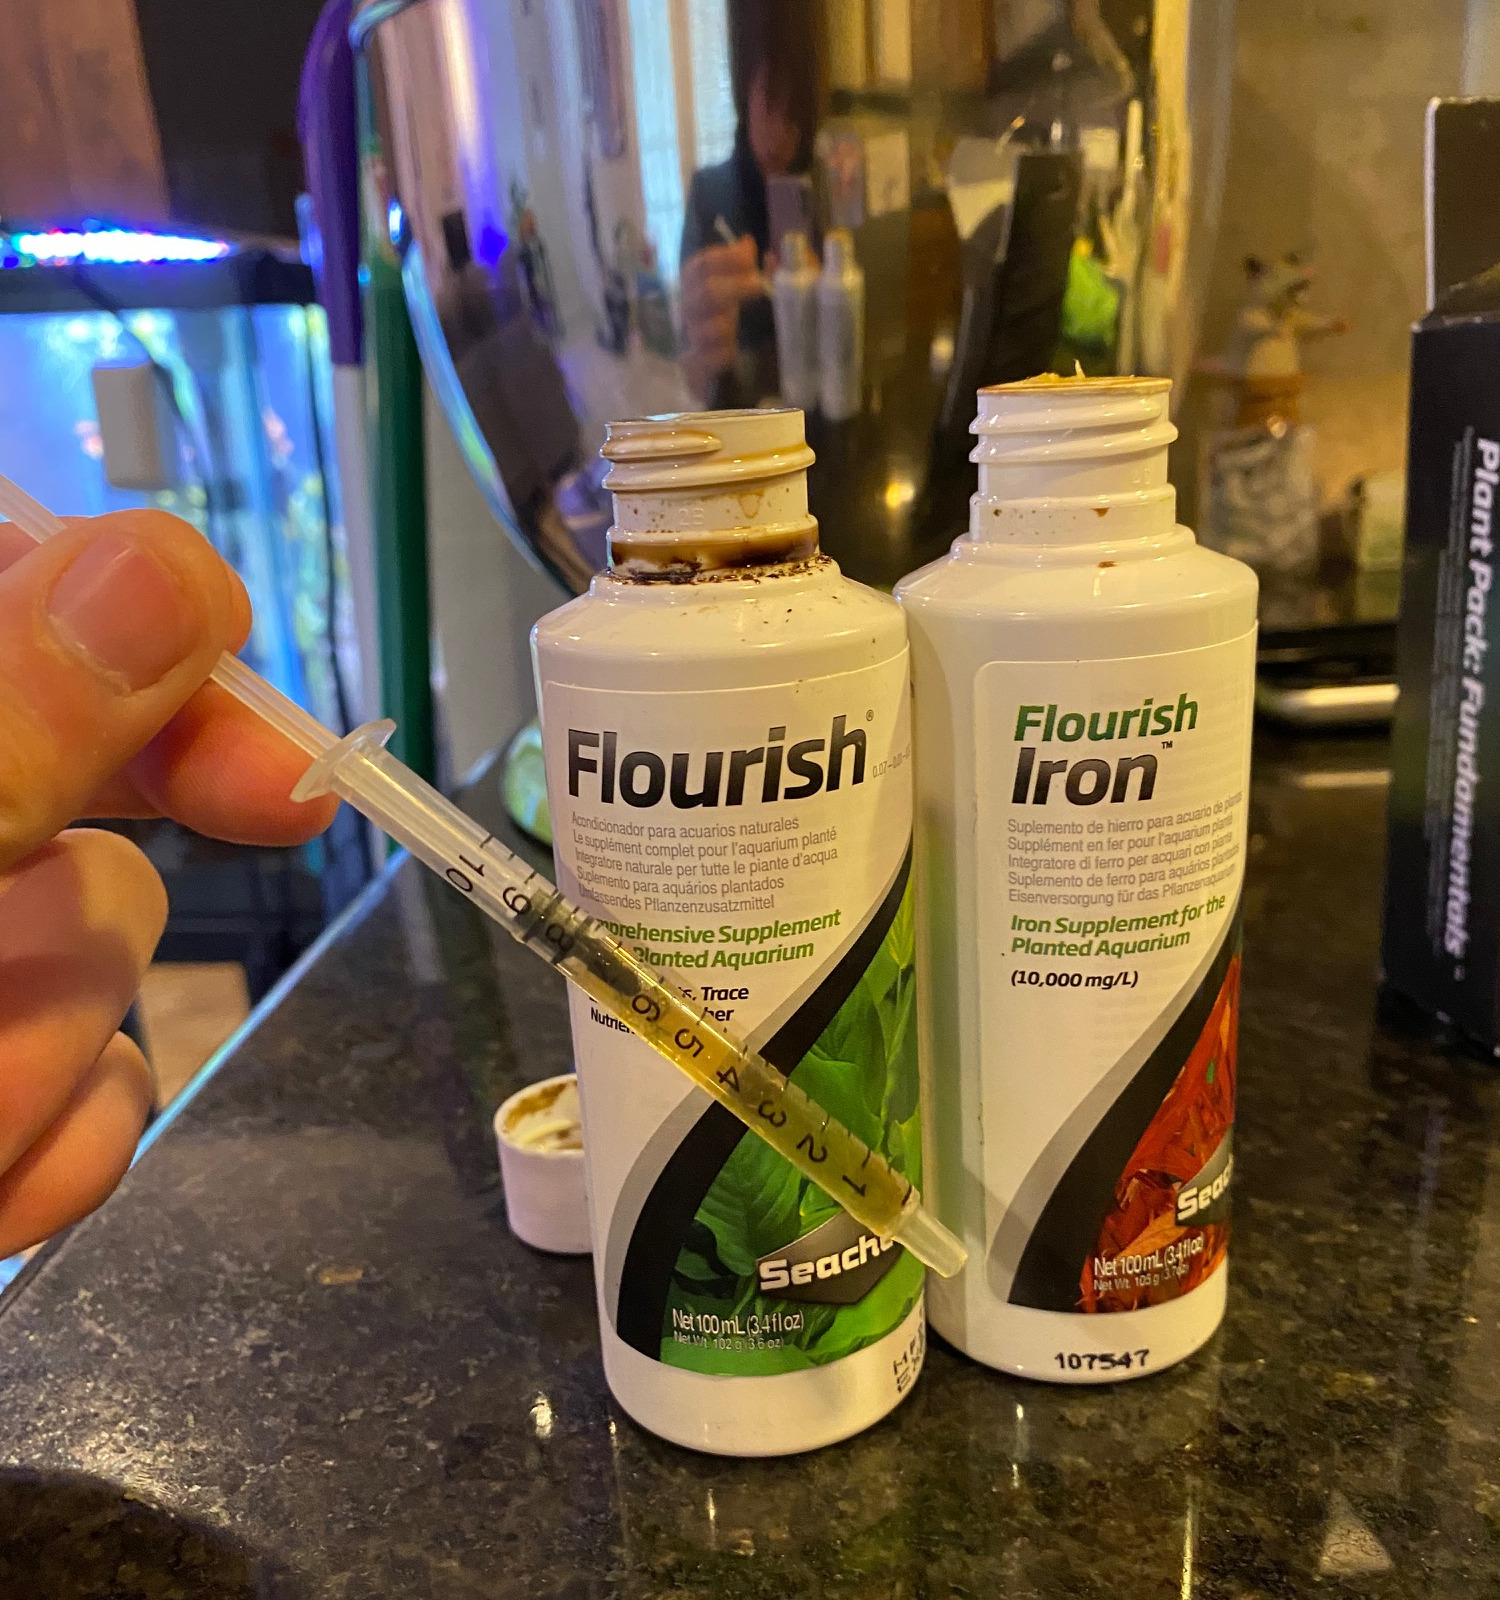
\includegraphics[width=0.9\textwidth]{FertsNSyringe.jpg}
        \caption{The full syringe}
    \end{subfigure}%
    \begin{subfigure}{0.5\textwidth}
        \centering
        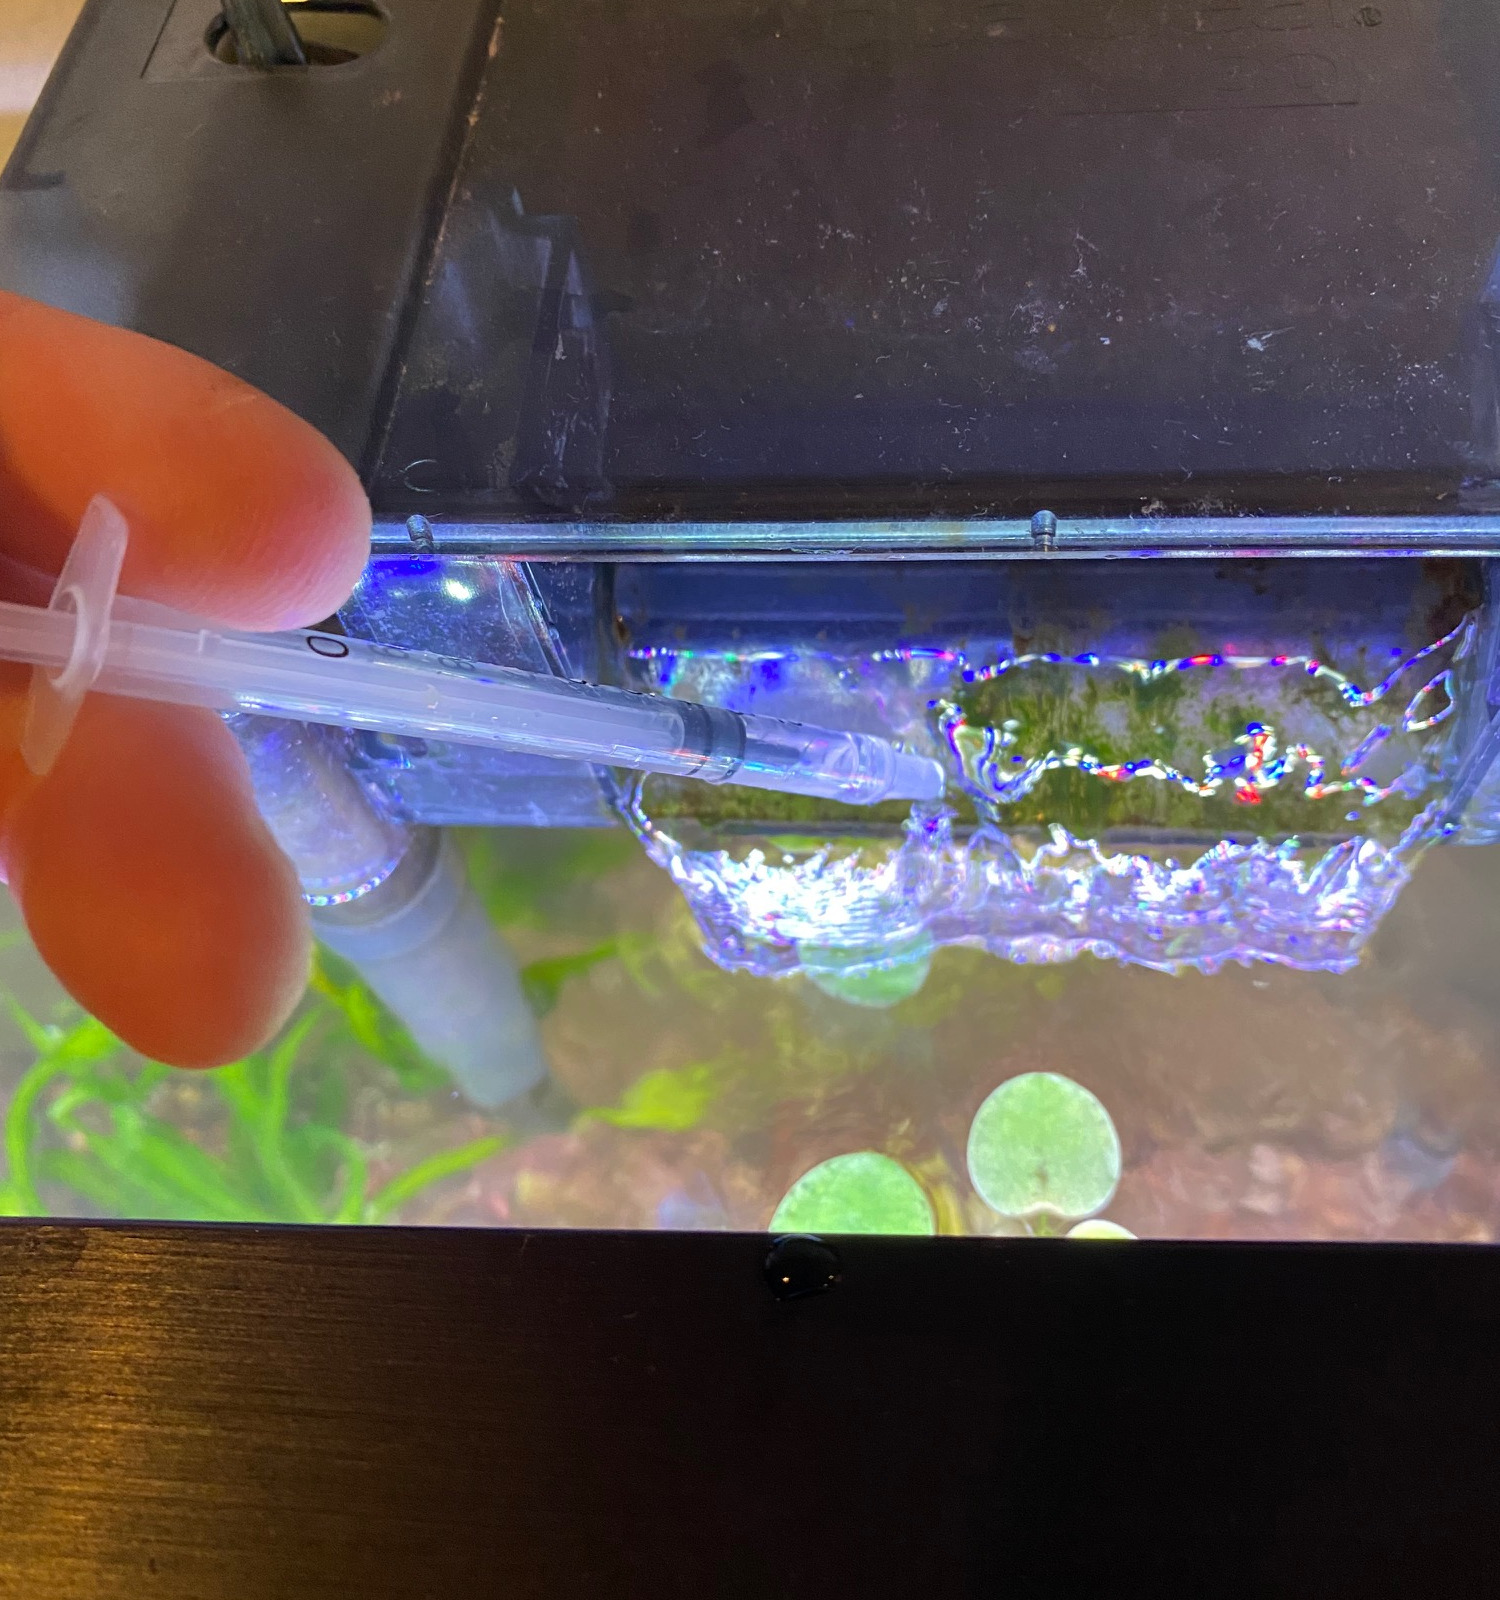
\includegraphics[width=0.9\textwidth]{FertInFilter.jpg}
        \caption{Putting the fertilizers in the tank}
    \end{subfigure}
    \caption{Fertilizing the Aquarium}
\end{figure}

After water changes, you'll additionally want to dose 1 mL of the iron supplement, in the same way that you did the normal
fertilizer. The iron supplement does not need to be refrigerated.

After using the syringe, rinse it thoroughly using tank water.

\section{Top Off}
Top off the aquarium with RODI water when it gets low. That's it.

\section{Cleaning and Maintenance}
\subsection{Water Changes}
You should change about 2.5 gallons of water per week. This amounts to a little bit more than a quarter of the tank's volume,
or about half of a 5-gallon jug. To perform a water change, thoroughly wash your hands with water, but no soap. Grab the 
hose from inside the black bucket next to the tank. The hose has a hard clear pipe attached to it. Place the end of the tube 
without the pipe in your wastewater container. Unplug the green triple plug under the tank to turn off the filter.

Dip the entire hard pipe section into the water, then lift it slightly above the rim of the tank to start the siphon. If you 
need more suction, you can pull off the hard pipe. Try to mainly remove the stubborn bits of hair algae from the bottom and 
clean the plants of accumulated detritus. You do not have to vacuum the gravel every time. Once per 2-3 weeks is a good frequency. 

\begin{figure}[H]
    \centering
    \begin{subfigure}{0.5\textwidth}
        \centering
        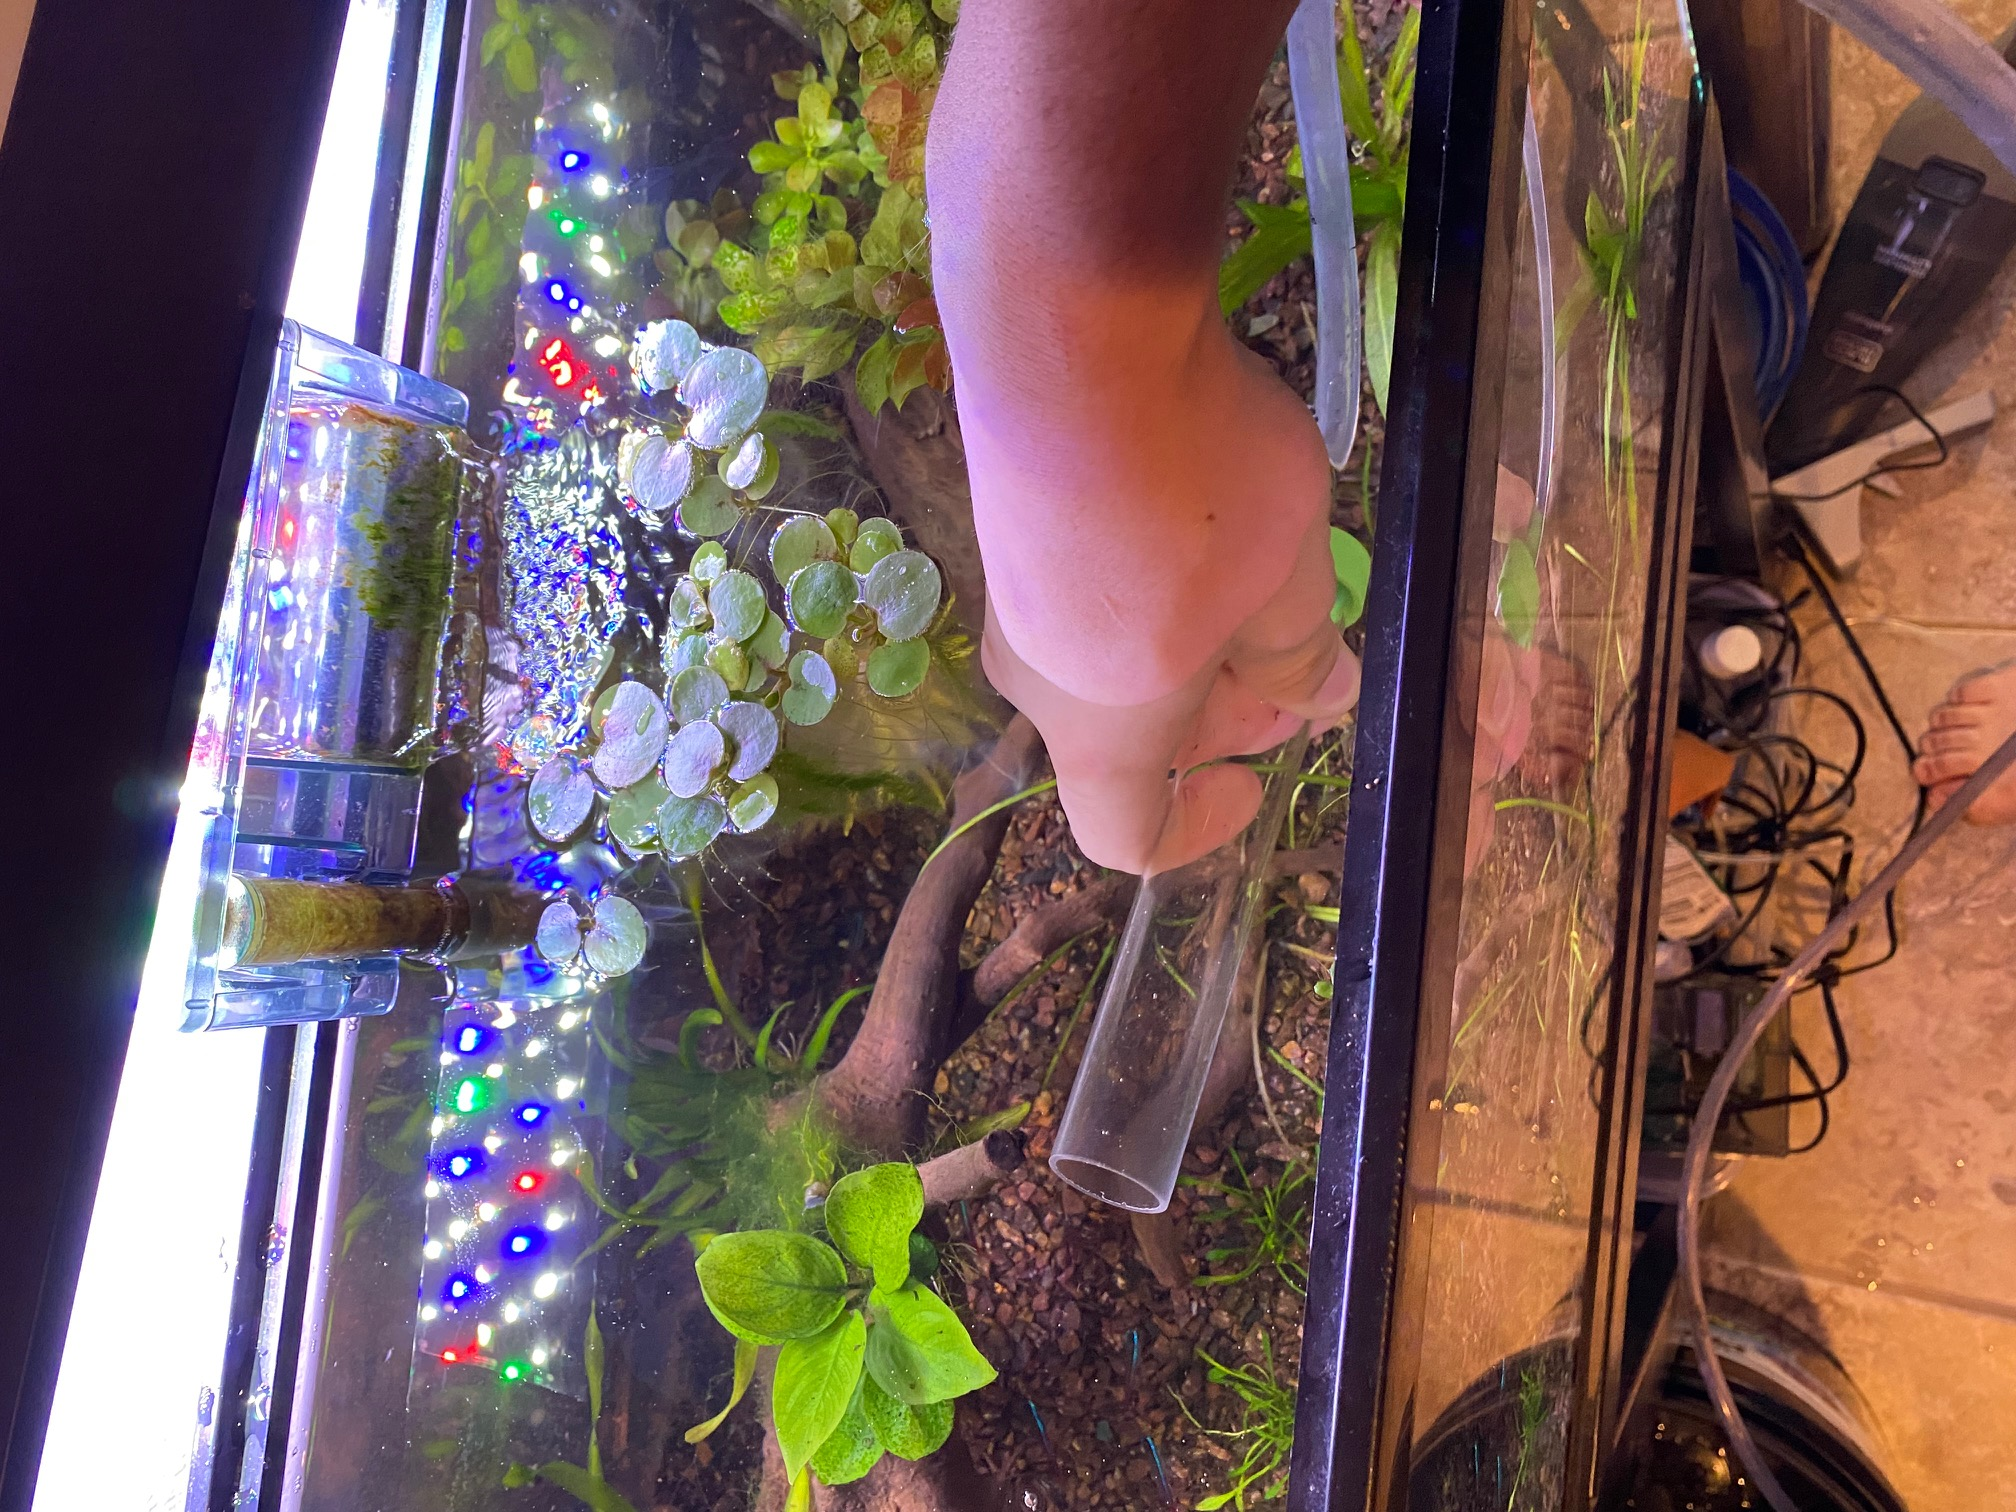
\includegraphics[width=0.9\textwidth, angle=-90]{StartSiphon1.jpg}
        \caption{Filling the pipe}
    \end{subfigure}%
    \begin{subfigure}{0.5\textwidth}
        \centering
        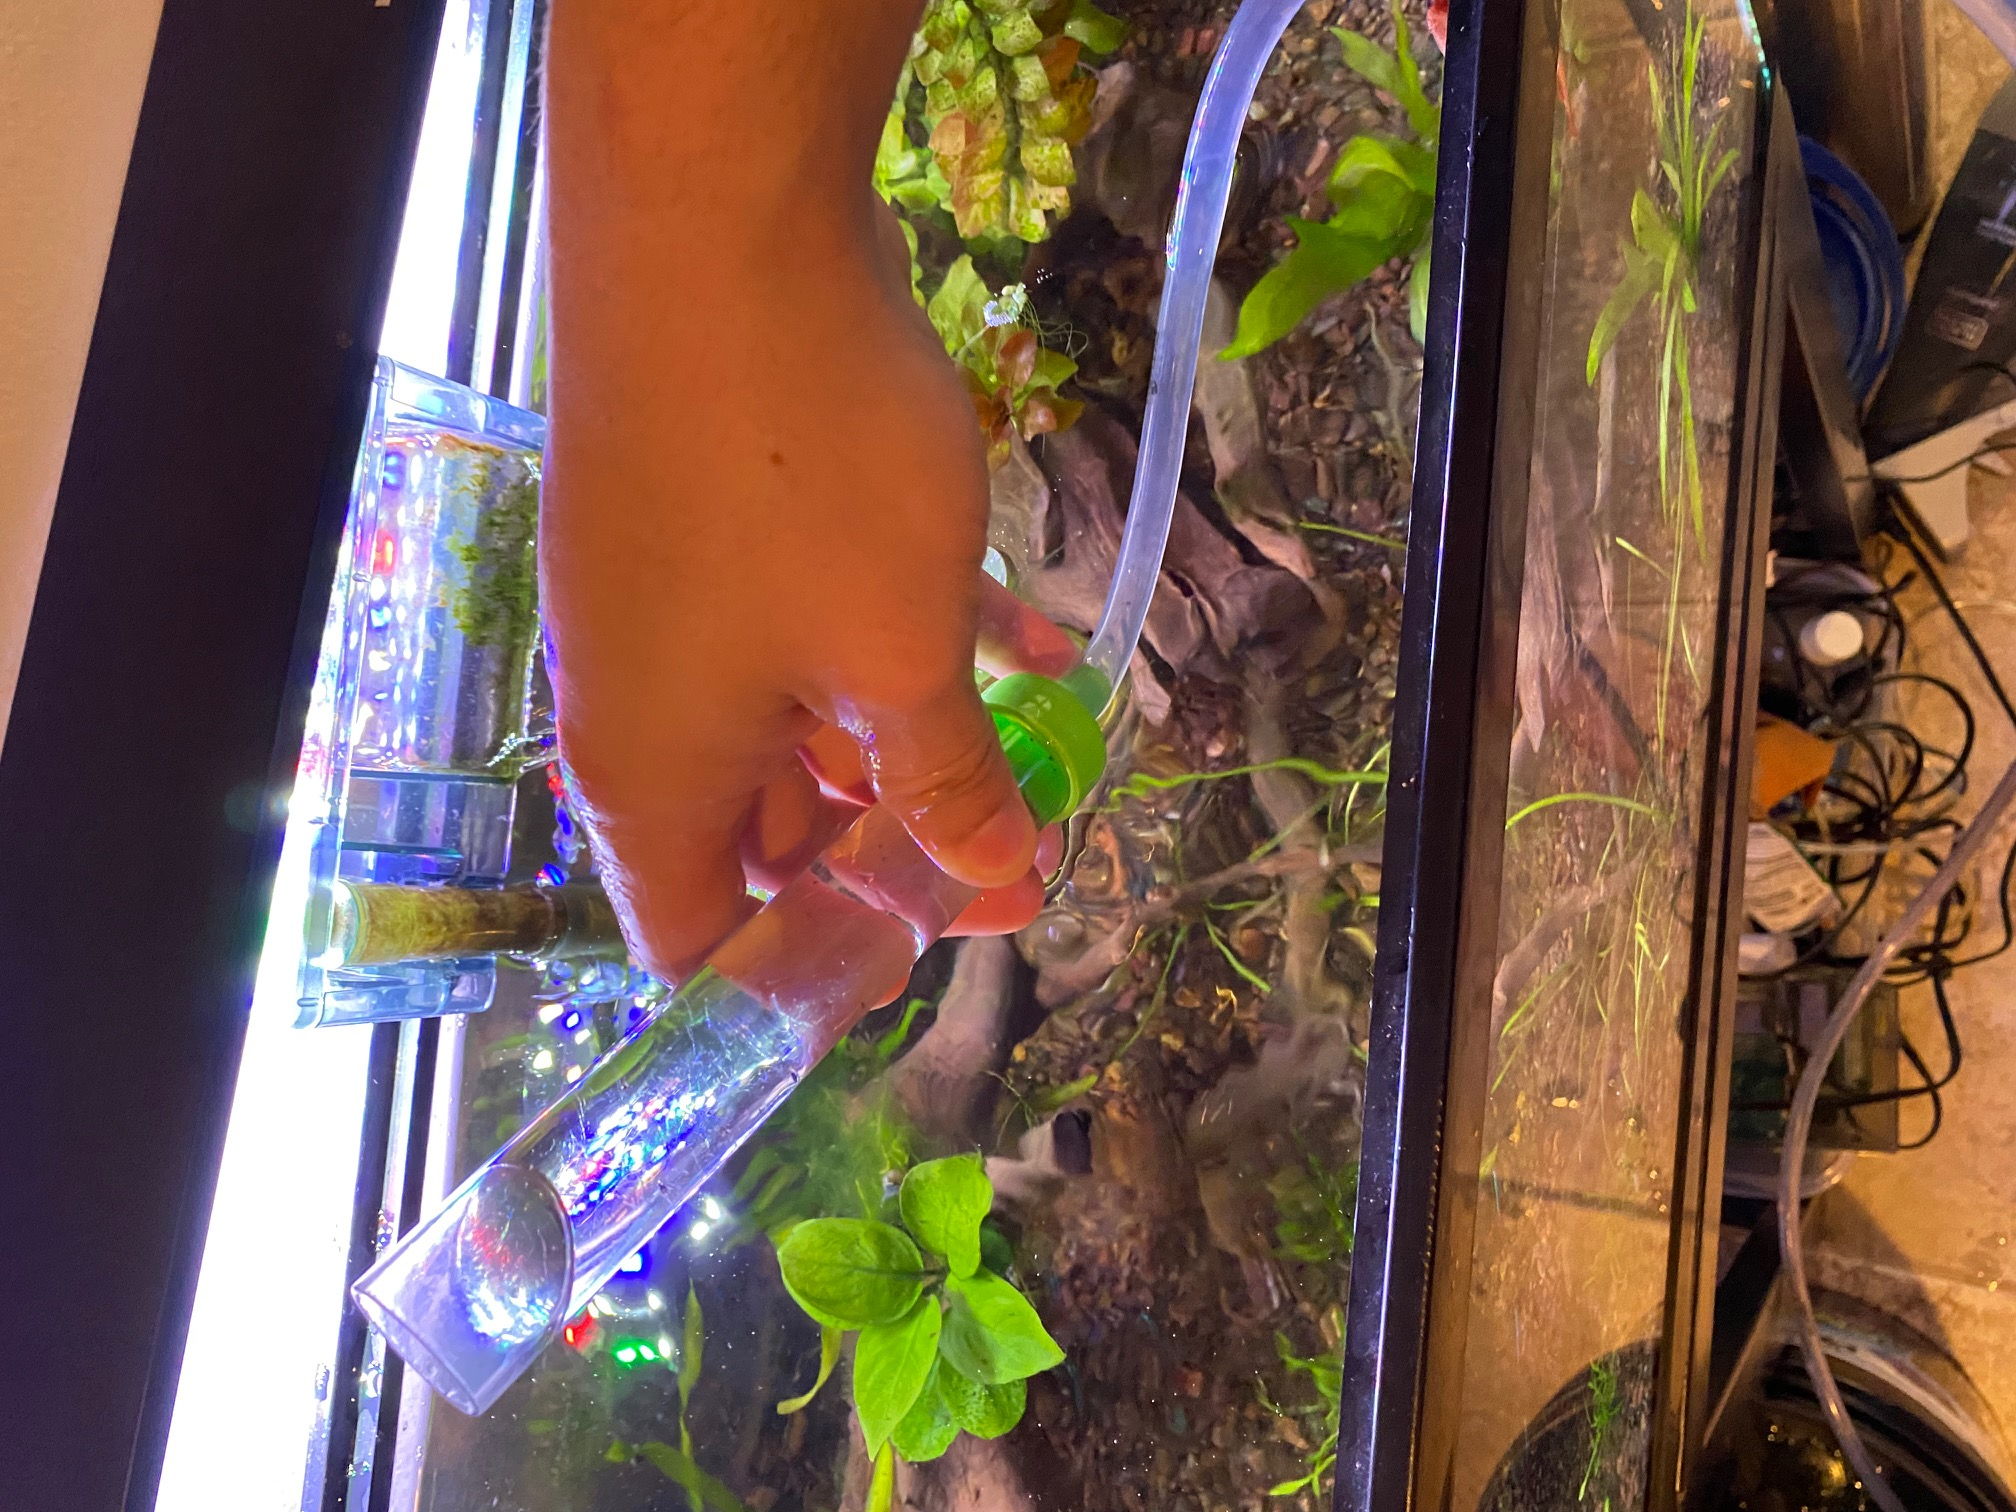
\includegraphics[width=0.9\textwidth, angle=-90]{StartSiphon2.jpg}
        \caption{Lifting the pipe}
    \end{subfigure}
    \caption{Starting the siphon}
\end{figure}

Dump the wastewater into the toilet. Follow the instructions in \hyperref[subsubsec:filtermain]{filter maintenance} before 
continuing. Refill the tank with RODI water. Splash some water into the filter box to ensure that it will start up easily. 
Plug the filter into the socket, and ensure that it fills with water.

\subsection{Filter Maintenance}
\label{subsubsec:filtermain}

To clean the filter sponge, pour about a litre of RODI water into the black bucket. Place the sponge in the bucket and 
vigorously squeeze the grime out of it. Repeat this step once more to deep clean the sponge. Place the sponge back in the 
filter.

About once a month, or whenever the filter refuses to start, the impeller needs be cleaned. Dump the water in the filter box 
into the tank or trash. Then unscrew the black motor on the bottom left of the filter to remove it. The impeller is held in 
magnetically. Use your fingers to pull it out, or gently shake it out. 

\begin{figure}[H]
    \centering
    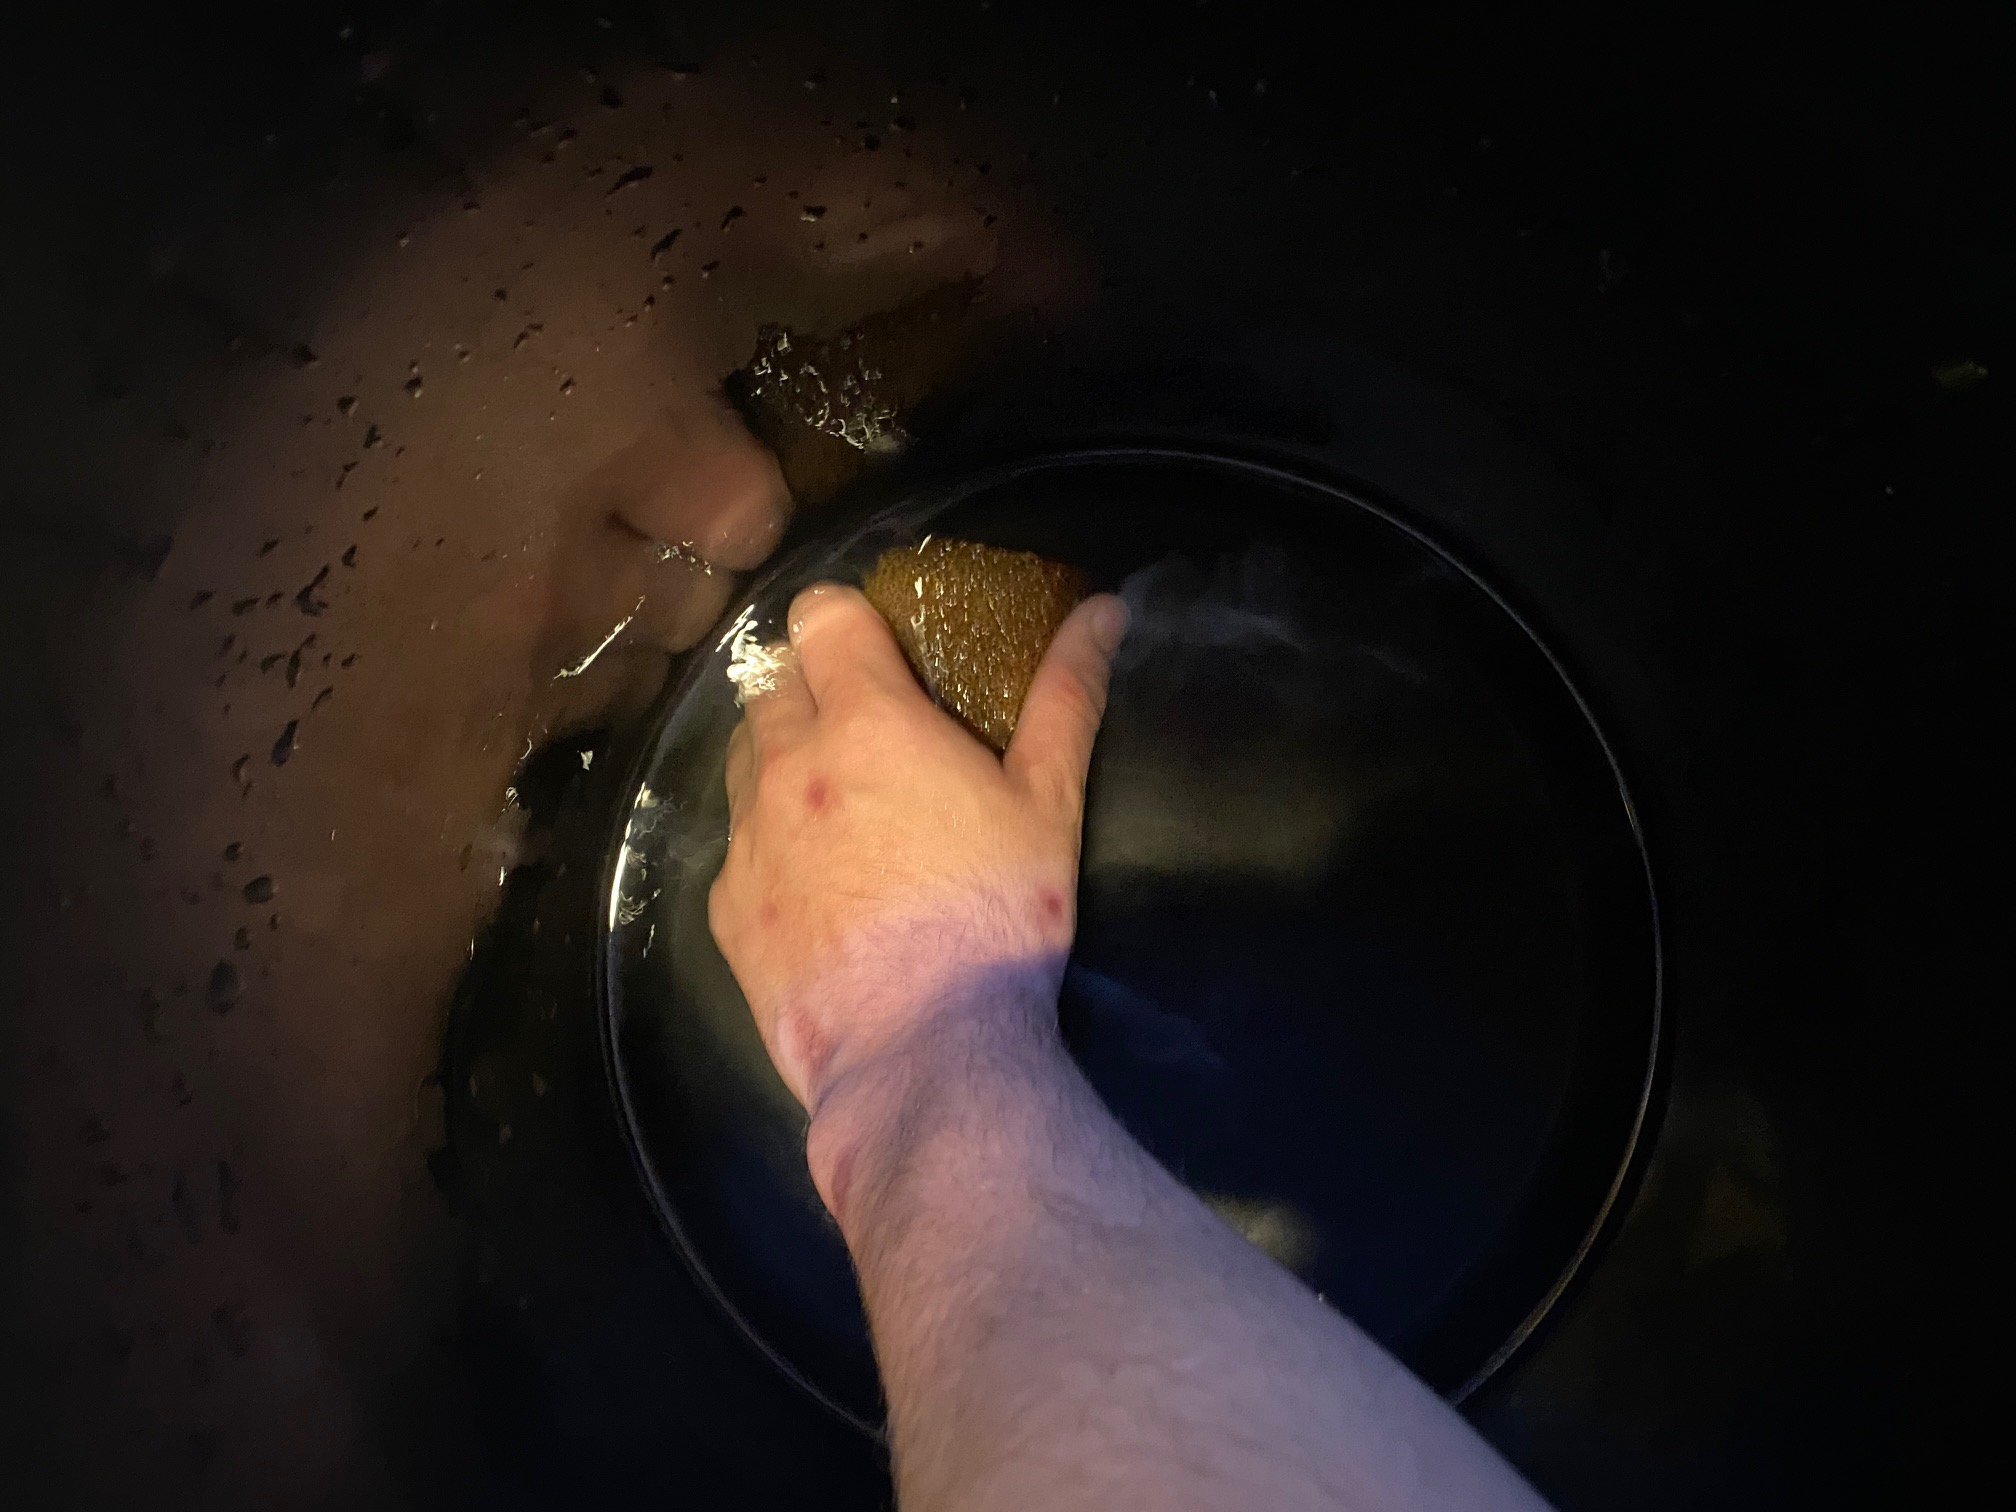
\includegraphics[width=0.8\textwidth]{CleanSponge.jpg}
    \caption{Cleaning the sponge in clean RODI water}
\end{figure}

Use a Q-tip to clean the inside of the motor. Wash the outside of the impeller under a stream of tap water. Put the impeller 
back in the motor, and screw it back into the filter. Add RODI or tank water into the filter until the impeller is covered in 
water and then plug the filter back in. It should start right up. If it doesn't contact me and I'll help you troubleshoot.

If there is algae growing on the filter's outflow ramp, brush it off with a paper towel. 

\section{Lighting}
The light on the tank is on a self timer and is already set. However, if there is a power outage, the timer will lose its
time. To fix this, press the bottom button of the light controller until the light flashes next to the current time. The time 
options are: 8:00, 10:00, 12:00, 15:00, 18:00, and 22:00. Try to set the light as close to one of these times as possible. 


\newpage
\chapter{Saltwater 12" Cube Tank}
\section{Aquatic Life}
\subsection{Fish and Invertebrate Life}
\begin{itemize}
    \item \textbf{Ocellaris Clownfish}: Cheddar is our resident goofball.
    \item \textbf{Peppermint Shrimp}: Benny is our shrimp. He'll let you feed him directly from the refractometer's pipette.
    \item \textbf{Misc. Invertebrates}: There are more small dove snails, bristle worms, and copepods than I could dream of 
    counting.
    \item \textbf{Nassarius Snail}: There is a large unnamed Nassarius snail. It is white, and usually hides in the sand. If it is out and about, it is 
    hungry.
\end{itemize}
\subsection{Coral Life}
\begin{itemize}
    \item \textbf{Bicolor Frogspawn}: Front left of the tank, with very bushy tentacles
    \item \textbf{Green Star Polyps}: Small neon green polyps encrusting on the front right of the rockwork. 
    \item \textbf{\textit{Alveopora sp.}}: Front right of the tank, behind the green star polyps. Was being eaten by the 
    emerald crab (rot in hell), so its not happy.
    \item \textbf{Red \textit{Montipora Capricornis}}: Middle of the tank. Grows in a big plate form.
    \item \textbf{\textit{Micromussa Lordhowensis} "Acan"}: Rear right of the tank. Big dome consisting of green disks with a 
    white circle and a ton of short tentacles sticking out. Constantly hungry. 
    \item \textbf{Green \textit{Montipora Digitata}}: Middle of the tank. Grows like a bunch of green fingers.
    \item \textbf{\textit{Acropora sp.}}: Top left, growing up towards the light.
    \item \textbf{\textit{Acropora Millepora}}: Middle of the tank. Grows as a stick pointing straight toward the front glass.
    \item \textbf{Birdsnest}: Back of the tank branching coral. Is unhappy with me, but I really don't know why. I think the 
    crab (RIH) was eating it. 
\end{itemize}
\section{Feeding}
To feed, pause the pump by pressing the "speed/feed" button on the pump controller until the pump turns off. You can also 
unplug the pump, but don't forget to plug it back in!

Every day, feed as much as Cheddar will eat in about 2 minutes. Feed Cheddar by grasping not more than 3-5 pellets from the 
fish food, and dropping them into the tank from about 8 inches above the water. This ensures that the pellets will sink, 
which helps Cheddar eat. You need to feed about 50\% more food than what Cheddar will eat so that the other animals have 
enough to eat. 

When you feed the freshwater fish brine shrimp, you can also feed the reef tank brine shrimp. Fill the shot glass half full 
with tank water and add a quarter cube of brine shrimp. When it's all melted, gently use the syringe to drop brine shrimp 
into the water. If you're feeling up to it, you may also feed the acans. The syringe can be found under the tank. After use, rinse the syringe thoroughly with tank water from the freshwater aquarium.

Thoroughly wash your hands with no soap. Draw a syringeful of brine shrimp, dip your  hand into the tank with brine shrimp, 
and gently squirt shrimp into each of the acan's heads. The heads will close up while they eat. Try to feed each head 
individually. Don't be afraid to put the syringe right near the acan's mouth.

Throw away any unused brine shrimp. 

\section{Top Off}
\label{sec:ato}
The aquarium has a bottle sticking out the top of it. This bottle keeps the salinity in the aquarium stable by refilling the aquarium the moment that the water level gets too low. Keep this bottle filled as much as possible. Ideally, check the water level every time you feed the fish. Once the bottle is half empty, refill it. 

The bottle is attached to a tripartite contraption which holds it onto the tank. The three parts are a white plastic holder which forms the structure of the auto top-off (ATO), a clearish adapter which screws into the bottle and into the white plastic structure, and an insert in the legs of the structure which grips the tank's walls. 

There are two ways to refill the bottle: using the water change hose, or using a measuring cup. The hose can be found in the black bucket. Put the RODI container on the table or counter, and put one end of the hose in the water. Suck on the other end to start the siphon, and fill your bottle. Remember to put the hose back in the bucket. 
\section{Cleaning and Maintenance}
Moreso than for the freshwater aquarium, water changes are key to the reef tank's success. The steps described here should be 
followed carefully to ensure that the water changes are done well. Aim to perform an 8-Liter water change once a week.

\subsection{Water Preparation}
\label{sec:waterprep}
Water preparation is the most important part of the water change. It must be the same salinity as the current saltwater to 
prevent damage to the corals. Water preparation can be done up to a day in advance, as long as the saltwater bucket is kept 
closed. 

\begin{enumerate}
    \item Ensure that you have at least 9 Liters of RODI available. If not, follow the instructions in the \hyperref[sec:rodi]{RO/DI chapter}.
    \item Bring the salt bucket to the kitchen. Grab the digital scale and either a bowl or a measuring cup.
    \item Tare out the weight of the cup or bowl on the scale.
    \begin{figure}[H]
        \centering
        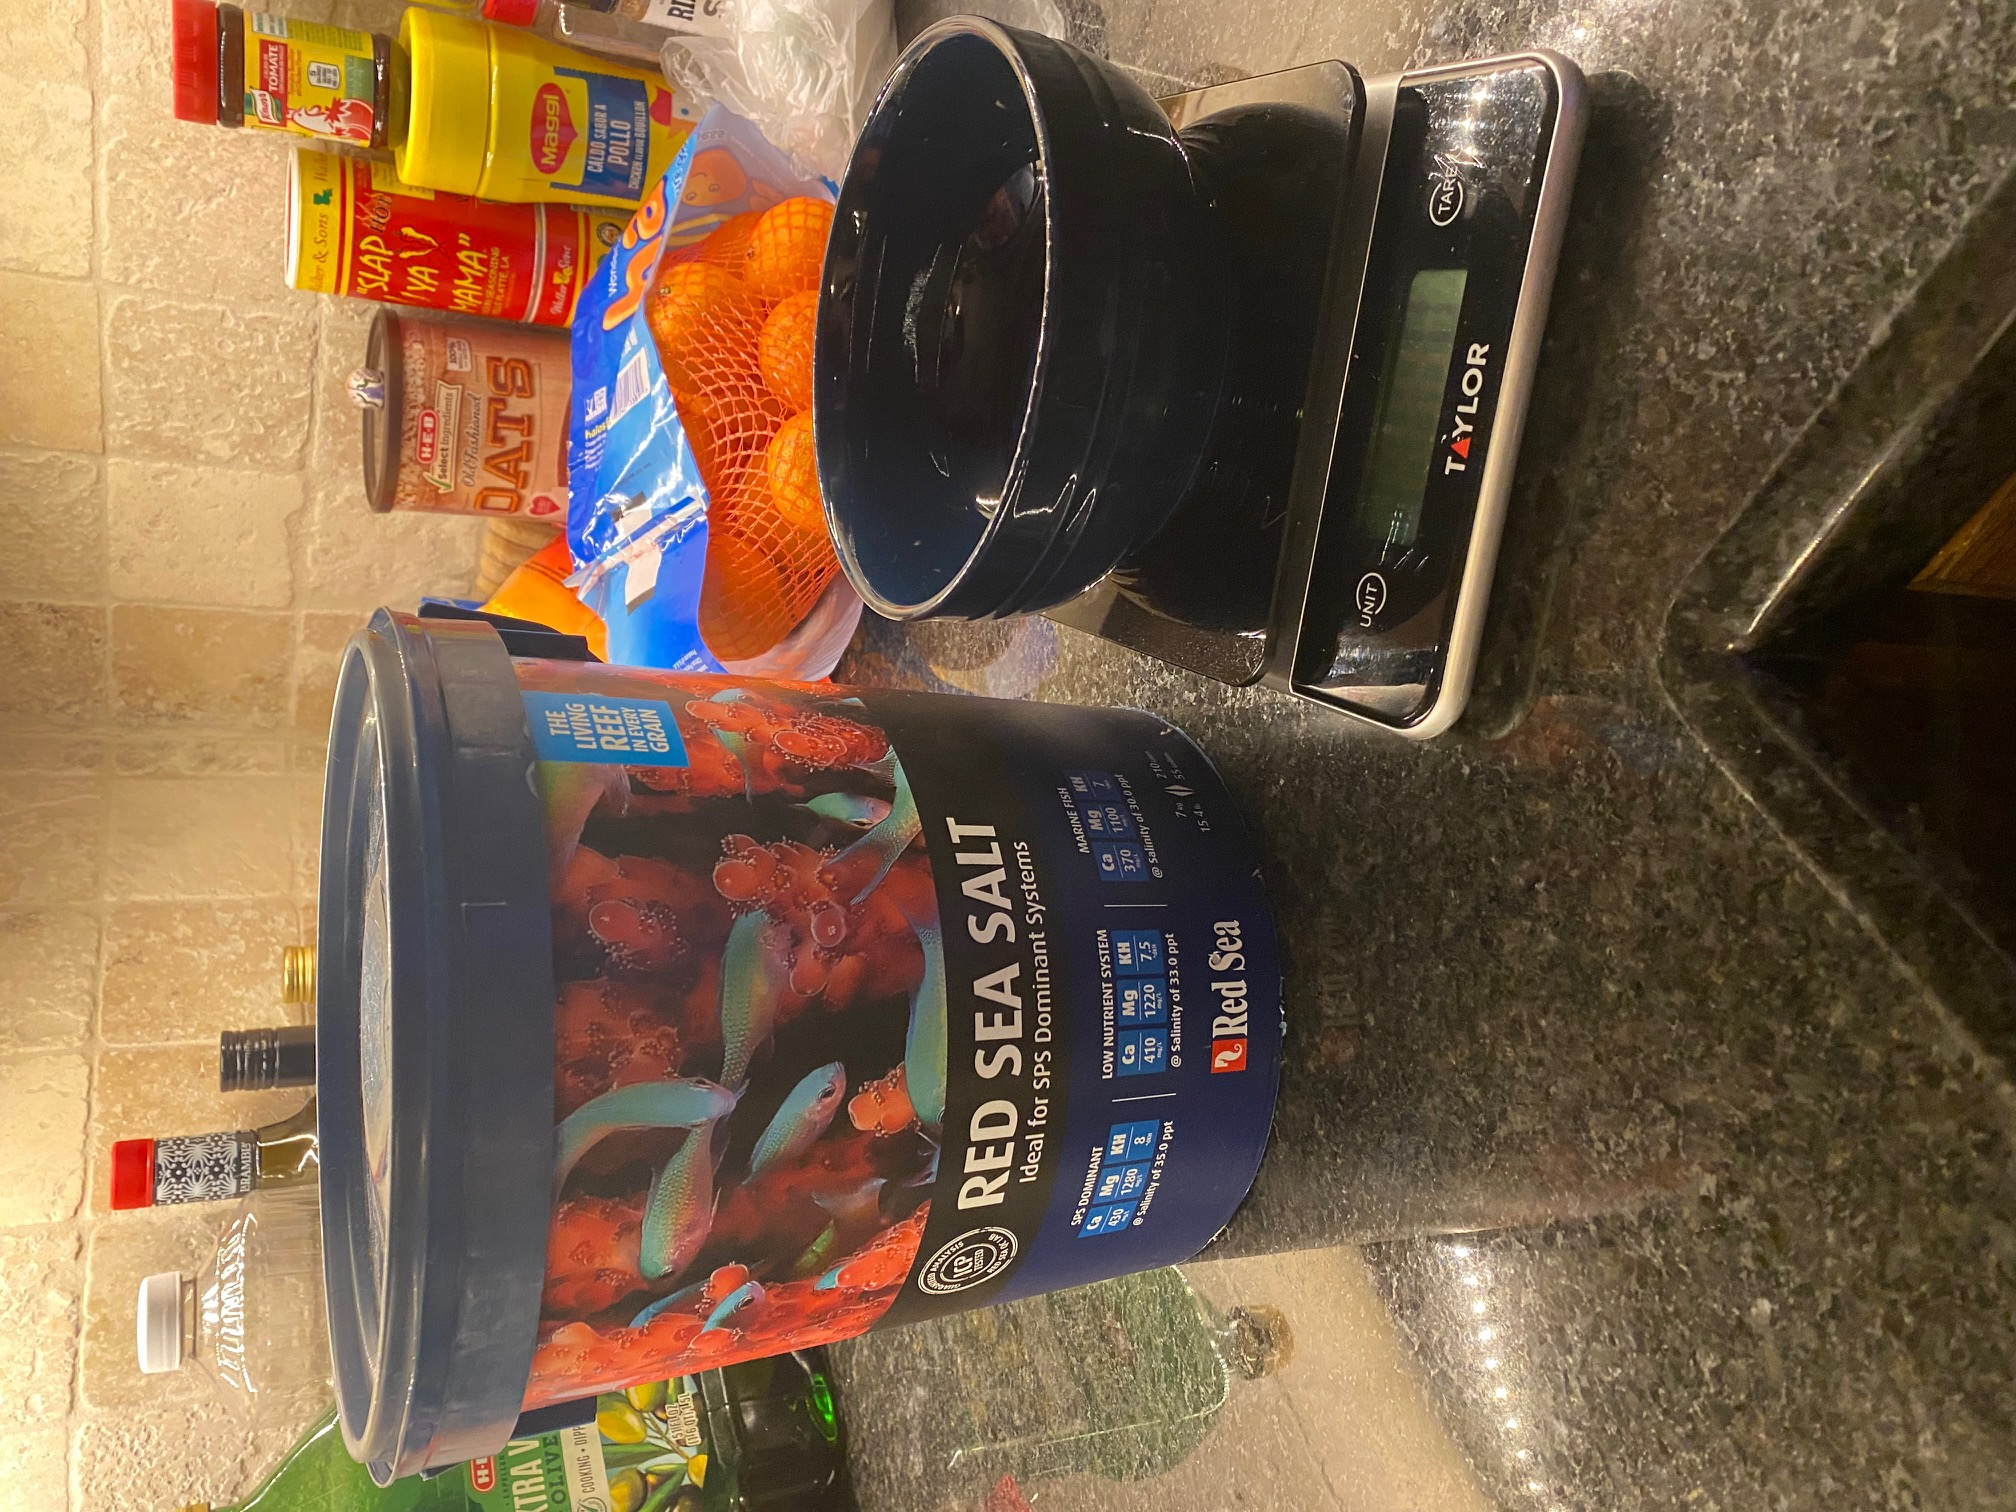
\includegraphics[width=0.5\textwidth, angle=-90]{SaltNScale.jpg}
        \caption{Salt bucket and a tared bowl}
    \end{figure}
    
    \item Measure out $315\pm5$ grams of salt.
    \item Rinse out the black bucket with some RODI water.
    \item Measure out 8 Liters of RODI water using the jug with measurements on it.
    \begin{figure}[H]
        \centering
        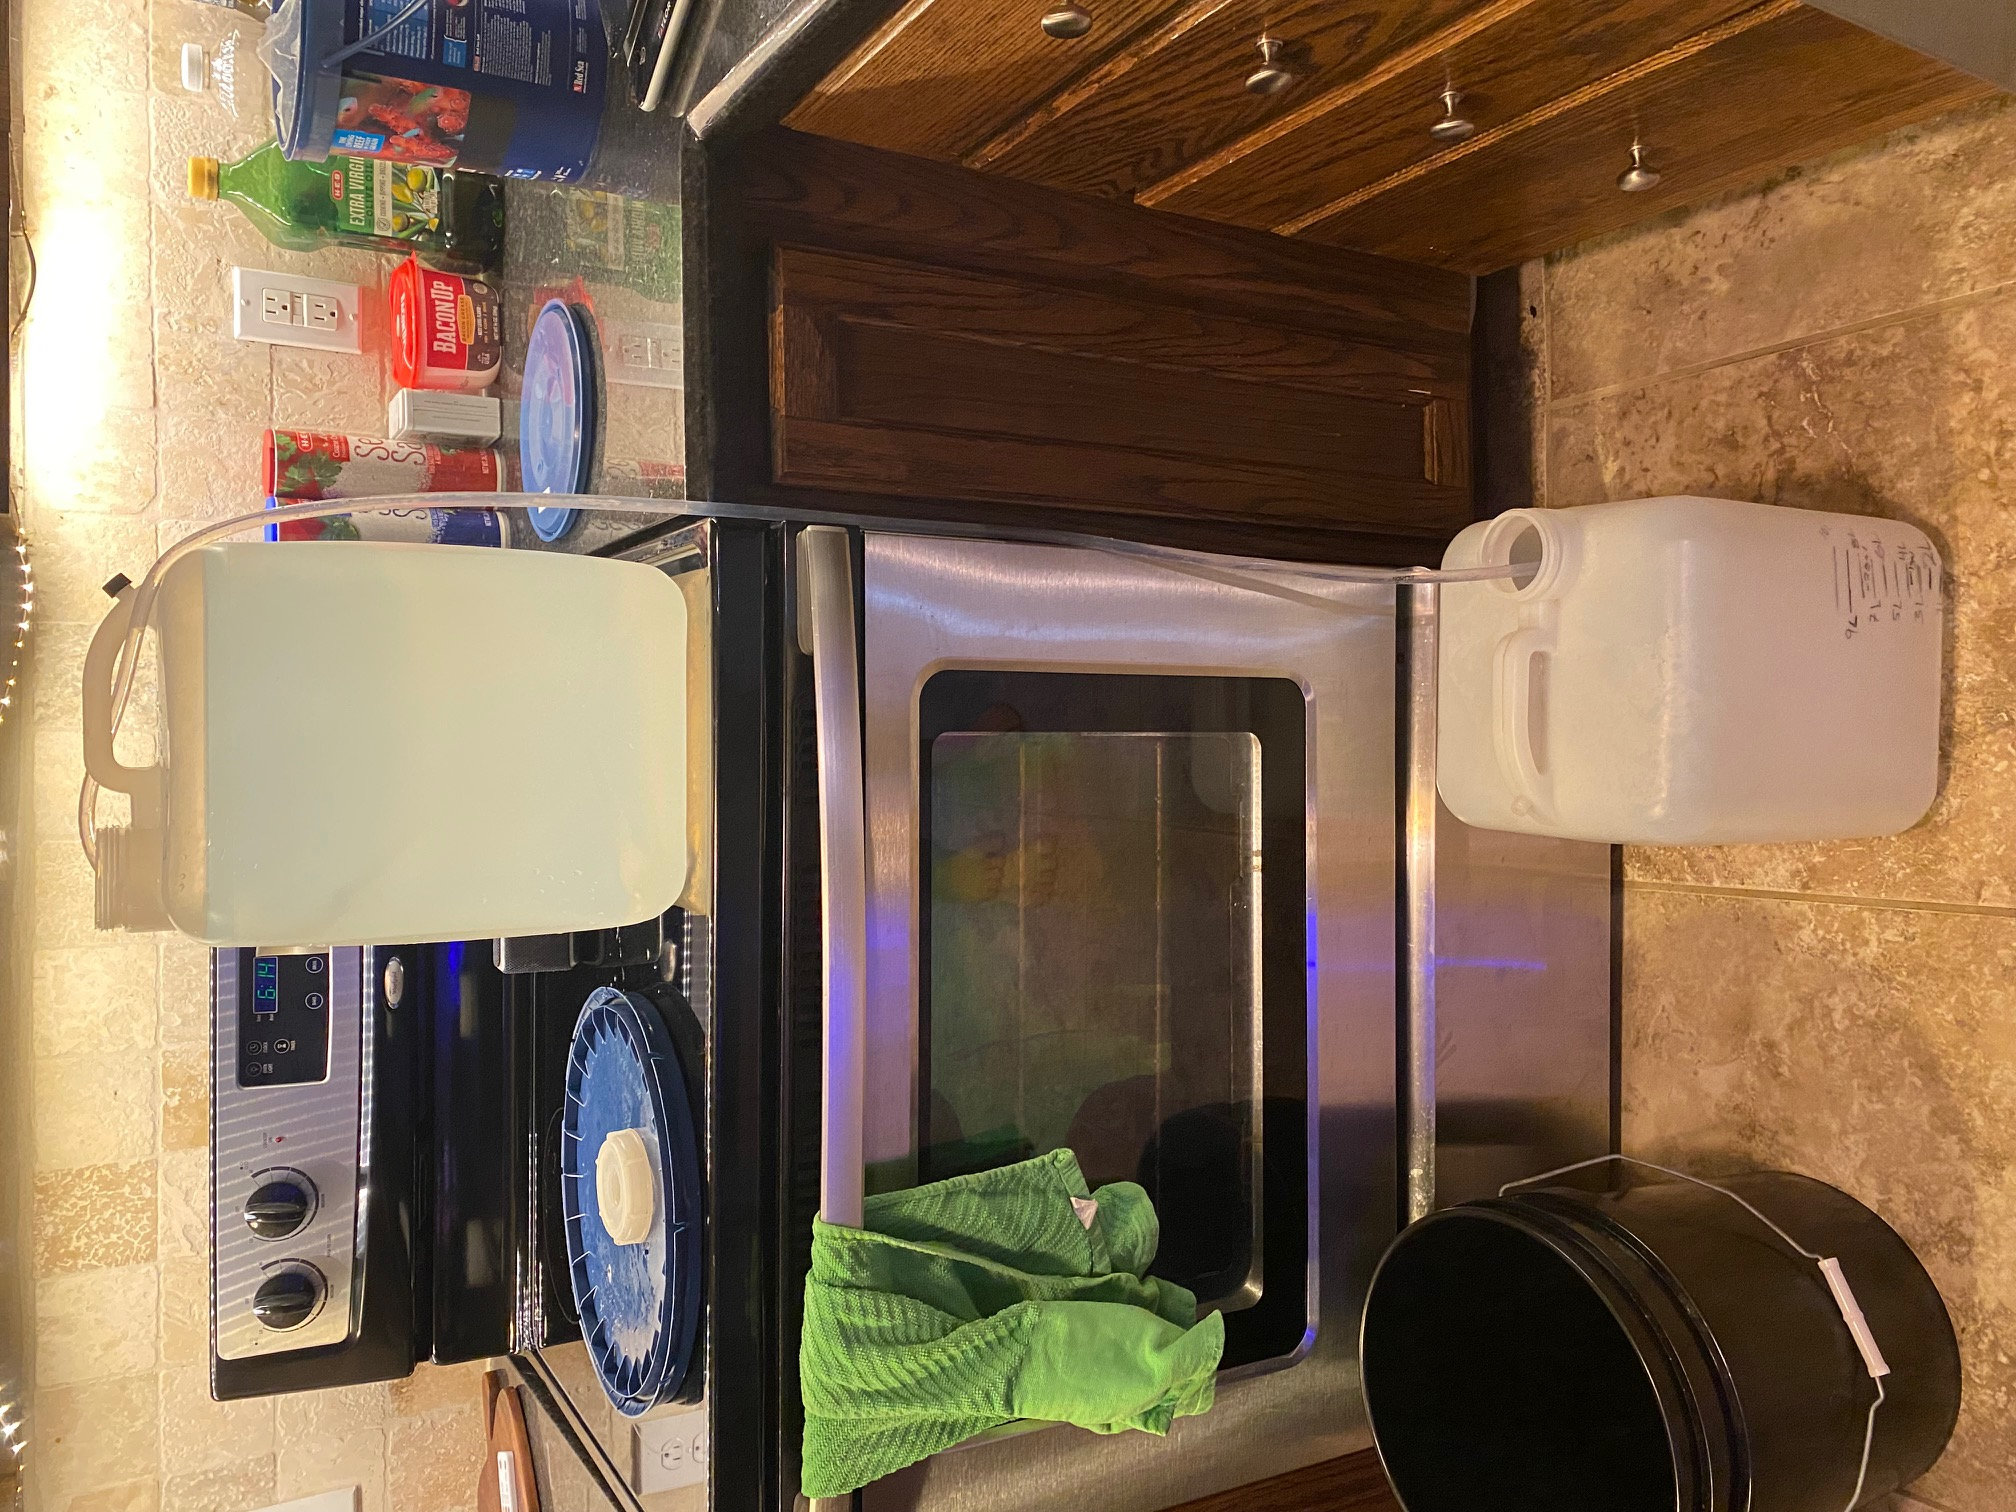
\includegraphics[width=0.5\textwidth, angle=-90]{FillingTheJug.jpg}
        \caption{Filling the jug using the water change hose}
    \end{figure}
    
    \item Pour the 8 Liters in the black bucket, along with the salt.
    \item Stir the water in the bucket with a clean utensil
    \item Wait until the water is completely clear before using it or testing it.
    \begin{figure}[H]
        \centering
        \begin{subfigure}{0.5\textwidth}
            \centering
            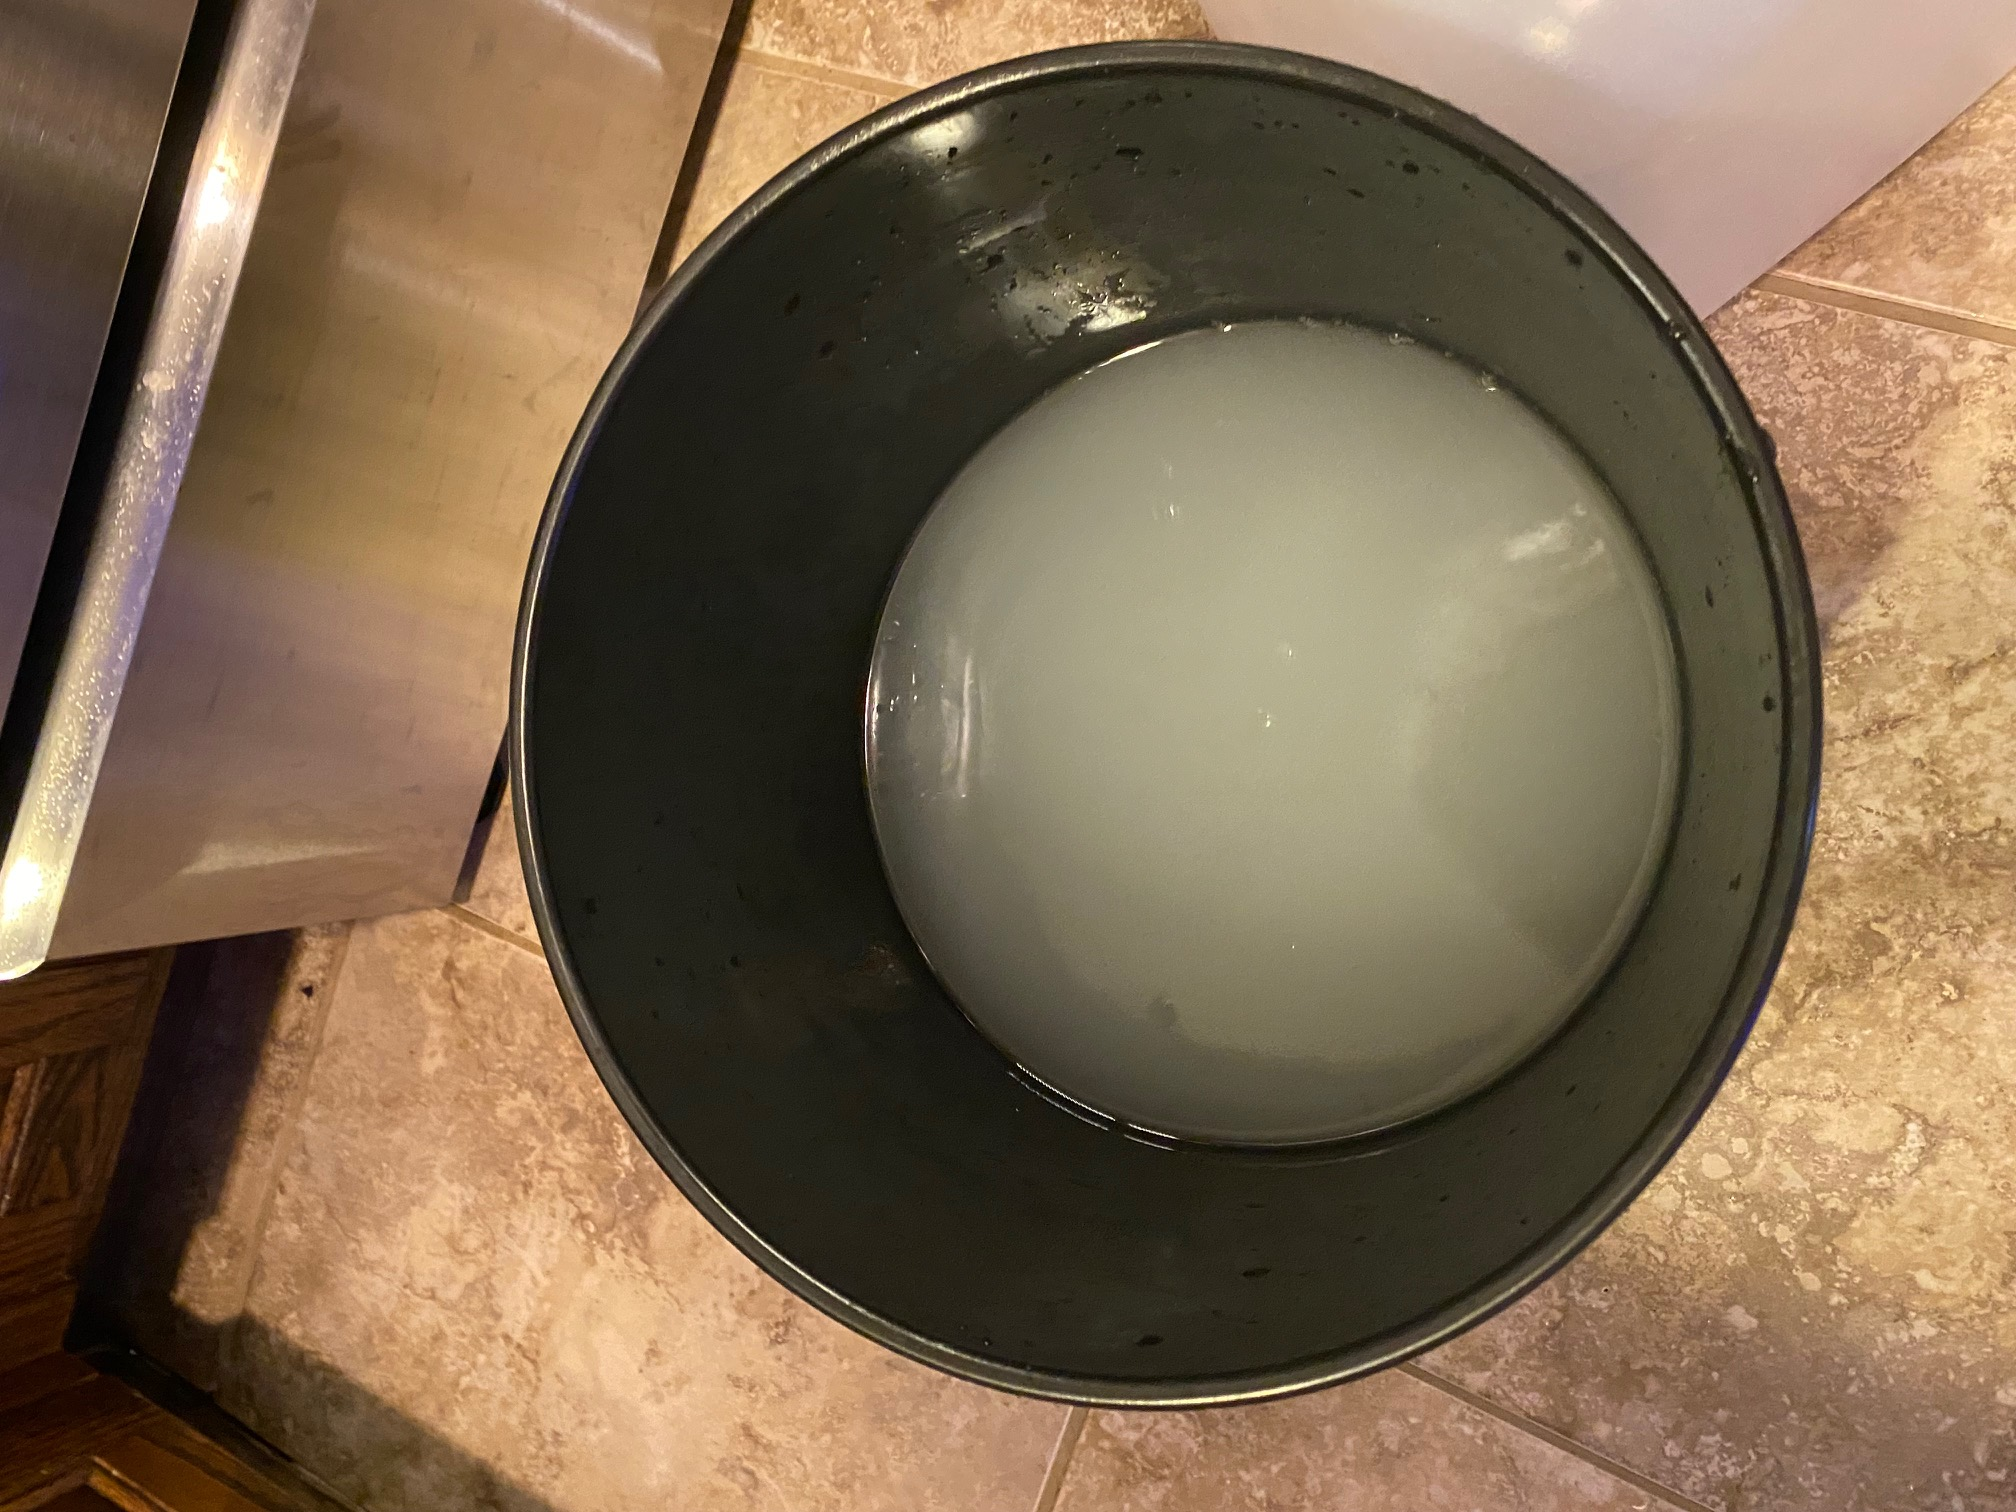
\includegraphics[width=0.9\textwidth, angle=-90]{UnmixedWater.jpg}
            \caption{Undissolved Salt}
        \end{subfigure}%
        \begin{subfigure}{0.5\textwidth}
            \centering
            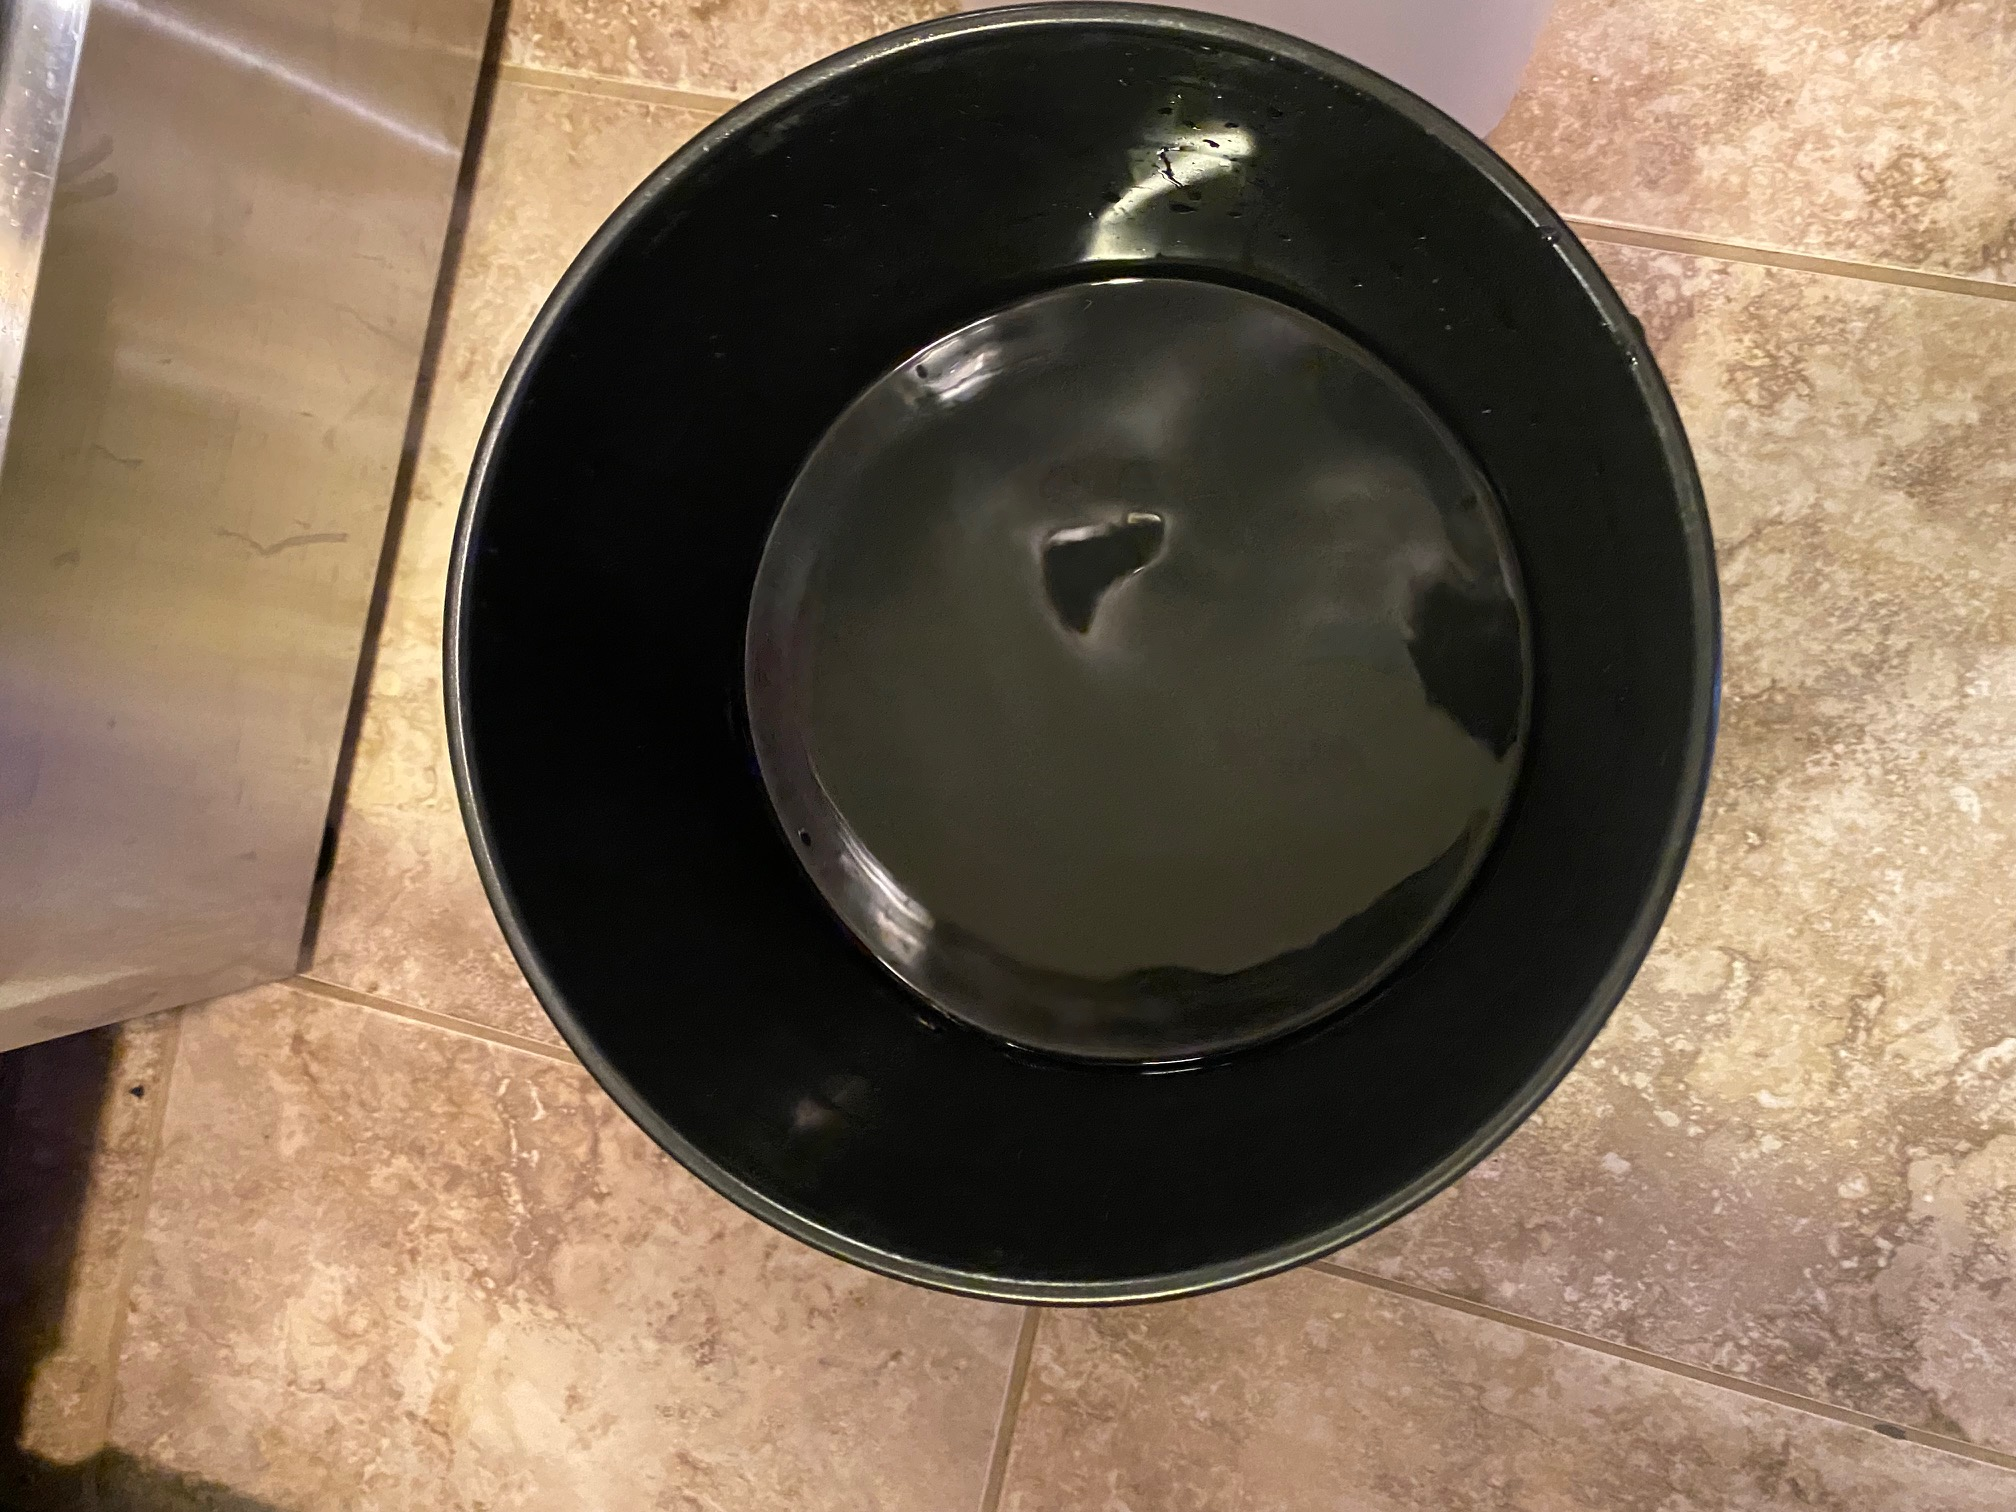
\includegraphics[width=0.9\textwidth, angle=-90]{MixedWater.jpg}
            \caption{Fully Dissolved Salt}
        \end{subfigure}
        \caption{Dissolved and Undissolved Saltwater}
    \end{figure}
    
    \item In the meantime, perform the \hyperref[sec:reefwc]{water change}
    \item Now that the water is clear, we are going to use the refractometer to measure its salinity.
    \begin{enumerate}[I]
    \label{sec:refrinstructions}
        \item Using some RODI water, rinse the pipette that is in the refractometer box.
        \begin{figure}[H]
            \centering
            \begin{subfigure}{0.5\textwidth}
                \centering
                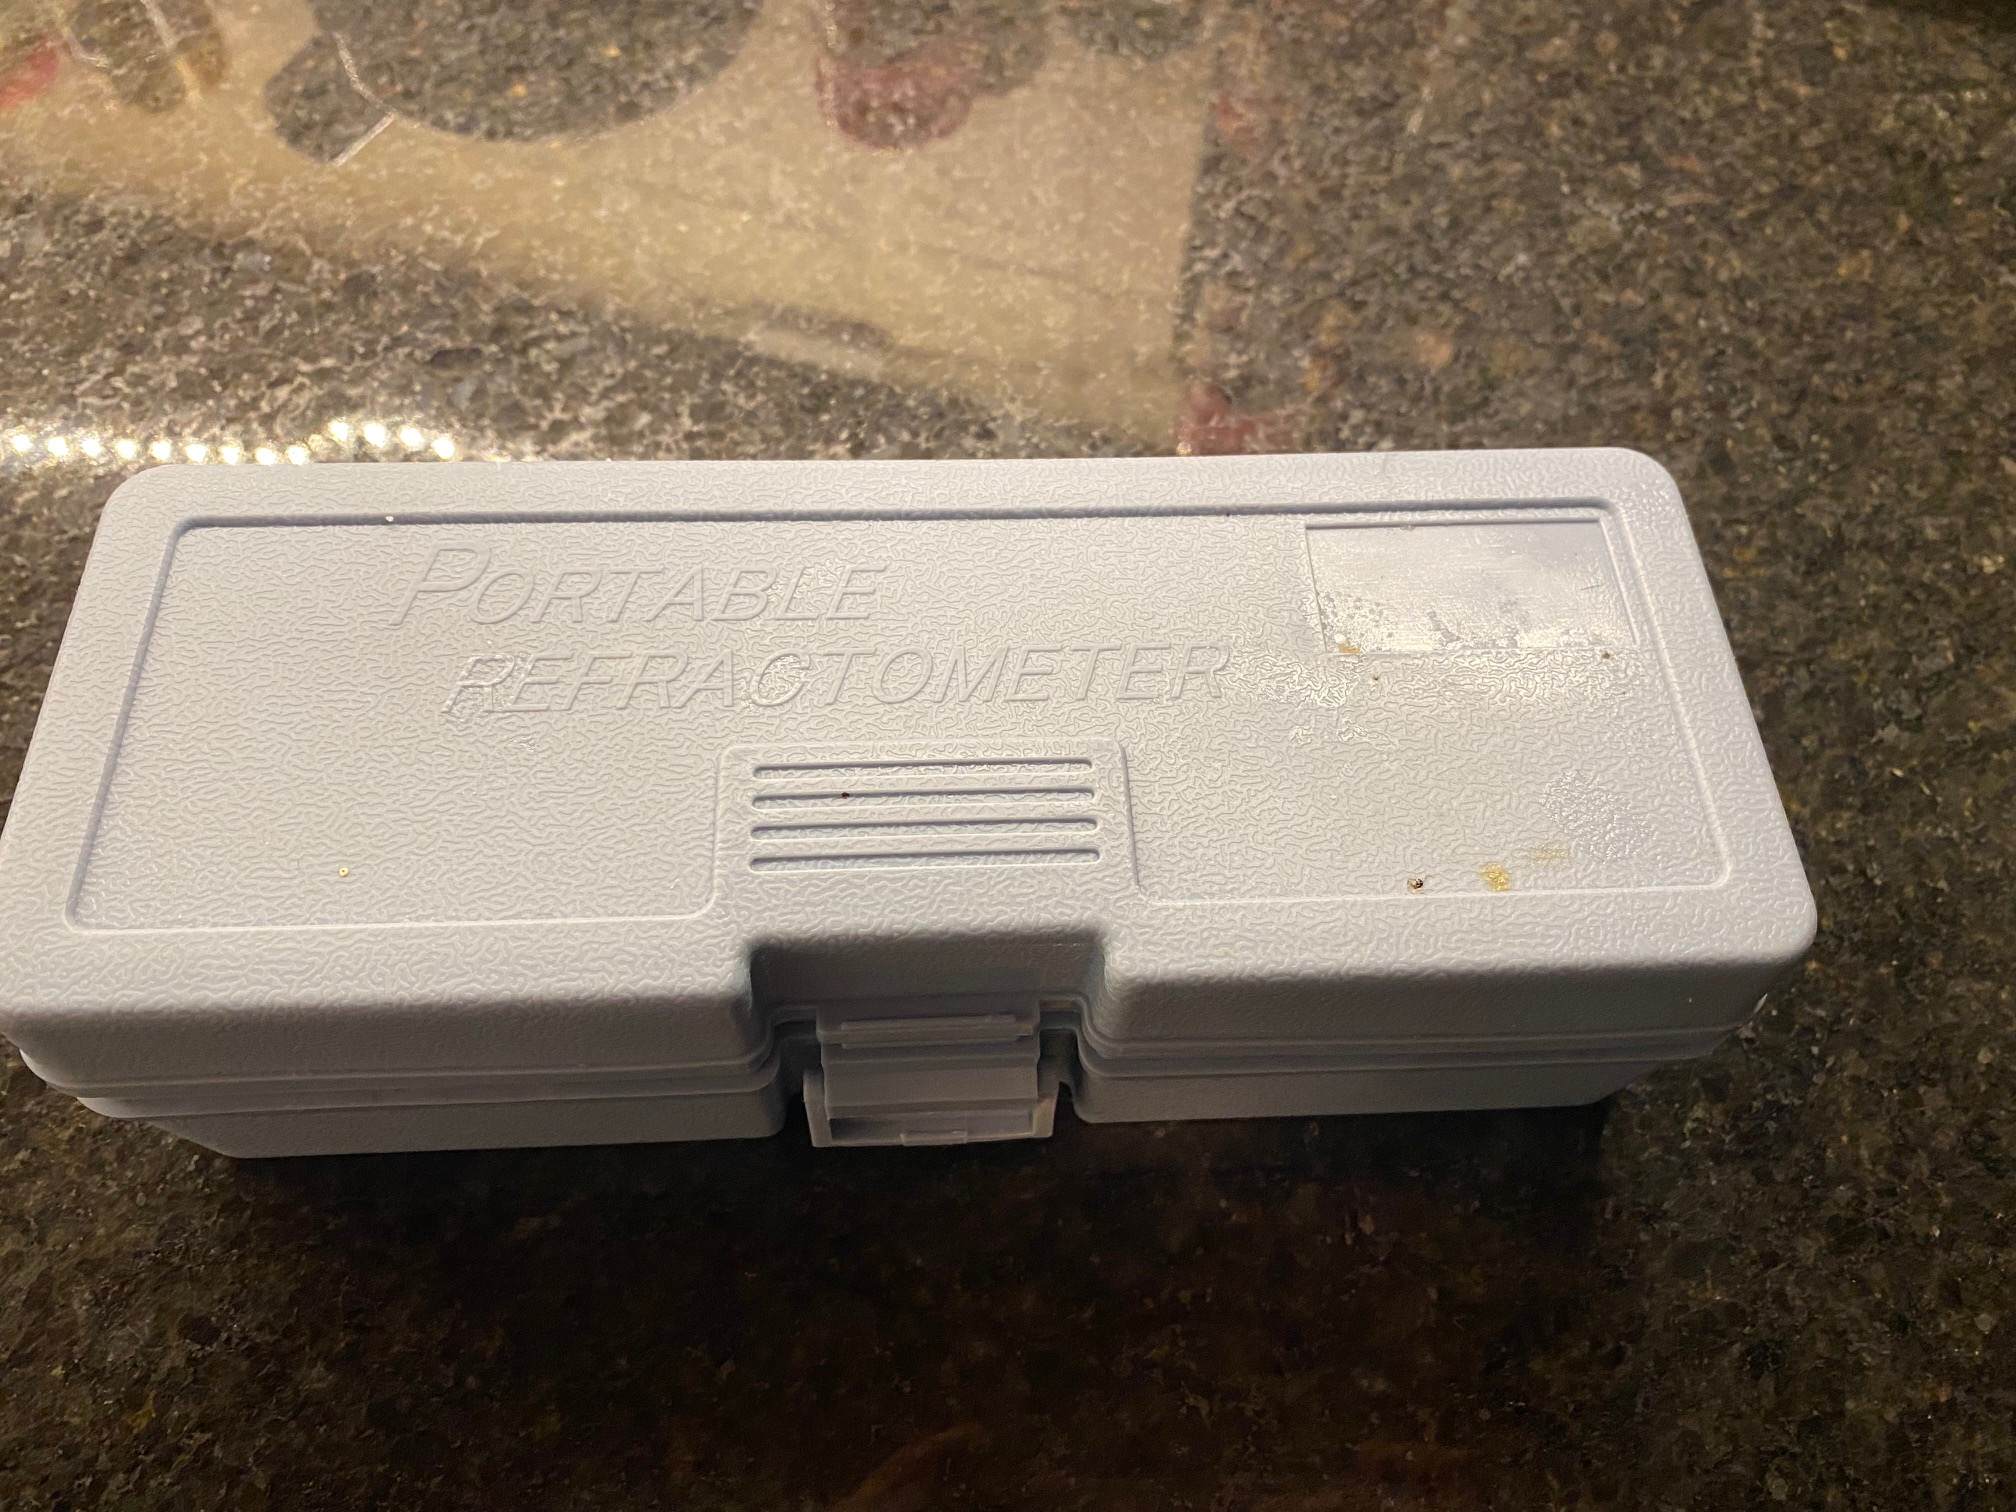
\includegraphics[width=0.9\textwidth]{RefractometerBox.jpg}
                \caption{The refractometer box}
            \end{subfigure}%
            \begin{subfigure}{0.5\textwidth}
                \centering
                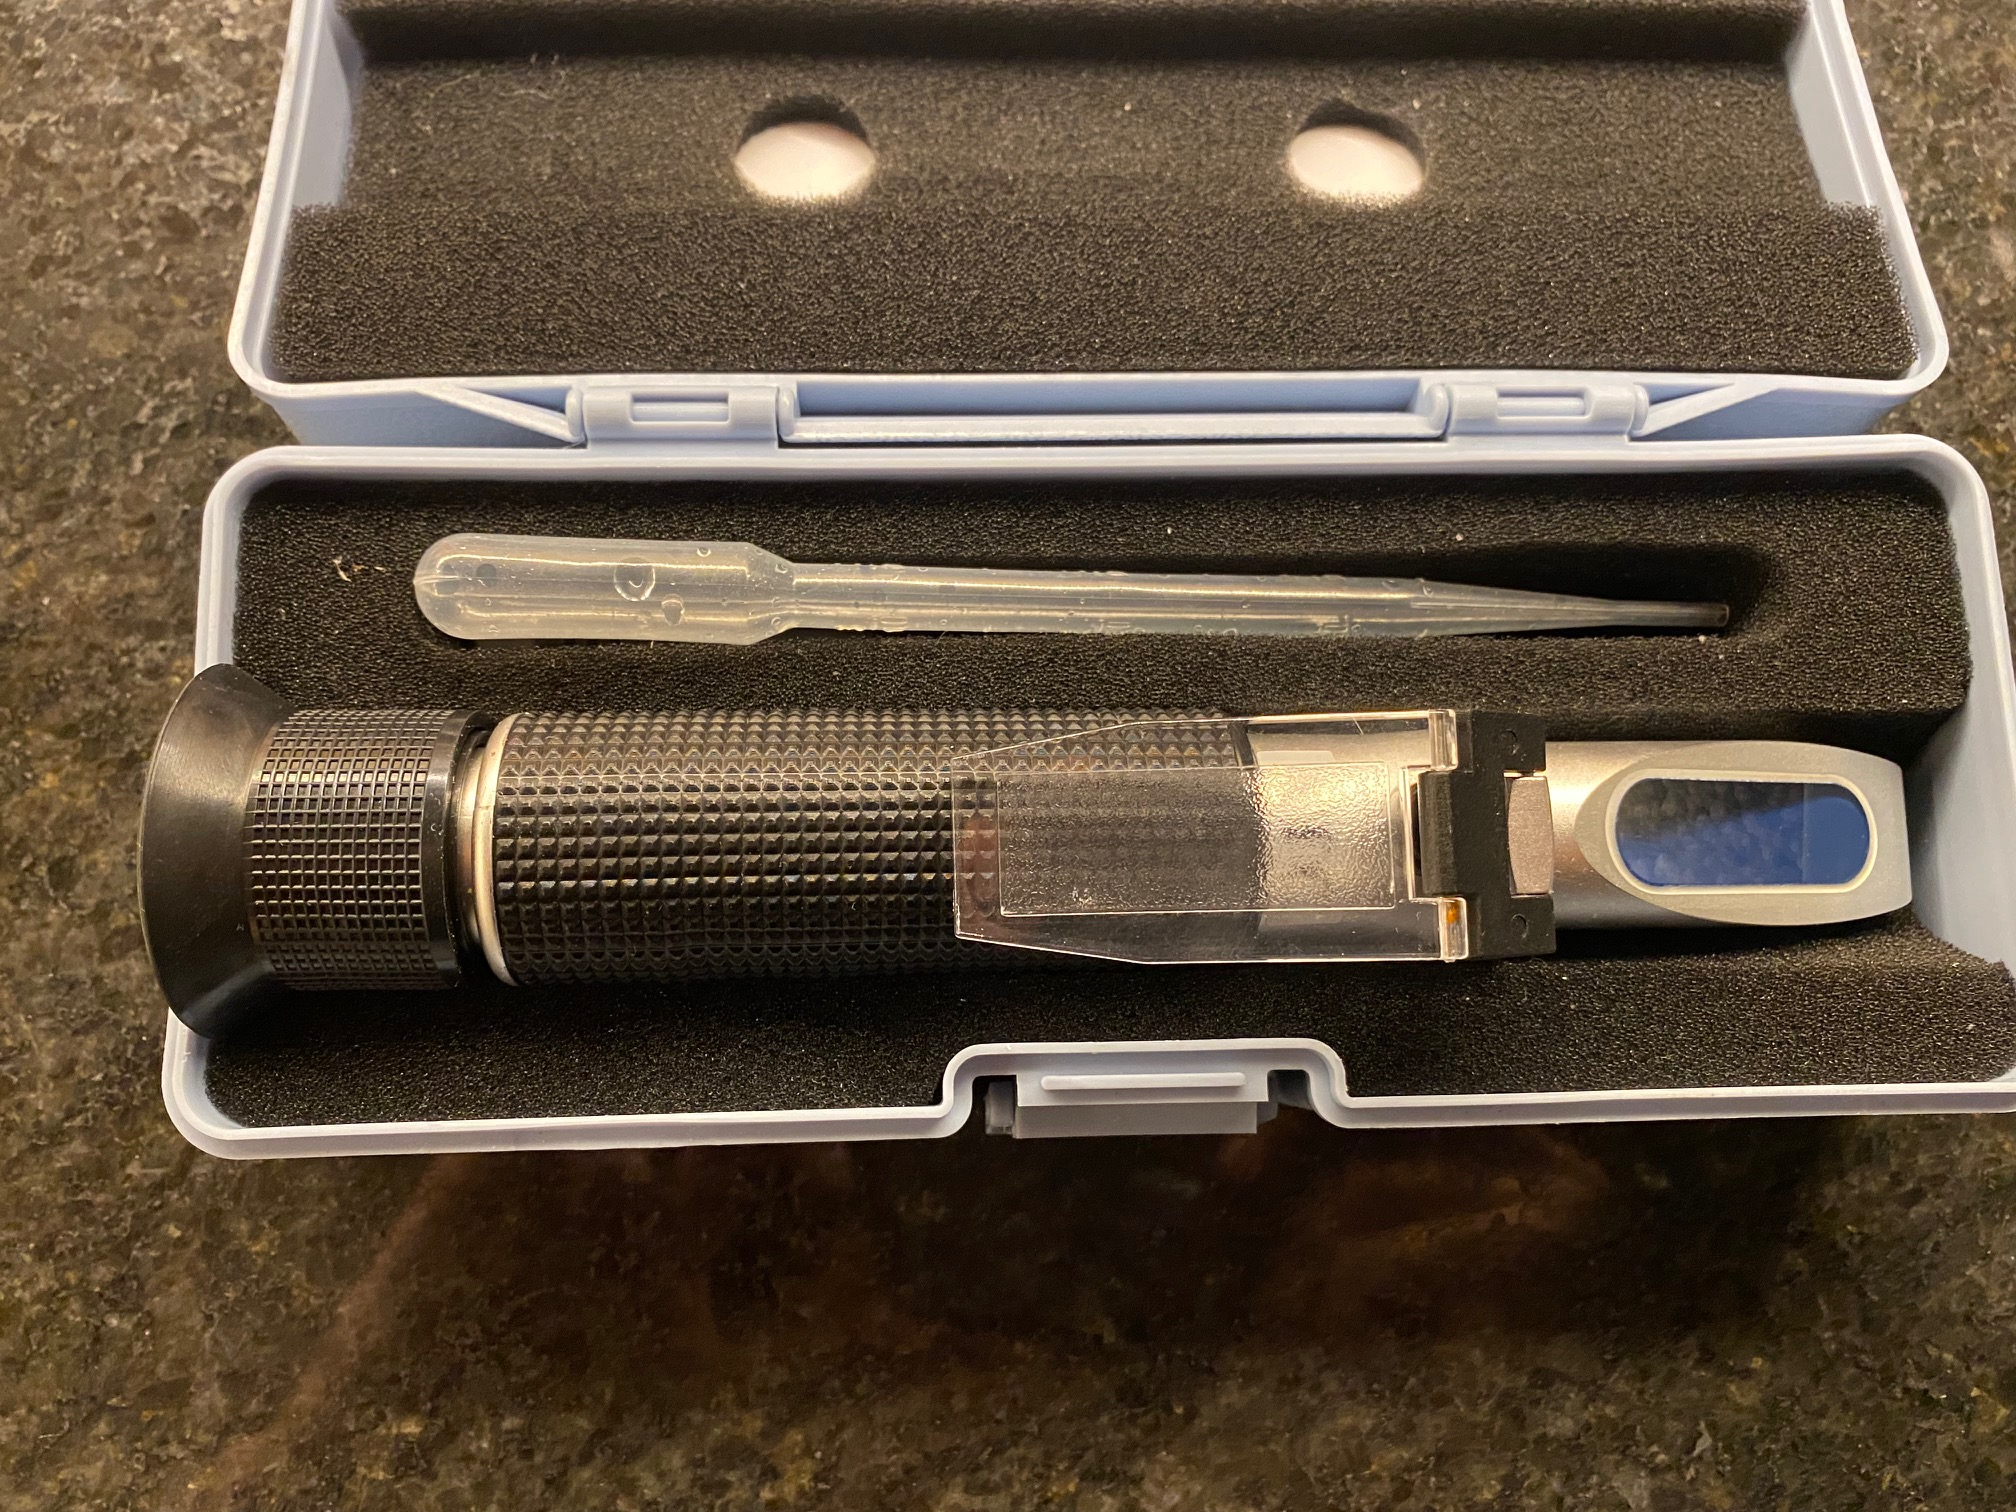
\includegraphics[width=0.9\textwidth]{RefractometerInBox.jpg}
                \caption{Contents of the refractometer box}
            \end{subfigure}
            \caption{Refractometer}
        \end{figure}
        
        \item Squirt some RODI water onto the refractometer sample glass. Use a paper towel to throroughly clean the glass.
        \item Repeat step II.
        \item Empty the pipette of any RODI water in it. 
        \item Rinse the pipette with water from the aquarium. Flush it multiple times.
        \item Use the pipette to put a large bead of water on the exposed glass of the refractometer. Close the plastic lid 
        on top. This will splash water a little bit. 
        \begin{figure}[H]
            \centering
            \begin{subfigure}{0.5\textwidth}
                \centering
                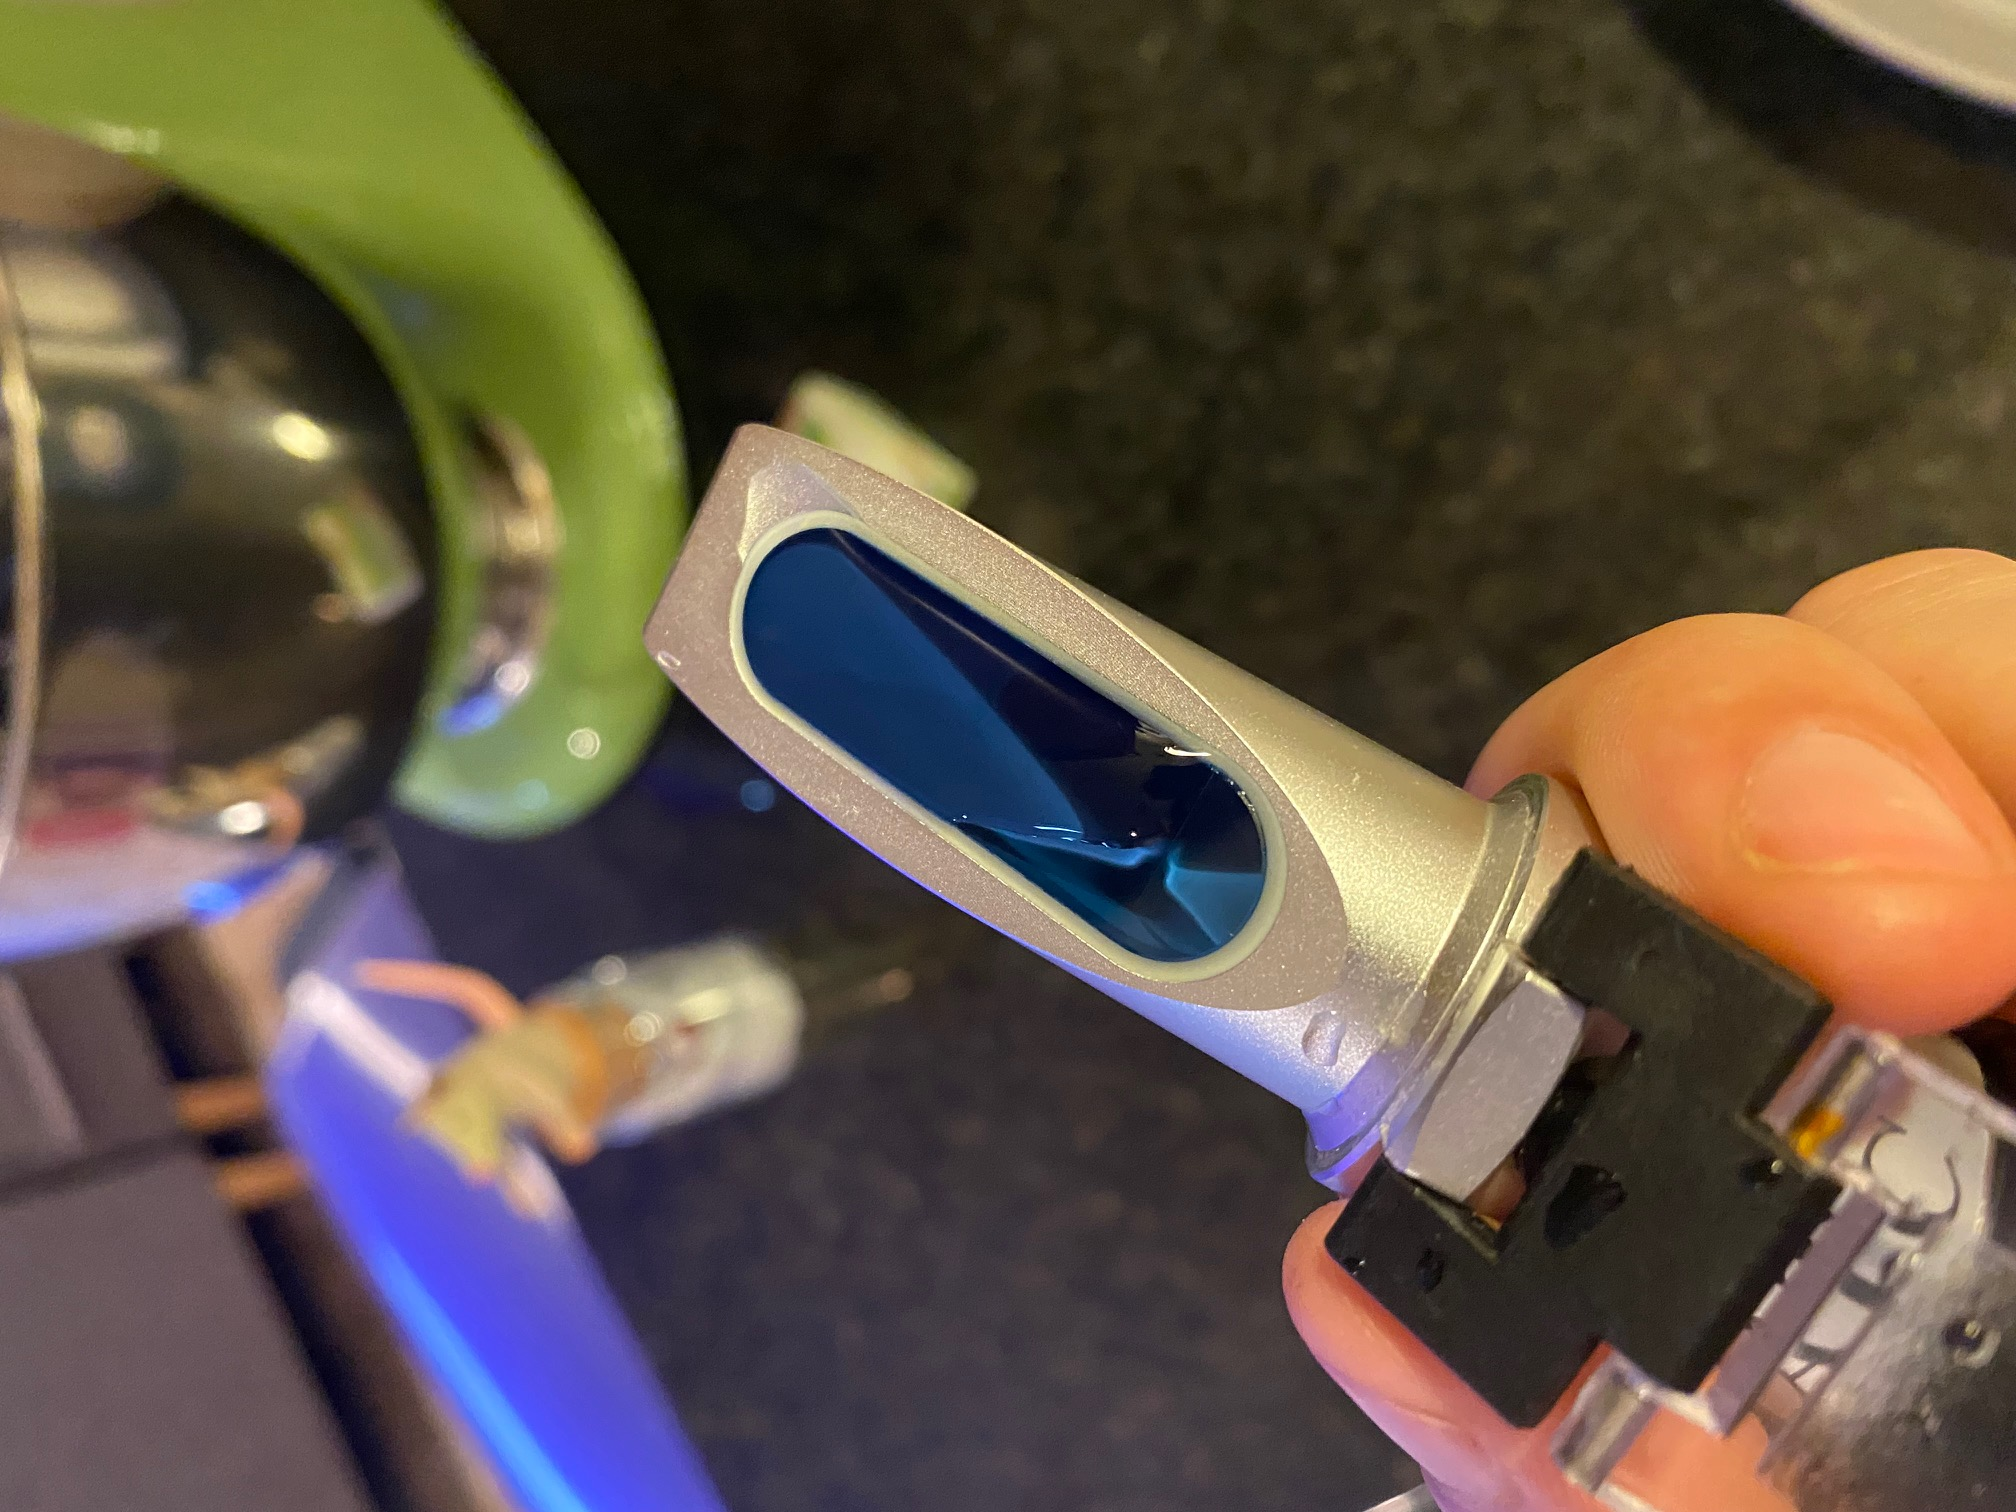
\includegraphics[width=0.9\textwidth, angle=-90]{OpenRefractometer.jpg}
                \caption{A bead of water on the sample glass}
            \end{subfigure}%
            \begin{subfigure}{0.5\textwidth}
                \centering
                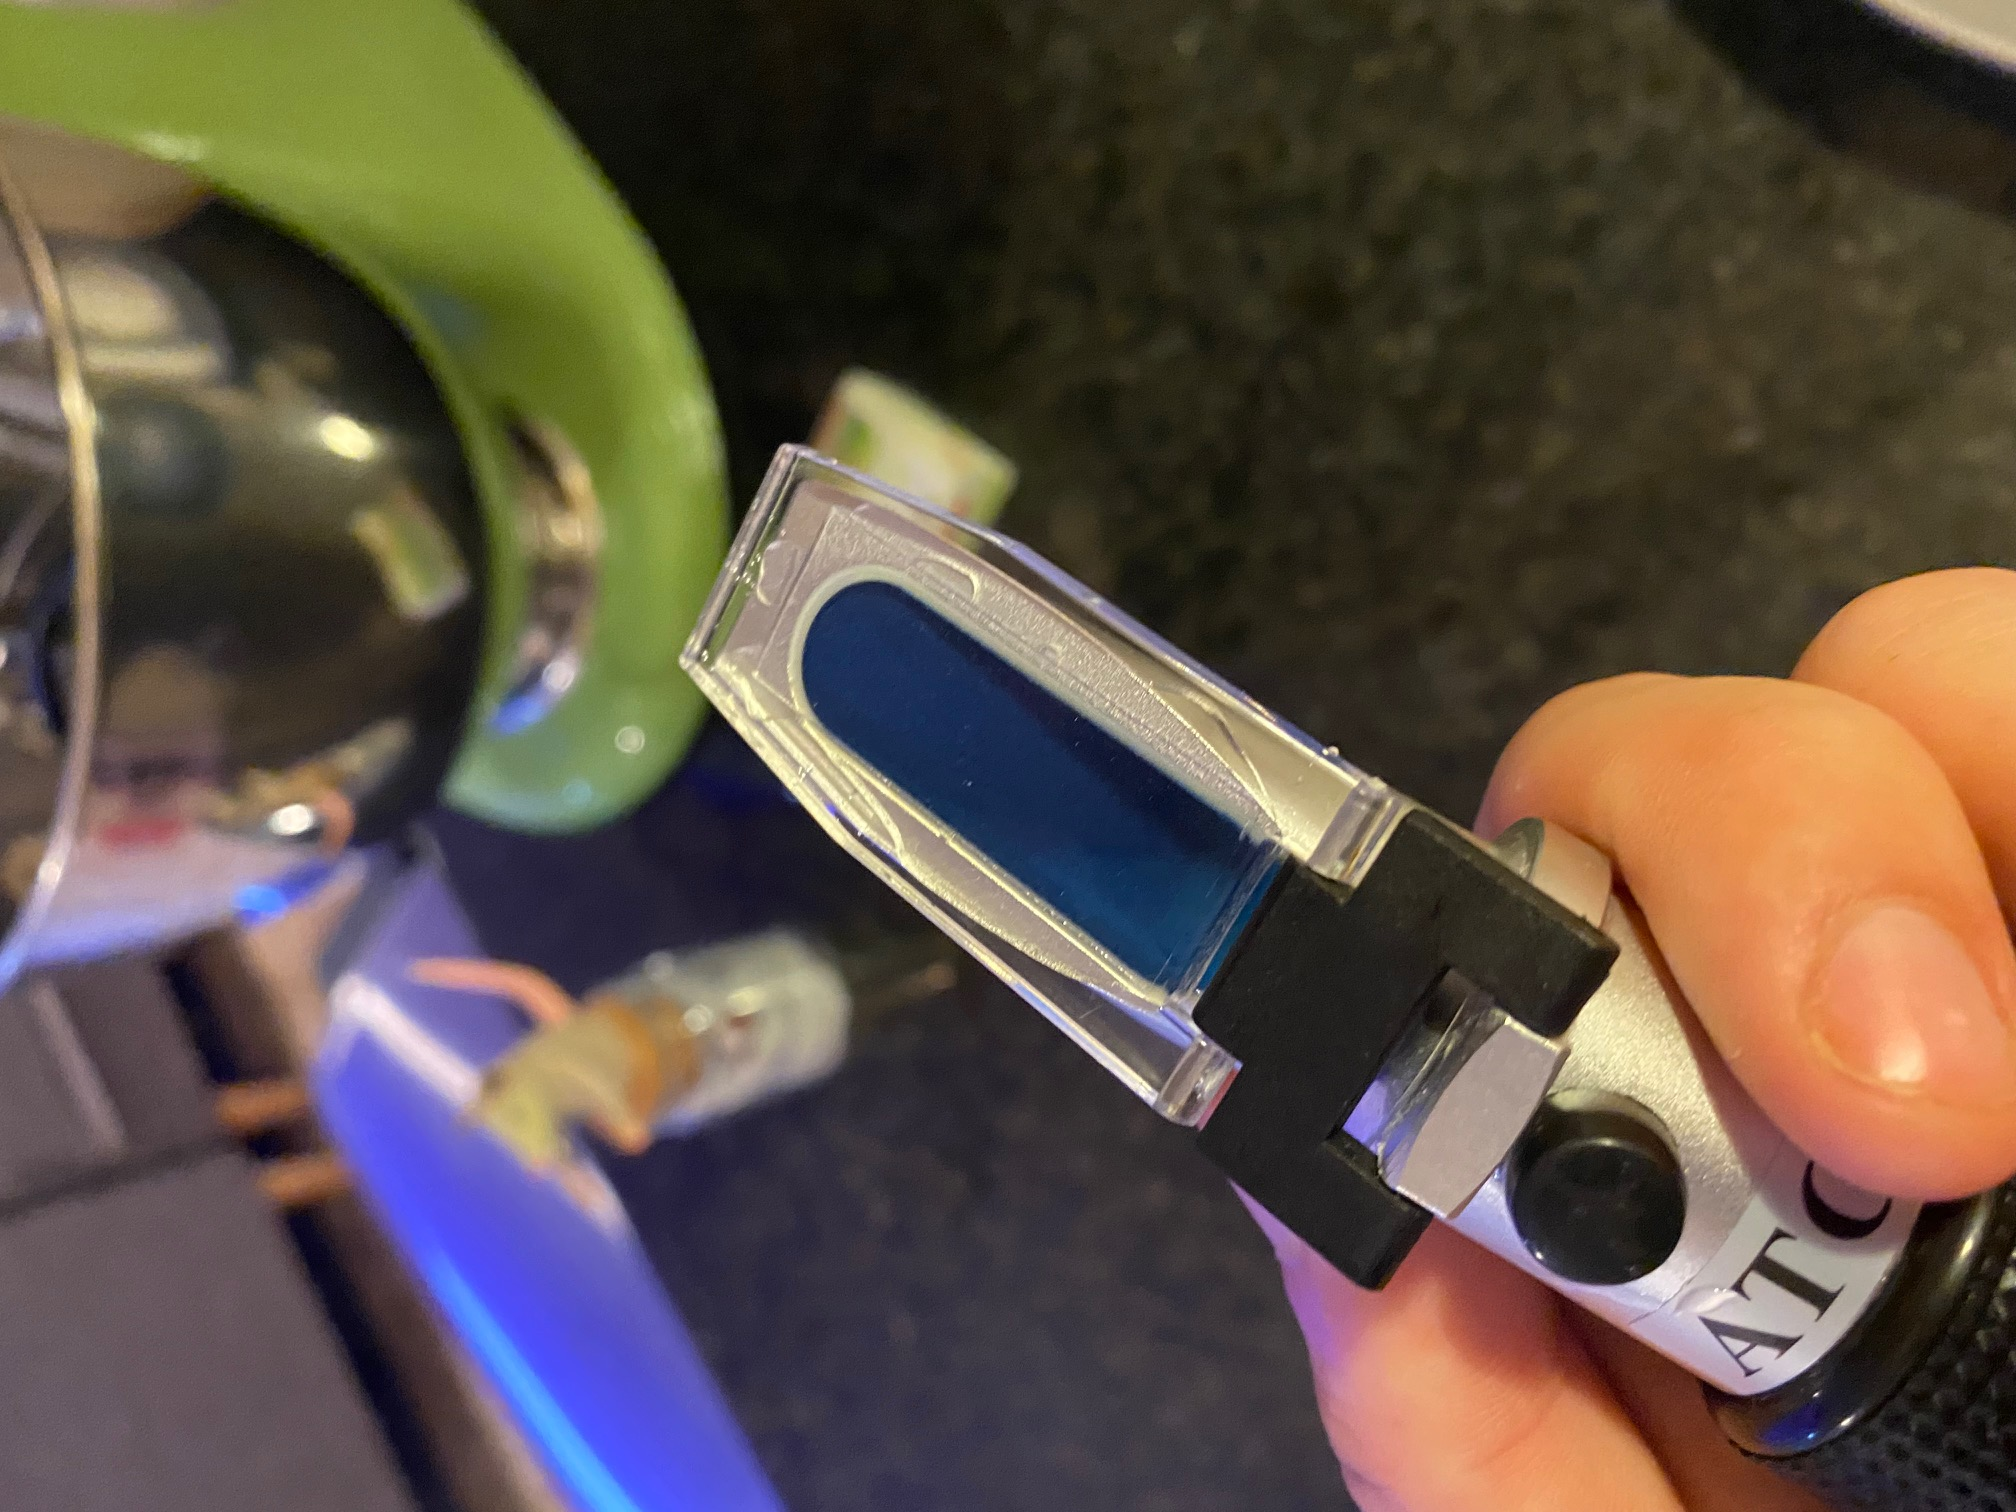
\includegraphics[width=0.9\textwidth, angle=-90]{ClosedRefractometer.jpg}
                \caption{The closed refractometer}
            \end{subfigure}
            \caption{Refractometer Operation}
        \end{figure}
        
        \item Hold the refractometer up to a warm light source. Sunlight works best, but incandescent bulbs work too. LEDs 
        tend not to work very well. Look into the eyepiece. You may have to move around to find the right viewing angle. The eyepiece is 
        adjustable to focus the picture. 
        \begin{figure}[H]
            \centering
            \begin{subfigure}{0.5\textwidth}
                \centering
                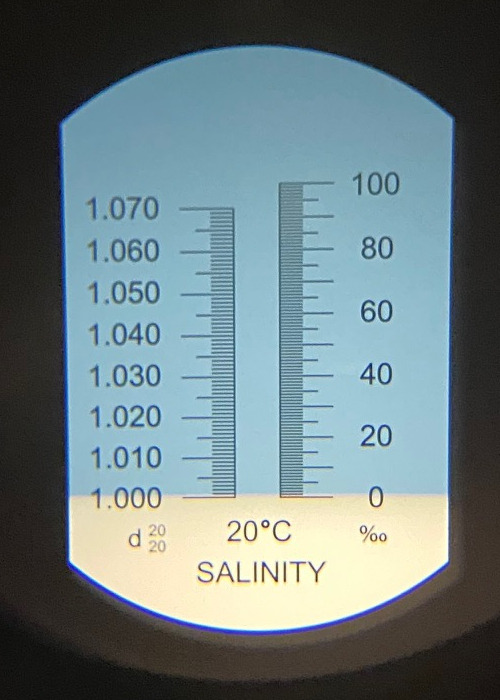
\includegraphics[width=0.9\textwidth]{RefractometerReading.jpg}
                \caption{A reading of 0 ppt.}
            \end{subfigure}%
            \begin{subfigure}{0.5\textwidth}
                \centering
                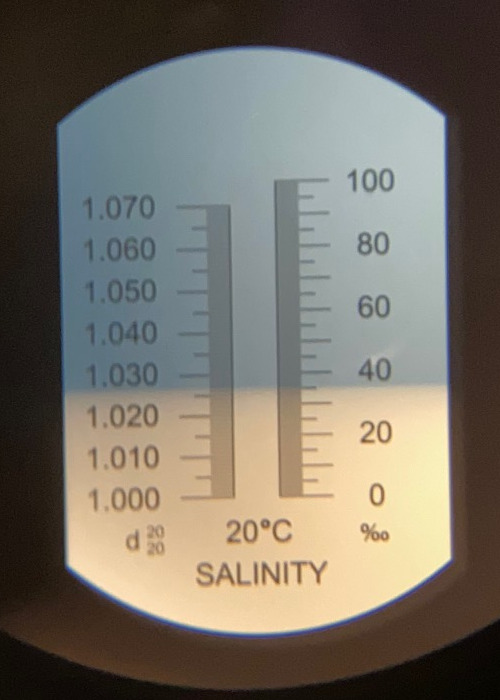
\includegraphics[width=0.9\textwidth]{Salinity.jpg}
                \caption{A reading of 35 ppt.}
            \end{subfigure}
            \caption{Refractometer Readings}
        \end{figure}
        
        \item Look for where the dark line ends on the scale. This reading is the salinity of the water.
        \item Repeat these steps 2-3 times, or until you get three nearly identical readings.
        \item Repeat the steps all over, but for the newly "brewed" saltwater. 
        \item Verify that the saltwater's salinity is equal to or slightly above that of the aquarium.
    \end{enumerate}

    \item Congratulations! You're done preparing the water!
\end{enumerate}

\subsection{Water Changes}
\label{sec:reefwc}
Actually performing the water change is pretty easy. Lucky you!
\begin{enumerate}
    \item Unplug the pumps and remove the glass topcover.
    \item Remove the auto top-off bottle.
    \item Using the same hose as was used for the freshwater aquarium's water change, put on end of the hose into the 
    5-gallon jug with liter markings on it.
    \item Hold the other end of the hose in the reef tank's water.
    \item Start a siphon by sucking lightly on the waste end of the tube.
    \begin{figure}[H]
        \centering
        \begin{subfigure}{0.5\textwidth}
            \centering
            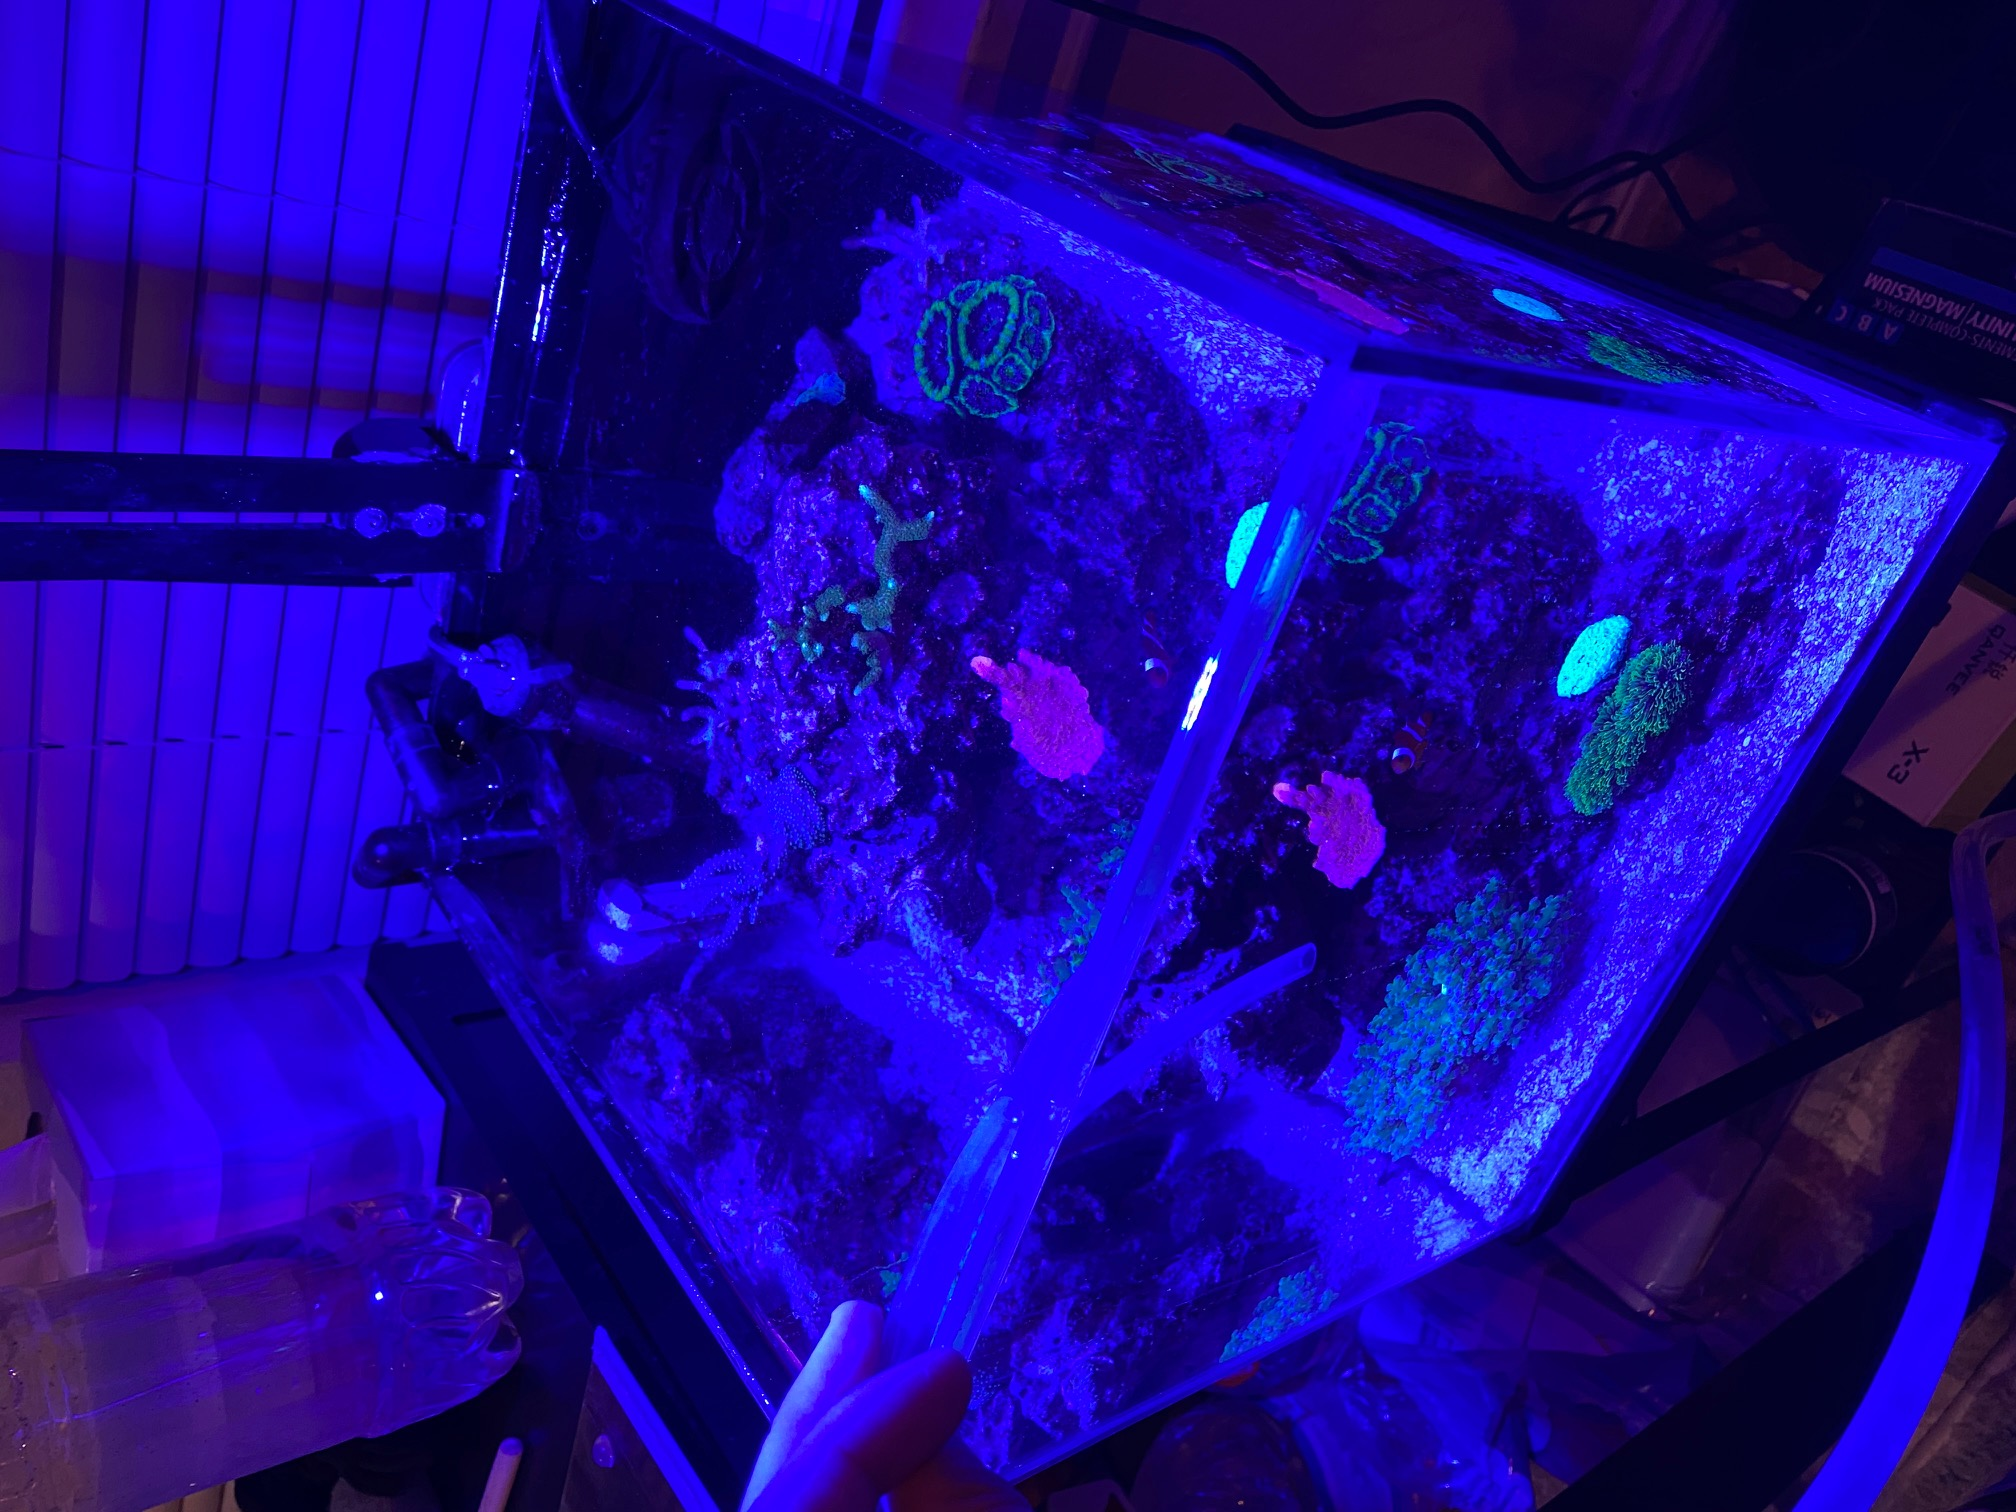
\includegraphics[width=0.9\textwidth, angle=-90]{EmptyingAquarium.jpg}
            \caption{Siphoning water from the tank}
        \end{subfigure}%
        \begin{subfigure}{0.5\textwidth}
            \centering
            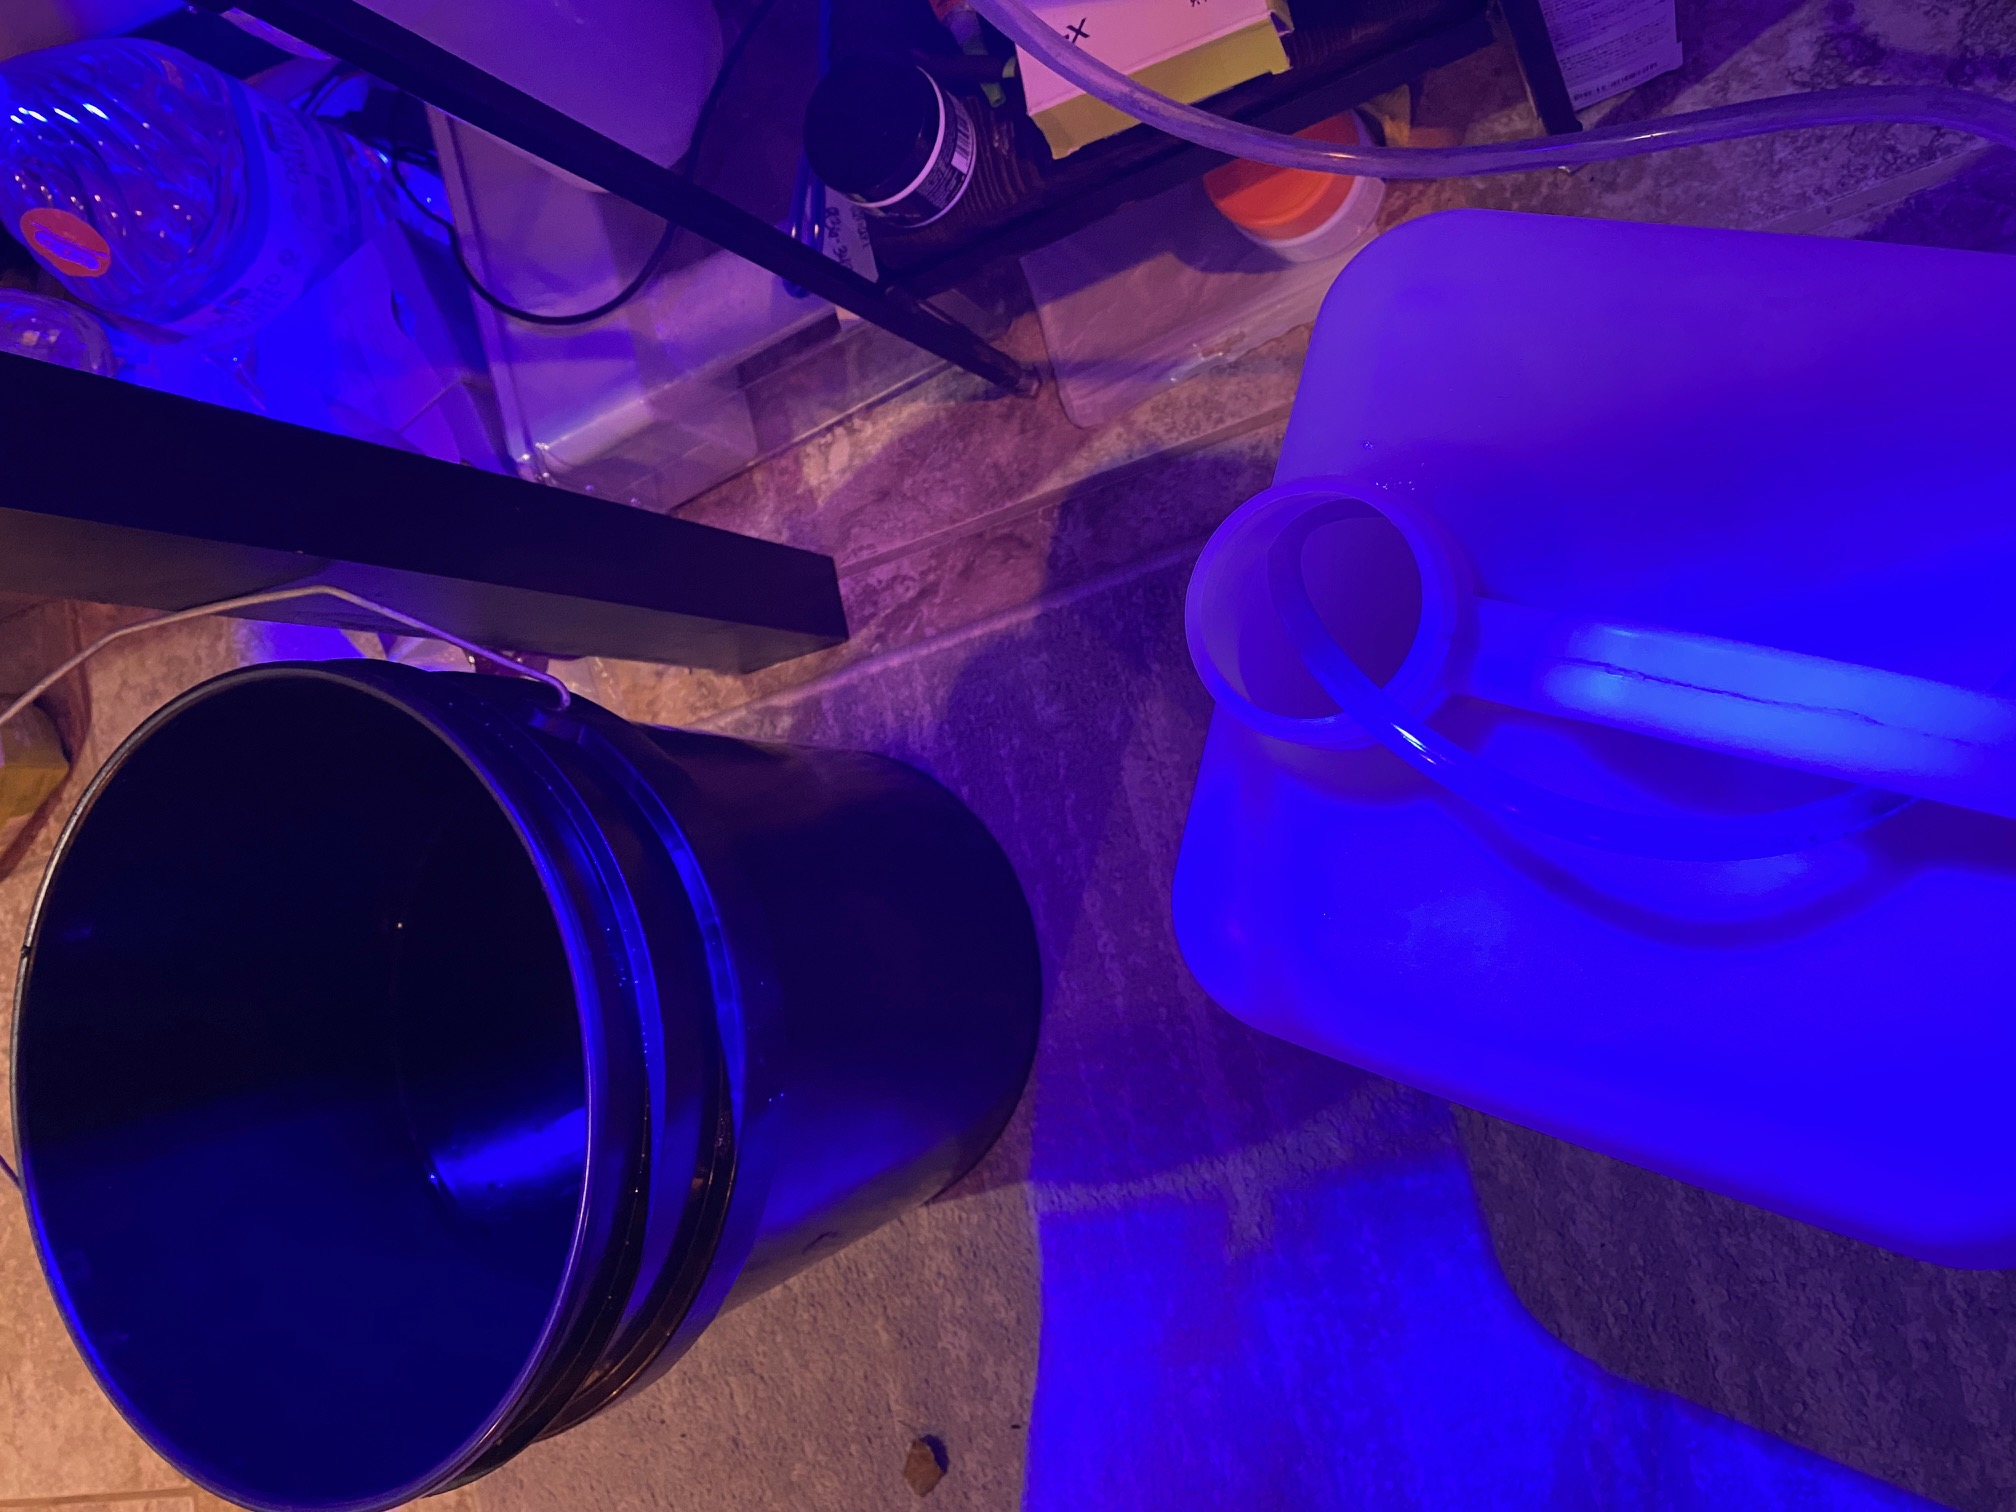
\includegraphics[width=0.9\textwidth, angle=-90]{WasteJug.jpg}
            \caption{Water flowing into the waste jug}
        \end{subfigure}
        \caption{Emptying the reef tank}
    \end{figure}
    
    \item drain not more than 8 liters of water from the tank. 
    \item Do not dump the water yet.
    \item Carefully refill the aquarium using the water you prepared in \hyperref[sec:waterprep]{ the previous section}. Fill 
    the tank up to the line on the light mount. 
    \begin{figure}[H]
        \centering
        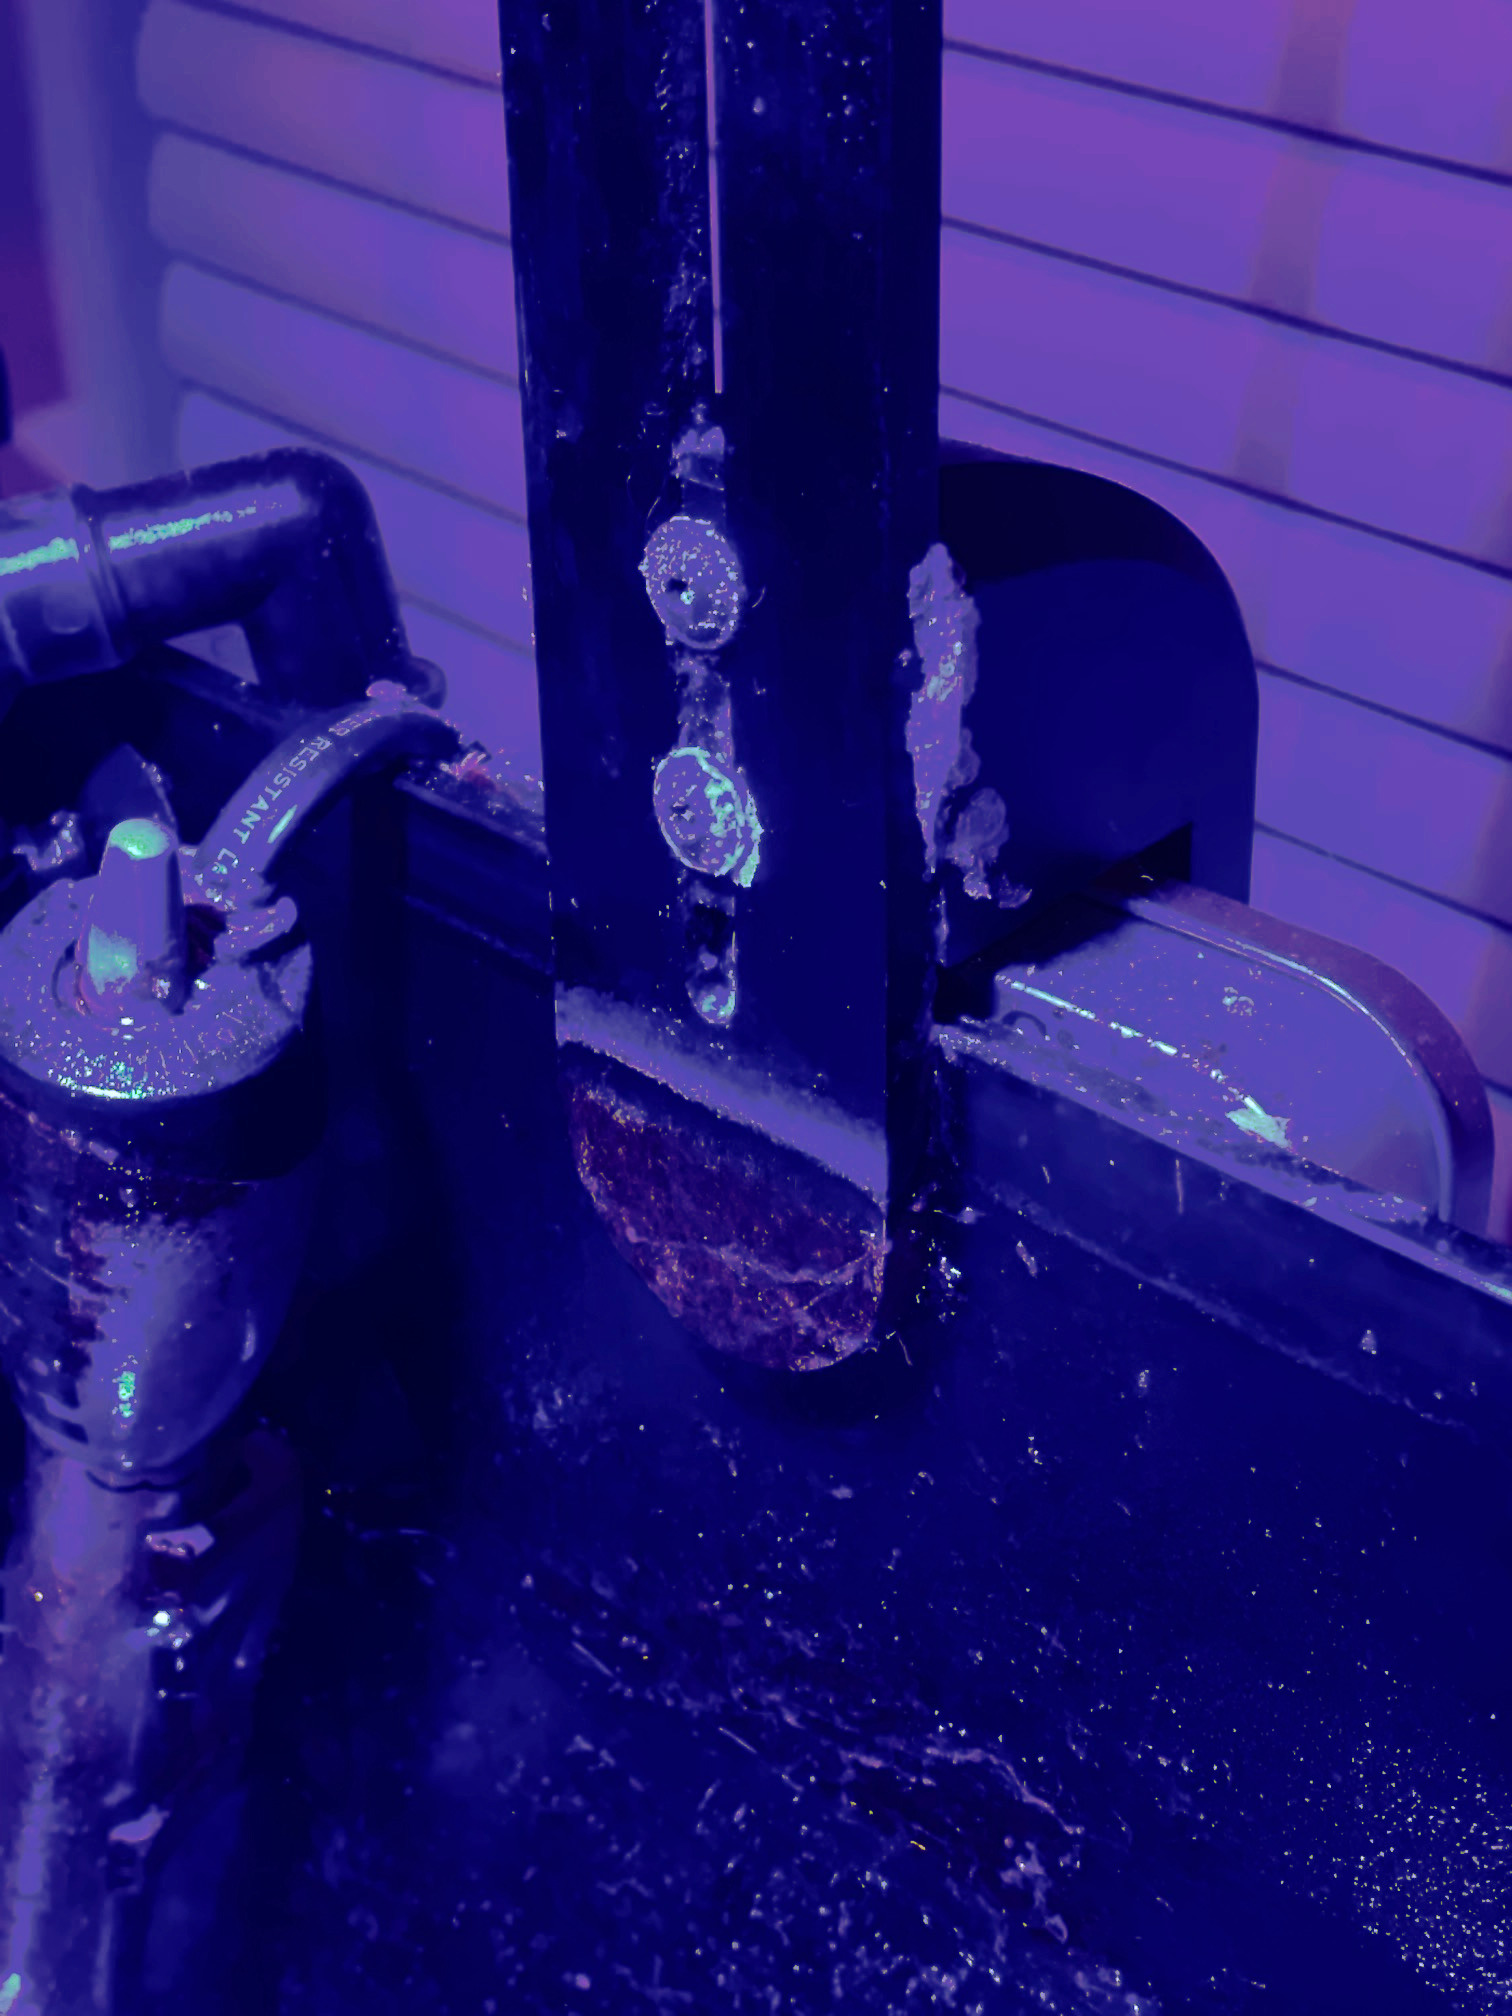
\includegraphics[width=0.5\textwidth]{WaterLine.jpg}
        \caption{The water line on the light mount}
    \end{figure}
    
    \item If there is not enough water to fill the tank to the line, add some old tankwater back in. 
    \item Plug the pumps back in, put the auto-top-off bottle back on the tank, and replace the glass cover.
    \item Dump any leftover saltwater and all the wastewater.
\end{enumerate}

\subsection{Filter Maintenance}
Filter maintenance is hell. Please don't touch it. 

\subsection{Algae Maintenance}
\label{sec:algaescraper}
Algae naturally grows on the glass of the aquarium. This isn't harmful to the tank, but it is quite ugly. Cleaning it off is simple and quick. 

The algae scraper is in a long flat box underneath the aquarium stand. Assemble the tool using the long metal rod, the knurled handle, and the blade component. Keep the blade's sheath on it until you are ready to use it.

Remove the glass lid of the aquarium. Don't turn off the circulation pump. 

Remove the sheath of the blade. Notice that the blade is at an angle compared to the shaft of the scraper. You want the blade to be at 
around an 45$^{\circ}$ angle with the glass. 

\begin{figure}[H]
    \centering
    \begin{subfigure}{0.5\textwidth}
        \centering
        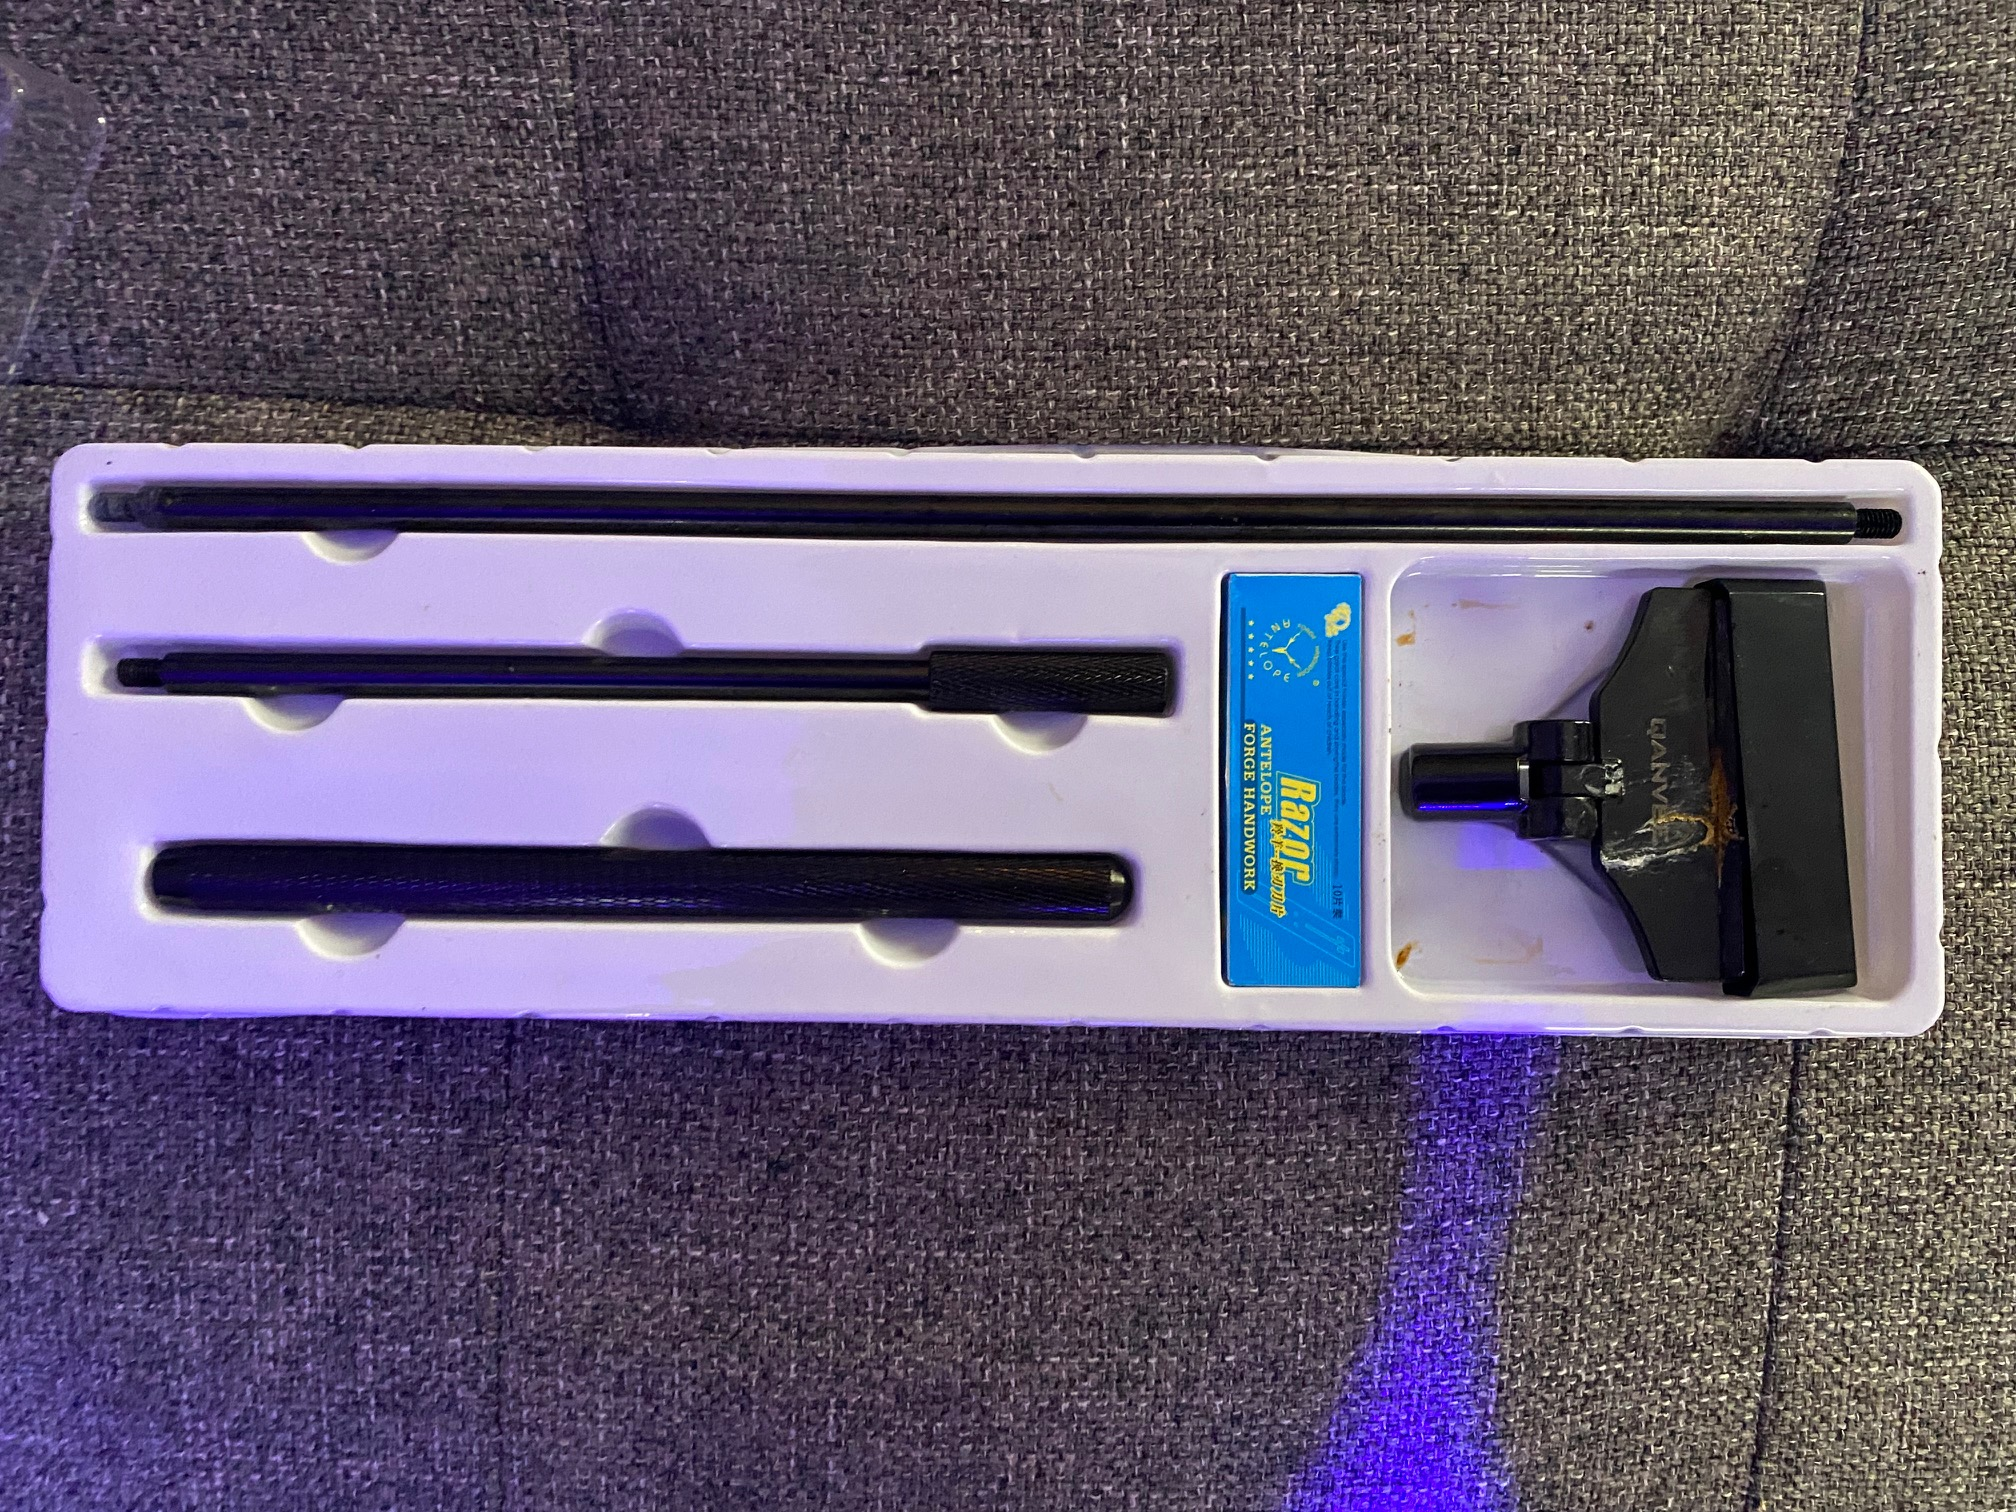
\includegraphics[width=0.9\textwidth]{ScraperBox.jpg}
        \caption{Algae Scraper In Box}
    \end{subfigure}%
    \begin{subfigure}{0.5\textwidth}
        \centering
        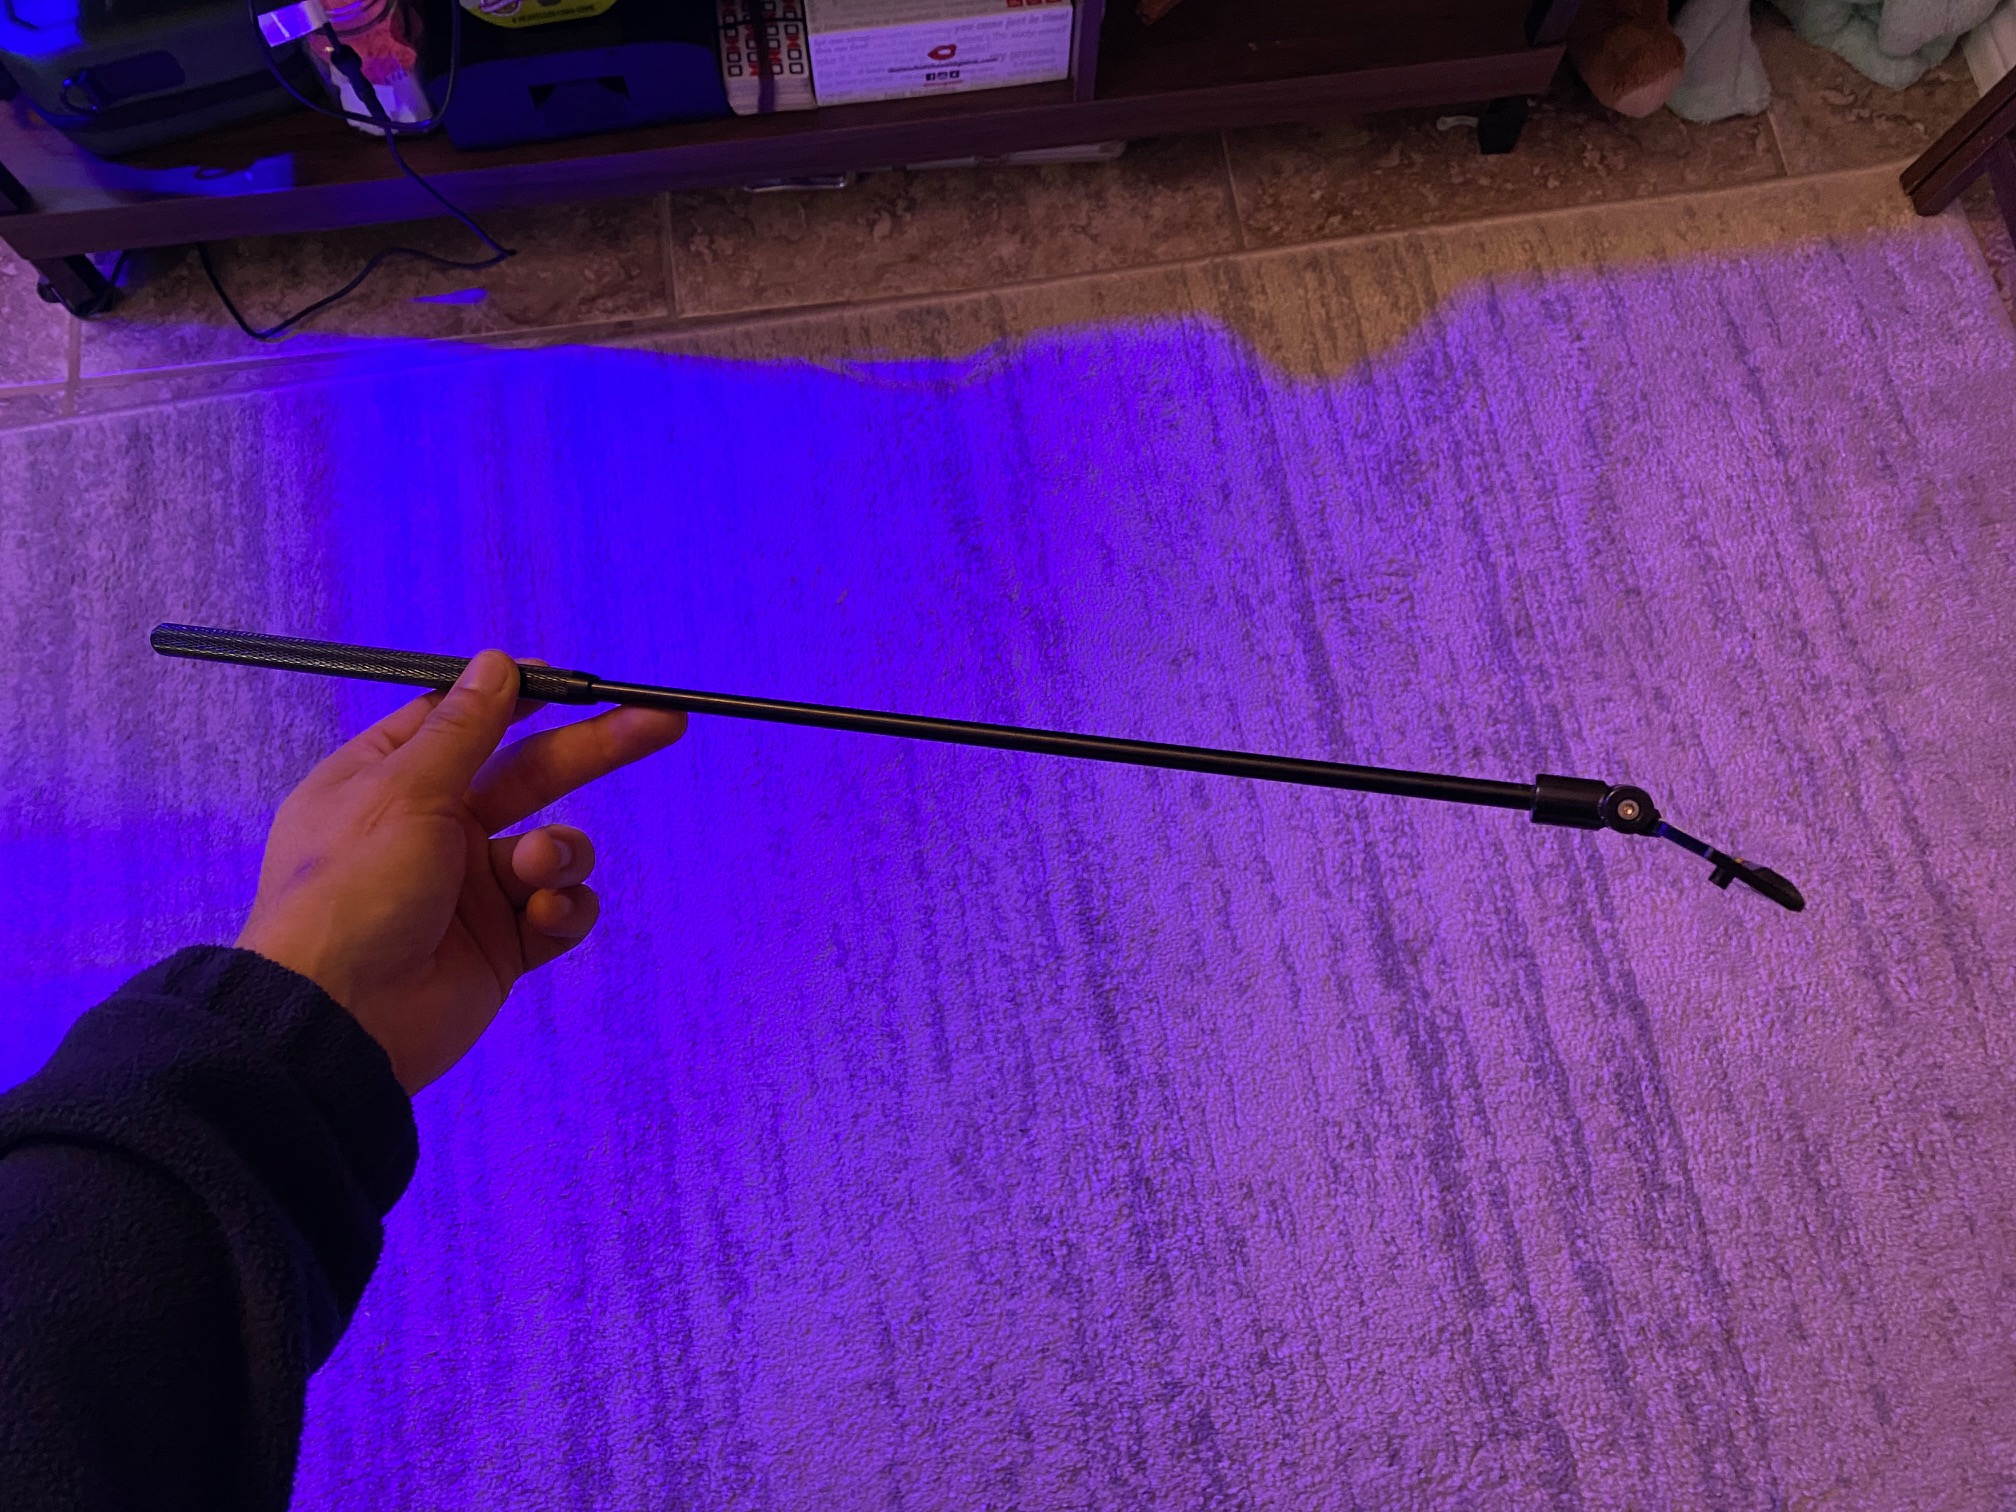
\includegraphics[width=0.9\textwidth]{Scraper.jpg}
        \caption{Algae Scraper Assembled}
    \end{subfigure}
    \caption{The Algae Scraper}
\end{figure}

Dip the scraper blade into the aquarium, at around a 45$^{\circ}$ angle with the glass and press firmly. Go down the height 
of the glass in one straight line, then come back up in the same line, while continuing to apply pressure. Move the scraper 
by around half of it's width and repeat the same procedure. You want around a 50\% overlap between each pass. The corners of 
the tank will require multiple passes. Around the left side of the tank, there are some corals and rocks that stick out a 
bit. Be careful around them and avoid hitting them. If you don't think you can avoid them, just don't scrape that area -- it 
really doesn't matter.

\section{Lighting}
Unlike the freshwater aquarium, the reef tank's light is WiFi-capable and will set itself properly in case of a power outage. 
No maintenance or work should be required for the light. However, please notify me if the color suddenly changes or if it 
seems like the light's fan is constantly on. There is an app that controls the light, but the light's schedule and 
intensities shouldn't be messed around with. 

\newpage
\chapter{Conclusion}
Thank you for taking care of my babies! I really appreciate the help. I hope they bring to you some of the joy they bring to me. As a final note, I would like to say that mistakes happen (I should know, I make a lot of them). It would be highly unlikely for anything bad to happened to the freshwater tank, but unfortunately, saltwater tanks are much more finicky. If any corals die during the break (especially the \textit{Acropora}, \textit{Alveopora}, or the birdsnest) it's completely fine. Shit happens. Just let me know so I can provide further guidance.

\begin{figure}[H]
    \centering
    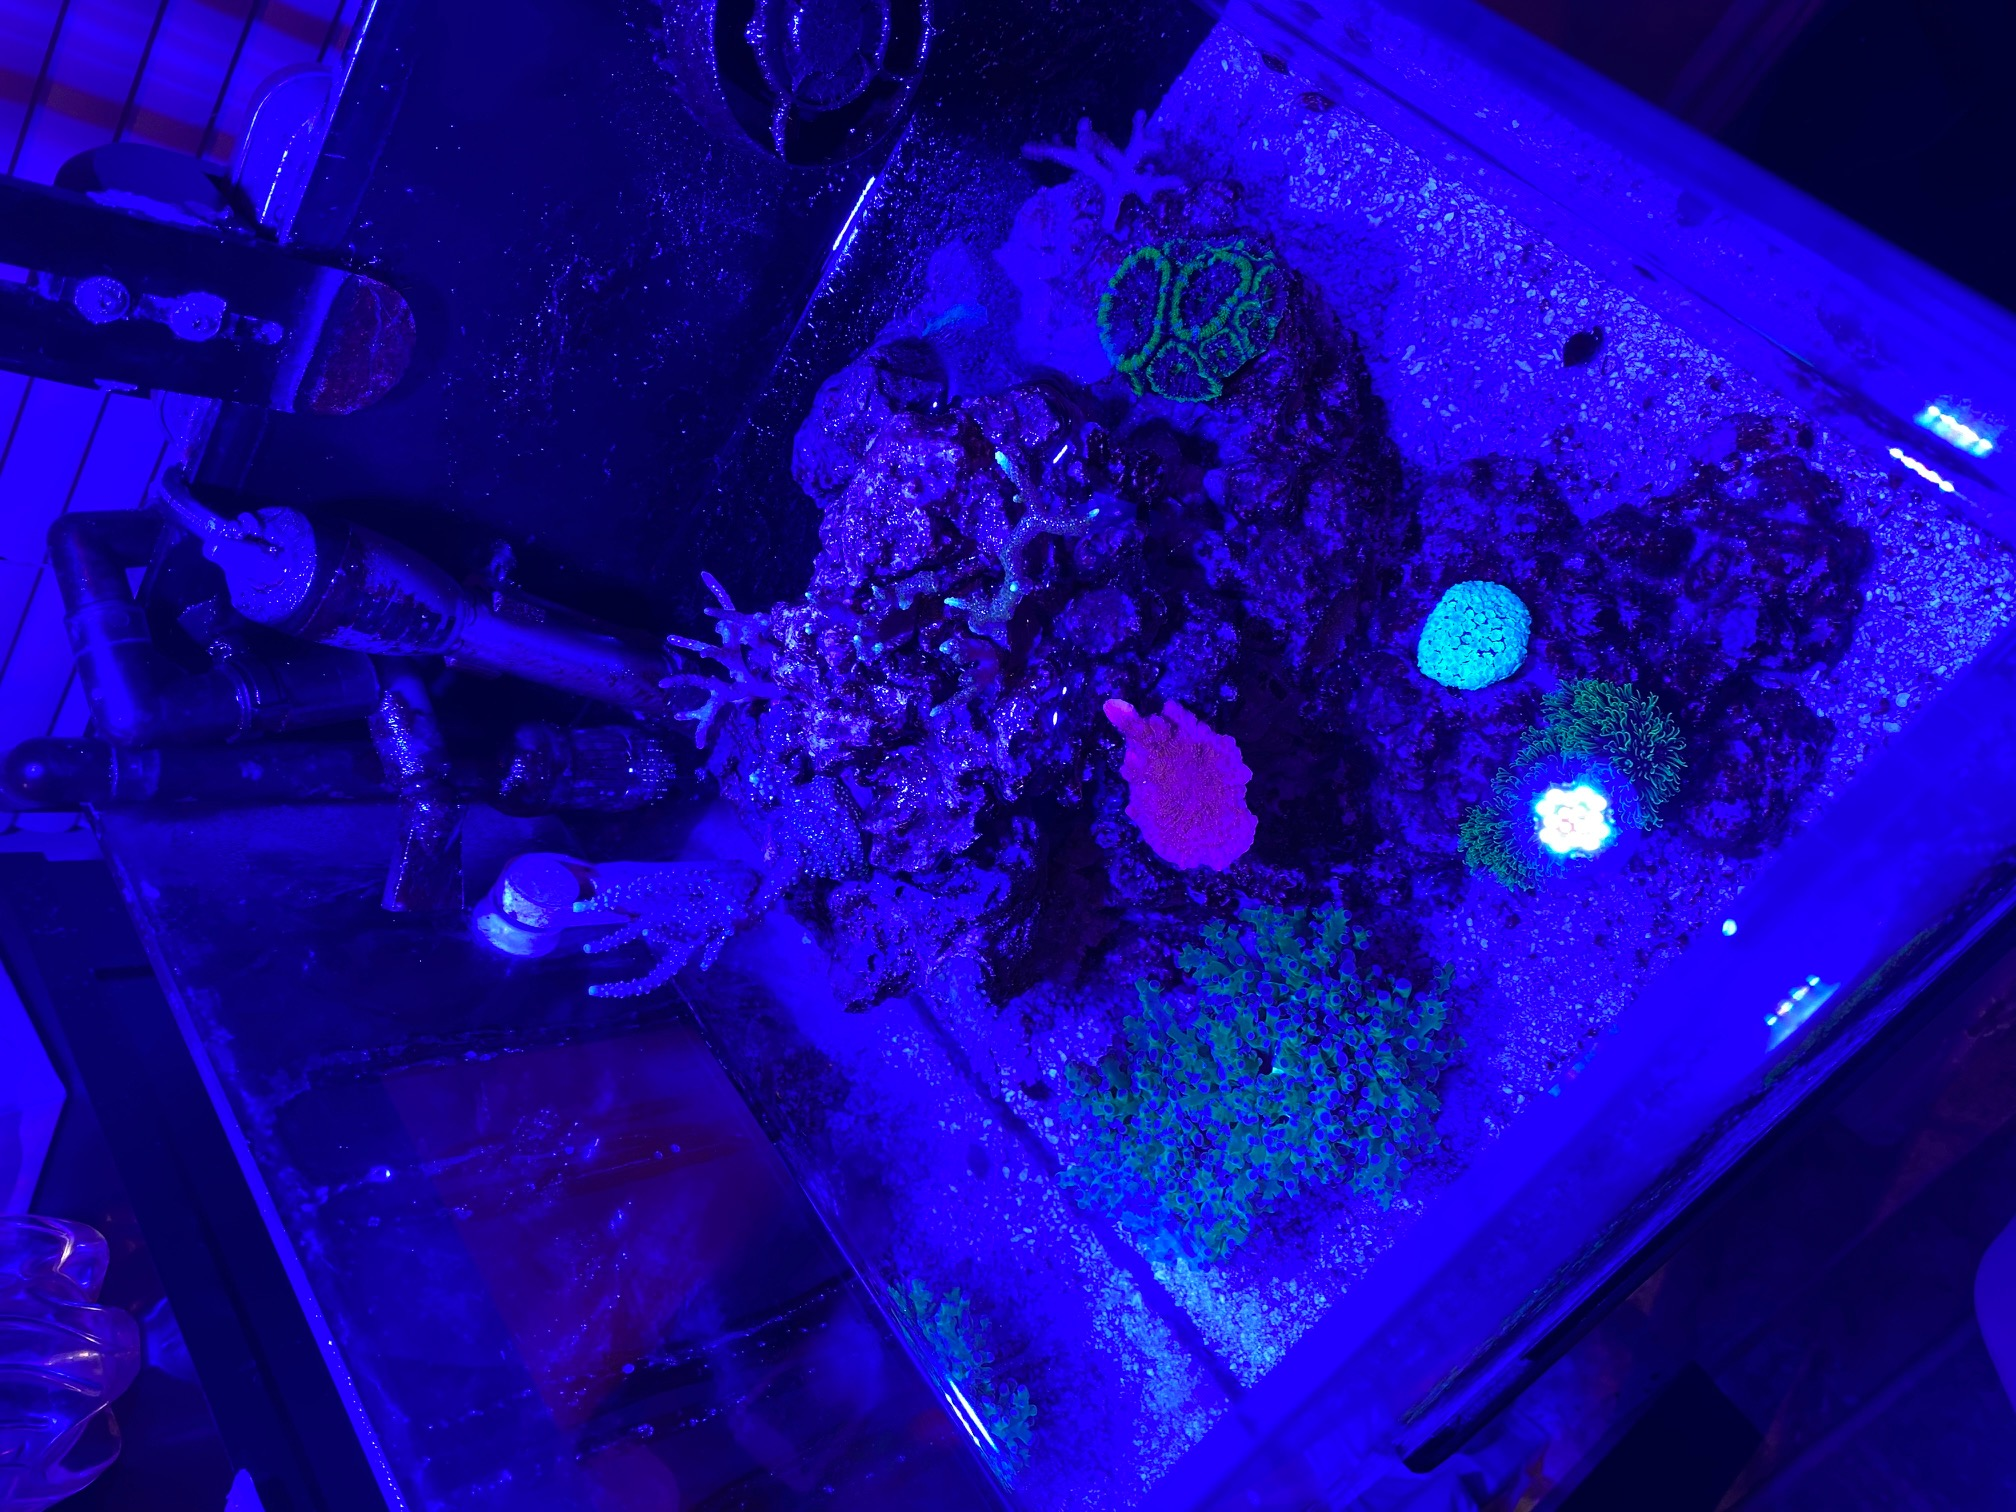
\includegraphics[width=0.74125\textwidth, angle=-90]{EmptyAquarium.jpg}
    \caption{Reef tank mid water change}
\end{figure}


\end{document}
